% ****************************************************************************************** % Dissertation template and document class for Princeton University
% Author  : Jeffrey Scott Dwoskin <jdwoskin@princeton.edu>
% Adapted from: http://www.math.princeton.edu/graduate/tex/puthesis.html
% ****************************************************************************************** %


%%% For print copies
%% set 'singlespace' option to set entire thesis to single space, and define "\printmode" to remove all hyperlinks for printed copies of the thesis. Delete all output files before changing this mode -- it will turn hyperref package on and off
%\documentclass[12pt,lot, lof, singlespace]{puthesis}
%\newcommand{\printmode}{}

%%% For the electronic copy, use doublespacing, define "\proquestmode" to use outlined links, instead of colored links. 
\documentclass[12pt,lot, lof]{puthesis}
\newcommand{\proquestmode}{}
% I prefer proquestmode to be off for electronic copies for normal use, since the colored links are less distracting. However when printed in black and white, the colored links are difficult to read. 

%%% For early drafts without some of the frontmatter
% Also see the "ifodd" command below to disable more frontmatter
%\documentclass[12pt]{puthesis}

%%%%%%%%%%%%%%%%%%%%%%%%%%%%%%%%%%%%%%%%%%%%%%%%%%%%%%%%%%%%%\
%%%% Author & title page info

\title{\textbf{
% Gauge Theory and the
Magnetic Monopoles, `t Hooft Lines,
\\ {\Large and the}
\\ Geometric Langlands Correspondence}}

\submitted{Spring 2018}  % degree conferral date (January, April, June, September, or November)
\copyrightyear{2018}  % year in which the copyright is secured by publication of the dissertation.
\author{Alexander B. Atanasov}
\advisor{Philsang Yoo}  %replace with the full name of your advisor
% \departmentprefix{Program in}  % defaults to "Department of", but programs need to change this.
\department{Mathematics}

%%%%%%%%%%%%%%%%%%%%%%%%%%%%%%%%%%%%%%%%%%%%%%%%%%%%%%%%%%%%%\
%%%% Tweak float placements
% From: http://mintaka.sdsu.edu/GF/bibliog/latex/floats.html "Controlling LaTeX Floats"
% and based on: http://www.tex.ac.uk/cgi-bin/texfaq2html?label=floats
% LaTeX defaults listed at: http://people.cs.uu.nl/piet/floats/node1.html

% Alter some LaTeX defaults for better treatment of figures:
    % See p.105 of "TeX Unbound" for suggested values.
    % See pp. 199-200 of Lamport's "LaTeX" book for details.
    %   General parameters, for ALL pages:
    \renewcommand{\topfraction}{0.85}	% max fraction of floats at top
    \renewcommand{\bottomfraction}{0.6}	% max fraction of floats at bottom
    %   Parameters for TEXT pages (not float pages):
    \setcounter{topnumber}{2}
    \setcounter{bottomnumber}{2}
    \setcounter{totalnumber}{4}     % 2 may work better
    \setcounter{dbltopnumber}{2}    % for 2-column pages
    \renewcommand{\dbltopfraction}{0.66}	% fit big float above 2-col. text
    \renewcommand{\textfraction}{0.15}	% allow minimal text w. figs
    %   Parameters for FLOAT pages (not text pages):
    \renewcommand{\floatpagefraction}{0.66}	% require fuller float pages
	% N.B.: floatpagefraction MUST be less than topfraction !!
    \renewcommand{\dblfloatpagefraction}{0.66}	% require fuller float pages

% The documentclass already sets parameters to make a high penalty for widows and orphans. 

%%%%%%%%%%%%%%%%%%%%%%%%%%%%%%%%%%%%%%%%%%%%%%%%%%%%%%%%%%%%%\
%%%% Use packages

\usepackage{amsmath,amssymb,amsfonts,amsthm}
\usepackage{gensymb}
\usepackage{tikz-cd}
\usepackage{mathtools}
%%% For figures
\usepackage{graphicx}
%%% For tables
\usepackage{tabularx}
\newcolumntype{Y}{>{\centering\arraybackslash}X}
%\usepackage{subfig,rotate}

%%% for comments
\usepackage{verbatim}

%%% For tables
\usepackage{multirow}
% Longtable lets you have tables that span multiple pages.
\usepackage{longtable}

% Booktabs produces far nicer tables than the standard LaTeX tables.
%   see: http://en.wikibooks.org/wiki/LaTeX/Tables
\usepackage{booktabs}

%set parameters for longtable:
% default caption width is 4in for longtable, but wider for normal tables
\setlength{\LTcapwidth}{\textwidth}



%%%%%%%%%%%%%%%%%%%%%%%%%%%%%%%%%%%%%%%%%%%%%%%%%%%%%%%%%%
%%% Printed vs. online formatting
\ifdefined\printmode

% Printed copy
% url package understands urls (with proper line-breaks) without hyperlinking them
\usepackage{url}


\else

\ifdefined\proquestmode
%ProQuest copy -- http://www.princeton.edu/~mudd/thesis/Submissionguide.pdf

% ProQuest requires a double spaced version (set previously). They will take an electronic copy, so we want links in the pdf, but also copies may be printed or made into microfilm in black and white, so we want outlined links instead of colored links.
\usepackage{hyperref}
\hypersetup{bookmarksnumbered}

% copy the already-set title and author to use in the pdf properties
\makeatletter
\hypersetup{pdftitle=\@title,pdfauthor=\@author}
\makeatother

\else
% Online copy

% adds internal linked references, pdf bookmarks, etc

% turn all references and citations into hyperlinks:
%  -- not for printed copies
% -- automatically includes url package
% options:
%   colorlinks makes links by coloring the text instead of putting a rectangle around the text.
\usepackage{hyperref}
\hypersetup{colorlinks,bookmarksnumbered}

% copy the already-set title and author to use in the pdf properties
\makeatletter
\hypersetup{pdftitle=\@title,pdfauthor=\@author}
\makeatother

% make the page number rather than the text be the link for ToC entries
%\hypersetup{linktocpage}
\fi % proquest or online formatting
\fi % printed or online formatting


%%%%%%%%%%%%%%%%%%%%%%%%%%%%%%%%%%%%%%%%%%%%%%%%%%%%%%%%%%%%%\
%%%% Define commands

% Define any custom commands that you want to use.
% For example, highlight notes for future edits to the thesis
%\newcommand{\todo}[1]{\textbf{\emph{TODO:}#1}}


% create an environment that will indent text
% see: http://latex.computersci.org/Reference/ListEnvironments
% 	\raggedright makes them left aligned instead of justified
\newenvironment{indenttext}{
    \begin{list}{}{ \itemsep 0in \itemindent 0in
    \labelsep 0in \labelwidth 0in
    \listparindent 0in
    \topsep 0in \partopsep 0in \parskip 0in \parsep 0in
    \leftmargin 1em \rightmargin 0in
    \raggedright
    }
    \item
  }
  {\end{list}}

% another environment that's an indented list, with no spaces between items -- if we want multiple items/lines. Useful in tables. Use \item inside the environment.
% 	\raggedright makes them left aligned instead of justified
\newenvironment{indentlist}{
    \begin{list}{}{ \itemsep 0in \itemindent 0in
    \labelsep 0in \labelwidth 0in
    \listparindent 0in
    \topsep 0in \partopsep 0in \parskip 0in \parsep 0in
    \leftmargin 1em \rightmargin 0in
    \raggedright
    }

  }
  {\end{list}}



%%%%%%%%%%%%%%%%%%%%%%%%%%%%%%%%%%%%%%%%%%%%%%%%%%%%%%%%%%%%%\
%%%% Front-matter

% For early drafts, you may want to disable some of the frontmatter. Simply change this to "\ifodd 1" to do so.
\ifodd 0
% front-matter disabled while writing chapters
\renewcommand{\maketitlepage}{}
\renewcommand*{\makecopyrightpage}{}
\renewcommand*{\makeabstract}{}

% you can just skip the \acknowledgements and \dedication commands to leave out these sections.

\else


\abstract{
% Abstract can be any length, but should be max 350 words for a Dissertation for ProQuest's print indicies (150 words for a Master's Thesis) or it will be truncated for those uses.
The aim of this thesis is to give the reader a gentle but thorough introduction to the vast web of ideas underlying the realization of the geometric Langlands correspondence in the physics of quantum field theory (QFT). It begins with a pedagogically-motivated introduction to the relevant concepts in the Langlands program, quantum field theory, and gauge theory for an audience of mathematicians or physicists. With this machinery in place, the more complicated phenomena associated with gauge theory is explored, specifically instantons, topological operators, and electric-magnetic duality. We conclude by connecting the ideas of the Langlands correspondence discussed at the start with phenomena in topologically twisted $\mathcal N = 4$ supersymmetric Yang-Mills theory (SYM) which exhibits a striking property known as $S$-duality. A large part of the goal of this thesis is to give an exposition to the language and techniques that the literature related to this topic already assumes familiarity with, so that an advanced undergraduate or early graduate student might have a good exposition into this field. 
}

% \acknowledgements{
% %I would like to thank...
% I would like to firstly thank Professor Yoo for agreeing to be my advisor and for dedicating much of his time (not to mention his Monday lunches) to help guide me along as I worked through understanding the many ideas necessary to write this thesis. I especially want to thank him for his patience when I was struggling with the more difficult parts of this program, and for his excellent ability to get to the heart of matters in pointing out what was important for me to understand.

I would also like to thank the past professors that I have had at Yale for building my background up so that I could complete this thesis. In particular, I would like to thank Prof. David Poland for giving me the unique opportunity to get my hands dirty working with conformal theory early in my undergraduate career, and for his guidance throughout my time at Yale. Second, I would like to thank Professors Igor Frenkel and Walter Goldberger for providing me the courses that challenged me and pushed me to the furthest limits of any other academic experience at Yale.

Lastly, I would like to thank my friends and colleagues, Aaron Hillman and Andrew Saydjari, for being part of this great journey with me. I want to thank them for the numerous and deeply meaningful conversations that they engaged me with. I wish them all the best in their future scientific pursuits, and look forward to seeing them fly.
% }

% \dedication{To my parents.}

\fi  % disable frontmatter


%%%%%%%%%%%%%%%%%%%%%%%%%%%%%%%%%%%%%%%%%%%%%%%%%%%%%%%%%%%%%\
%%%% Hide some chapters

%%% If you want to produce a pdf that includes only certain chapters, specify them with includeonly, in addition to including all chapters below.
%\includeonly{ch-intro/chapter-intro}
%%% You can also specify multiple chapters.
%\includeonly{ch-intro/chapter-intro,ch-usage/chapter-usage}
%\includeonly{chap1,chap2,chap3}


\newtheorem{theorem}{Theorem}[section]
\newtheorem{lemma}[theorem]{Lemma}
\newtheorem{prop}[theorem]{Proposition}
\newtheorem{conj}[theorem]{Conjecture}
\newtheorem{cor}[theorem]{Corollary}
\newtheorem{obs}[theorem]{Observation}
\newtheorem{ind}[theorem]{Indication}
\newtheorem{mot}[theorem]{Motivation}
\newtheorem{fact}[theorem]{Fact}
\newtheorem{goal}{Goal}
\newtheorem{idea}[theorem]{Idea}

\theoremstyle{remark}
\newtheorem*{review}{Review}
\newtheorem*{ques}{Question}
\newtheorem*{nb}{Note}

\theoremstyle{definition}
\newtheorem{defn}[theorem]{Definition}
\newtheorem{phys}[theorem]{Physical Concept}
\newtheorem{concept}[theorem]{Concept}
\newtheorem{view}{View}
\newtheorem{cons}[theorem]{Construction}
\newtheorem{eg}[theorem]{Example}

\def\lacts{\,\ensuremath{%
  \reflectbox{\rotatebox[origin=c]{180}{$\circlearrowleft$}}}\,}
\def\racts{\,\ensuremath{%
    \reflectbox{\rotatebox[origin=c]{180}{$\circlearrowright$}}}\,}
\def\spec{\mathrm{Spec}\,}
\def\maxspec{\mathrm{MaxSpec}\,}
\def\dd{\mathrm{d}}
\def\im{\mathrm{im}\,}
\def\zz{\mathbb{Z}}
\def\rr{\mathbb{R}}
\def\cc{\mathbb{C}}
\def\cp{\mathbb{CP}}
\def\qq{\mathbb{Q}}
\def\ff{\mathbb{F}}
\def\kk{\mathbf{k}}
\def\fq{\mathbb{F}_q}
\def\fp{\mathbb{F}_p}
\def\gg{\frak{g}}
\def\gl{\frak{gl}}
\def\sl{\frak{sl}}
\def\su{\frak{su}}
\def\so{\frak{so}}
\def\SU{\mathrm{SU}}
\def\SO{\mathrm{SO}}
\def\GL{\mathrm{GL}}
\def\SL{\mathrm{SL}}
\def\Gal{\mathrm{Gal}}
\def\tr{\mathrm{Tr}\,}
\def\Ad{\mathrm{Ad}\,}
\def\ad{\mathrm{ad}\,}
\def\OO{\mathcal{O}}

\makeatletter
\def\@tempa#1{\@xp\@tempb\meaning#1\@nil#1}
\def\@tempb#1>#2#3 #4\@nil#5{%
  \@xp\ifx\csname#3\endcsname\mathaccent
    \@tempc#4?"7777\@nil#5%
  \else
    \PackageWarningNoLine{amsmath}{%
      Unable to redefine math accent \string#5}%
  \fi
}
\def\@tempc#1"#2#3#4#5#6\@nil#7{%
  \chardef\@tempd="#3\relax\set@mathaccent\@tempd{#7}{#2}{#4#5}}
\@tempa\widehat
\makeatother

%%%%%%%%%%%%%%%%%%%%%%%%%%%%%%%%%%%%%%%%%%%%%%%%%%%%%%%%%%%%%
%%%% Notes:

% Footnotes should be placed after punctuation.\footnote{place here.}
% Generally, place citations before the period~\cite{anotherauthor}.
% The proper usage for i.e., and e.g., include commas ``(e.g., option A, option B)''

%%%%%%%%%%%%%%%%%%%%%%%%%%%%%%%%%%%%%%%%%%%%%%%%%%%%%%%%%%%%%
%%%% Import chapters

\begin{document}

\makefrontmatter


% If you've disabled frontmatter, you can insert the toc manually
% \maketitle
% \tableofcontents%\clearpage

% \include lets us split up the document (and each include starts a new page):
\chapter{Introduction and Overview of the Langlands Program\label{ch:intro}}

The aim of this chapter is to give a gentle conceptual and historical overview of both the Langlands program and the development of quantum and conformal field theories. The goal is not so much to develop any mathematical background so much as to illustrate to the reader \emph{why} this great web of ideas is important.

The following two sections are adopted from the lectures and notes of \cite{Yoo18}. The third and fourth are motivations adopted from the first lecture of \cite{Yoo17} together with various ideas of \cite{Yoo18}.

\section{The Langlands Program in Number Theory} % (fold)
\label{sec:the_langlands_program_in_number_theory}

\emph{Fermat's Last Theorem}, once known as the ``greatest unsolved problem in mathematics,'' asserts that there does not exist an integral solution to
\begin{equation}
\label{eqn:fermat-last-theorem}
a^n + b^n = c^n, \qquad n > 2
\end{equation}
with $abc\neq 0$. 

The proof of Fermat's last theorem relied on some of the most intricate mathematics developed at the end of the 20th century. A crucial step towards its completion was put forward by Frey and made rigorous by Ribet and Serre. They showed that if the triple $(a,b,c)$ was a solution to (\ref{eqn:fermat-last-theorem}) for and odd prime $n=p$ (which one might assume without loss of generality), then the so-called Frey curve $y^2=x(x-a^p)(x+b^p)$ contradicted Taniyama-Shimura-Weil conjecture, now referred to as the Modularity Theorem. 
\begin{theorem}[Modularity Theorem for Elliptic Curves]
\label{thm:modularity-theorem}
	Every elliptic curve is modular.
\end{theorem}

Fermat's last theorem follows from a special case of the modularity conjecture. The modularity conjecture for elliptic curves turns out to follow from a special case of a special case of the \emph{Langlands conjectures}, originally formulated by Robert Langlands in a letter to Andre Weil in 1967 \cite{langlands1967}.
More precisely, it is a corollary of the Langlands correspondence for $G = \mathrm{GL}_2$ over $\qq$ \footnote{In fact, the modularity theorem is strictly stronger than necessary. It was enough for Wiles and Taylor to prove that a special family (the so-called semistable ones) of elliptic curves is modular. The case for general elliptic curves has since been proven by Breuil, Conrad, Diamond, and Taylor \cite{breuil2001}.}. This part of the Langlands conjecture remains unproven as of May 2018. 

We give a sketch of the statement of the number-theoretic Langlands correspondence, intended towards an audience with some background in \emph{Galois theory} and the language of \emph{adeles}. 

Begin by considering the \textbf{absolute Galois group} of the rationals:
\[
	\mathrm{Gal}(\overline{\qq}/\qq),
\]
where $\overline{\qq}$ is the algebraic closure of $\qq$, consisting of all algebraic numbers. This Galois group is tremendously large. It is the profinite group obtained as an inverse limit over all finite Galois extensions of $\qq$. It is an open conjecture whether every finite group appears as a Galois group of some Galois extension. 
\begin{conj}[Inverse Galois]
	Every finite group is contained in $\mathrm{Gal}(\overline{\qq}/\qq)$.
\end{conj}
The number theoretic Langlands correspondence considers the $n$-dimensional representations of the absolute Galois group (called \emph{Galois representations}) and relates them to certain representations known as \emph{automorphic representations}. To define these latter types of representations, we first make the definition
\begin{defn}[Ring of adeles]
	The \textbf{ring of adeles} of $\qq$ is defined as 
	\[
		\mathbb A_{\qq} := \rr \times \prod_{p\, \mathrm{prime}}^{res} \qq_p,
	\]
	where $\qq_p$ denotes the $p$-adic completion of the rationals \cite{bachman1964} ($\rr$ can be viewed as the completion at $p=\infty$) and the above product is \emph{restricted} in the sense that:
	\[
		\prod_{p\, \mathrm{prime}}^{res} \qq_p := \left\{ (x_p) \in \prod_{p\, \mathrm{prime}} \qq_p \mid x_p \in \mathbb Z_p \text{ for all but finitely many } p\right\}.
	\]
\end{defn}
Let $\GL_n(\mathbb A_\qq)$ denote the set of $n \times n$ matrices with entries in $\mathbb A_\qq$. Further, because $\qq \hookrightarrow \mathbb A_\qq$ diagonally, we also have 
\[
	\GL_n(\qq) \hookrightarrow \GL_n(\mathbb A_\qq)
\]
which yields a left (and right) action\footnote{In this paper we shall use $G\lacts X$ to denote left action of $G$ on $X$ and $X \racts G$ to denote right action.}:
\[
	\GL_n(\qq) \lacts  \GL_n(\mathbb A_\qq) \racts  \GL_n(\qq).
\]
The left quotient space $\GL_n(\qq) \backslash \GL_n(\mathbb A_\qq)$ is well-defined in this case. Since $\GL_n(\qq)$ still acts by right action on this space, functions of this space form a (left) representation of $\GL_n(\qq)$
\[
	\GL_n(\qq) \lacts \mathrm{Fun}\left( \GL_n(\qq) \backslash \GL_n(\mathbb A_\qq) \right)
\]
This can be decomposed into irreducible representations, which are known as the \textbf{automorphic representations} of $\GL_n(\qq)$.
Though not absolutely precise, this is a good first-order description of what an automorphic representation is. 

\begin{idea}
	The Langlands correspondence associates to each $n$-dimensional representation of the absolute Galois group $\mathrm{Gal}(\bar \qq/\qq)$ an automorphic representation of $\GL_n(\qq)$.
\end{idea}
More than just an equivalence of sets, though, the Langlands correspondence states that a certain set of \emph{eigenvalue data} must agree on both sides. 

From the perspective of the absolute Galois group (henceforth referred to as the \emph{Galois side}), this eigenvalue data is called the \textbf{Frobenius eigenvalues} of this representation. For $p$ an unramified prime, the Frobenius automorphism $x \to x^p$ is the generator of the Galois group of any finite extension $\mathrm{Gal}(\mathbb F_q/\mathbb F_p)$. Given a finite-dimensional representation of $\mathrm{Gal}(\bar \qq/\qq)$ as well as a conjugacy class, one can lift the Frobenius automorphism to a conjugacy class. The eigenvalues (well-defined for a given conjugacy class) of these elements are the Frobenius eigenvalues of that representation. 

From the perspective of the automorphic representations (henceforth referred to as the \emph{automorphic side}), the eigenvalue data is more difficult to describe. It relies on the construction of linear operators on the space of automorphic representations known as \textbf{Hecke Operators}. Though a full description of the Hecke eigendata is beyond the scope of this paper, we can give a rough and ``cartoonish'' picture of the most basic case of Hecke eigenvalues (c.f. \cite{miyake1971, kudla2004} for a deeper exposition). In the $\GL_2$ case, the space of automorphic representations is related to the space of modular forms on the upper half plane corresponding to quotients $\Gamma \backslash \mathbb H$ with $\Gamma$ a special type of discrete subgroup of $\SL_2(\mathbb Z)$. 

When $\Gamma = \SL_2(\mathbb Z)$, a modular form of weight $k$ can be interpretted as a function $f$ on the set of lattices in $\mathbb R^2$ so that $f(a\Lambda) = a^k f(\Lambda)$.
The $m$th Hecke operator is then defined as:
\[
	T_m f (\Lambda) := m^{k-1} \sum_{[\Lambda' : \Lambda] = m} f(\Lambda')
\]
These are pairwise-commuting linear operators, and can thus be simultaneously diagonalizable. 
The modular forms that are eigenvectors for this operator are known as \textbf{Hecke eigenforms}, and their eigenvalue data is what we define as the \textbf{Hecke eigenvalues} of that representation. The story for more general subgroups $\Gamma$ gives an analogous construction but the story becomes much more involved beyond the $\GL_2$ case.


With this bare background laid out, we can make at least a parsable statement of the Langlands conjecture.

\begin{conj}[Langlands]
	To each $n$-dimensional representation of the absolute Galois group, there is a corresponding automorphic representation of $\GL_n(\qq)$ so that the Frobenius eigenvalues of the Galois representation agree with the Hecke eigenvalues of the automorphic representation.
\end{conj}

It is worth mentioning that the Langlands conjecture over $G = \mathrm{GL}_1$ is the same as what is known in number theory as \emph{class field theory} \cite{frenkel2007}. 


Many questions in number theory can be formulated in terms of questions about the nature of the absolute Galois group. On the other hand, automorphic representations can be studied using analytic methods, which would imply that deep number-theoretic data can be made accessible by studying these analytic objects.

The eigenvalue data plays a particularly important role both in the Langlands correspondence and its geometric analogue. The study of this eigenvalue data will become the study of the \emph{geometric Satake} symmetries acting on both sides of the geometric Langlands equivalence, and this thesis will explore how ideas from physics can give a concrete realization of the eigenvalue data in terms of \emph{operator insertions} in quantum field theory \cite{kapustin2006}. 

% section the_langlands_program (end)

\section{Weil's Rosetta Stone and Geometric Langlands} % (fold)
\label{sec:weil_s_rosetta_stone_and_geometric_langlands}

The Langlands correspondence in number theory also has a close analogy for curves defined over finite fields $\mathbb F_q$. Indeed, translating the number theoretic statements of the Langlands program has over the past fifty years led to an extremely fruitful set of developments in the field of \emph{Arithmetic Geometry}. These developments have led to the famous proofs of the \emph{Weil Conjectures} and the \emph{Riemann Hypothesis over Finite Fields}. We will not discuss these developments here but refer the reader to \cite{osserman2008}. 

We \emph{will}, however, illustrate this anology to function fields over $\mathbb F_q$ to motivate the translation of the Langlands program to a more geometric setting. Consider the 1-dimensional affine space $\mathbb A^1 (\mathbb F_q)$. We have $F := \mathbb F_q(t)$ the function field on $\mathbb A^1 (\mathbb F_q)$. This will play the role analogous to the role of $\qq$ before. Before, we could complete $\qq$ at each prime $p$ to get the $p$-adics. For each point $x \in \mathbb A^1 (\mathbb F_q)$, there is a notion of a \emph{completion} for $\mathbb F_q(t)$ at $x$, and also a notion of a \emph{ring of integers} corresponding to the localization $\mathcal O_x$ at $x$.

To understand these completions, we make the following definitions.
\begin{defn}[Formal Power Series]
	Let $\kk[t]$ be a polynomial ring in one variable over a field $\kk$. The \textbf{ring of formal power series} around $x$, $\kk[[t-x]]$, is defined as the ring of all (possibly infinite) series of the form
	\[
		\sum_{n=0}^\infty a_n q^n,
	\]
	where here there is no restriction that only finitely many $a_n$ are nonzero. 
\end{defn}

\begin{defn}[Formal Laurent Series]
	Let $\kk[t]$ be a polynomial ring in one variable over a field $\kk$. The \textbf{ring of formal Laurent series} around $x$, $\kk((t-x))$, is defined as the ring of all (possibly infinite) series of the form
	\[
		\sum_{n=-\infty}^\infty a_n q^n,
	\]
	where here there is no restriction that only finitely many $a_n, n \geq 0$ are nonzero but \emph{only finitely many $a_n, n<0$ can be nonzero}.
\end{defn}

The field $F_x$ corresponding to the completion of $F$ at $x$ can be viewed as the field of Laurent series around $x$, denoted $\mathbb F_q((t-x))$. $\mathcal O_x$ can similarly be viewed in terms of formal power series at $x$, $\mathbb F_q [[t-x]]$. With this machinery in place, we can define the ring of adeles analogously to before.

\begin{defn}[Adele Ring for $\mathbb F_q(t)$]
	The ring of adeles of $\mathbb F_q(t)$ is defined as 
	\[
		\mathbb A_{\mathbb F_q(t)} := \prod_{x \in \mathbb P^1(\mathbb F_q)}^{res} \mathbb F_{q_x}((t-x))
	\]
	and the above product is restricted as before in the sense that all but finitely many terms in this product over $x$ lie in $\mathbb F_q [[t-x]]$. Here the completion at the point at infinity corresponds to $\mathbb F_q ((1/t))$.
\end{defn}
We naturally have that 
\[
	\mathbb O_{\mathbb F_q(t)} := 	\prod_{x \in \mathbb P^1(\mathbb F_q)} \mathbb F_{q_x}[[t-x]]
\]
sits inside $\mathbb A_{\mathbb F_q(z)}$.

All of this can be translated more generally to the function field $F$ for a curve $C$ over $\mathbb F_p$. This would correspond to a number field and its ring of integers in the original Langlands conjecture. Here, ramification of various points on the curve becomes an issue and there is more subtlety in defining many of the above concepts.

Already, for a function field of a curve $C$, the analogue of the Galois group is known to be the \textbf{etale fundamental group}, and a Galois representation would be a representation of $\pi_1^{\text{\'et}}(C,x) \to \GL_n$ in the unramified case. In analytic language for $C$ a complex curve, the \'etale fundamental group becomes the usual $\pi_1$ and a Galois representation becomes a representation of the fundamental group $\pi_1(C) \to \GL_n$. 

In the unramified case, automorphic representations correspond exactly the the $\GL_n(\mathbb O_F)$-invariant functions on $\GL_n (\mathbb F)\backslash \GL_n(\mathbb A_F)$. This means that the space of automorphic representations corresponds to:
\[
	\mathrm{Fun} \left(\GL_n (\mathbb F)\backslash \GL_n(\mathbb A_F)/\GL_n(\mathbb O_F) \right).
\]

It is the following theorem of Weil that will be crucial in making a connection between with the geometric setting over $\cc$.
\begin{theorem}[Weil Uniformization]
	Take $F$ the function field for a curve $C$ over $\fq$. There is a canonical bijection as sets between
	\[
		G (\mathbb F)\backslash G(\mathbb A_F)/G(\mathbb O_F)
	\]
	and the set of $G$-bundles over $C$. Moreover, this in fact extends to an algebraic correspondence between this space and the stack $\mathrm{Bun}_G(C, \fq)$. 
\end{theorem}

$G$-bundles are discussed in Section~\ref{sub:principal_bundles}.
So (in the unramified case), the automorphic side is captured by functions on $\mathrm{Bun}_G(C, \fq)$. 
This set of functions admits an action by the \textbf{spherical Hecke algebra} at every closed point $x \in C$, defined as the space of compactly supported functions on the double coset space:
\[
	\mathcal H_x := \mathrm{Fun}_c (\GL_n (\mathcal O_x)\backslash \GL_n(F_x)/\GL_n(\mathcal O_x))
\]
with multiplication given by an operation known as a \textbf{convolution product} of functions. These algebras correspond to the Hecke operators described earlier. The actions of these algebras at different $x$ commute with one another, just like the Hecke operators in the first column. Consequently, they can be simultaneously diagonalized to give rise to eigenfunctions generalizing the notion of Hecke eigenforms in the number-theoretic $\GL_2$ setting. More correctly, these operators yield eigen-objects called \textbf{Hecke-eigensheaves}\footnote{For an explanation about the transition between functions on this coset space and sheaves, see a reference on the \emph{function-sheaf correspondence}, e.g. \cite{shin2005}}. This thesis will aim to explore the corresponding interpretation of this action in the context of topological field theory in physics.

\begin{table}[t]
	\centering
	\setlength\tabcolsep{3pt} 
\begin{tabularx}{\linewidth}{|>{\hsize=0.8\hsize}Y|>{\hsize=1.2\hsize}Y|Y|}
	\hline
	Number Theory & Curves over $\ff_q$ & Riemann Surfaces\\
	\hline
	\hline
	$\zz \subset \qq$ & $\ff_q[t] \subset \ff_q(t)$ & $\OO^{hol}_\cc \subset \OO^{mer}_\cc$ \\
	\hline
	$\spec \zz$ & $\mathbb A^1_{\ff_q}$ & $\cc$\\
	\hline
	$\spec \zz \cup \{\infty\}$ & $\mathbb P^1_{\ff_q}$ (projective line) & $\cp^1$ (Riemann sphere)\\
	\hline
	$p$ prime number & $x \in \mathbb A^1_{\ff_q}$ & $x \in \cc$\\
	\hline
	\hline
	$\zz_p$ ($p$-adic integers) & $\ff_q[[t-x]]$ power series around $x$ & $\cc[[z-x]]$ holomorphic on formal disk around $x$\\
	\hline
	$\qq_p$ ($p$-adic numbers) & $\ff_q((t-x))$ Laurent series around $x$ & $\cc((z-x))$ holomorphic on punctured formal disk around $x$\\
	\hline
	$\mathbb A_\qq$ (adeles) & $\mathbb A_{\ff_q}$ function field adeles & $\prod_{x \in \cc}^{res} \cc((z-x))$ restricted product of functions on all punctured disks, with all but finitely many extending to the unpunctured disk\\
	\hline
	\hline
	$F/\qq$ (number fields) & $F/\ff_q(t)$ or $\ff_q(C)/\ff_q(\mathbb P^1)$ & $C \to \cp^1$ (branched covers)\\
	\hline
	$\mathrm{Gal}(\overline{F}/F)$ & $\mathrm{Gal}(\overline{F}/F) = \pi_1^{\text{\'et}}(\spec F, \spec \bar F)$ & \\
	\hline
	& $\twoheadrightarrow \mathrm{Gal}(F^{\text{unr}}/F) = \pi_1^{\text{\'et}}(C, x)$ & $\pi_1(C, x)$\\ 
	\hline
	\hline
\end{tabularx}
\caption{Weil's \emph{Rosetta stone}}
\label{tab:rosetta}
\end{table}

Table~\ref{tab:rosetta}, based off of \cite{Yoo18} and \cite{nlab:function_field_analogy}, captures the analogy described above. This is the \emph{function field analogy}, otherwise known as Weil's \emph{Rosetta stone}. 

It is the hope and goal of this correspondence that the extremely difficult number-theoretic Langlands program might become more accessible when phrased in the language of the second or third columns of Table~\ref{tab:rosetta}. A reason to believe this might be so is because the power of modern algebraic geometry, as developed by Grothendieck, Serre, Deligne, and others, becomes a prominent force in driving our understanding of columns two and three. 

The analogy between columns one and two is especially strong, and in many cases a statement about the second column can be exactly translated over into a statement about the first. % The Langlands program for the second column would relate an $n$-dimensional representation of $\Gal(\overline F/F)$ to some special ``automorphic'' subrepresentation of $\mathrm{Fun}(\GL_n (\mathbb F)\backslash \GL_n(\mathbb A_F))$ with some associated eigenvalue data on both sides corresponding appropriately.


We are now in a place where we can attempt to discuss and motivate the third column: the geometric Langlands correspondence over $\cc$. To do this, we will begin with motivation from a different direction, namely Fourier analysis.


% section weil_s_rosetta_stone_and_geometric_langlands (end)

\section{The Fourier Transform and Pontryagin Duality} % (fold)
\label{sec:the_fourier_transform_and_pontryagin_duality}
		
In this section, we will attempt to give an alternative motivation for the geometric Langlands program as a generalized non-abelian analogue of the Fourier transform. 

First let us begin by working with a locally-compact abelian group $G$. Recall that these possess a unique (normalized) Haar measure. We make the following definition:
\begin{defn}[Unitary Character]
	For $G$ locally-compact and abelian, a \textbf{unitary character} of $G$ is a group homomorphism $\chi: G \to U(1)$.
\end{defn}
Using this definition, we define the following group, which plays a role as a \emph{dual} to $G$. It is called the \textbf{Pontryagin dual}.
\begin{defn}
	The set of all unitary characters $\chi$ together with multiplication  $\chi_1 \cdot \chi_2 \in \mathrm{Hom}(G, U(1))$ given by pointwise multiplication of characters, form an abelian group, denoted by $\widehat{G}.$
\end{defn}

\begin{eg}
	We have the following examples:
	\begin{enumerate}
		\item Let $G = S^1$, then the space of unitary characters consists precisely of these of the form $e^{inx}: G \to U(1)$. This makes $\widehat G = \mathbb Z$.
		\item Let $G = \mathbb Z$, then $\chi(1)$ determines the representation uniquely, and so $\widehat G = U(1)$.
		\item 			Let $G = \mathbb R$, then $e^{ikx} : \mathbb R \to U(1)$ is free to have $k$ vary over $\mathbb R$ so $\widehat G = \mathbb R$.
	\end{enumerate}

\end{eg}

Notice in all these cases that $\widehat{\widehat G} \cong G$. This is in fact true more general, and we have the following theorem:
\begin{theorem}[Pontryagin Duality]
For any locally-compact abelian topological group $G$, the canonical map 
\begin{equation*}
\begin{split}
G &\to \widehat{\widehat G}\\
g &\mapsto [\chi \mapsto \chi (g)]
\end{split}
\end{equation*}
is an isomorphism.
\end{theorem}

\begin{obs}
	The space of functions\footnote{By this, we don't mean $L^2(G)$. $\mathrm{Fun}(G)$ can be taken to mean the space of \emph{tempered distributions} on $G$, defined as the continuous linear dual of the Schwartz space of functions. See \cite{arthur1989}.} on $G$, $\mathrm{Fun}(G)$ has a basis given by characters. 
\end{obs}
\begin{eg}
	We have the following examples:
	\begin{enumerate}
		\item $f: S^1 \to \mathbb C$ has $f(\theta) = \sum_{n} a_n e^{i n \theta}$. This is known as the \textbf{Fourier series}.
		\item $f: \mathbb Z \to \mathbb C$ has $f(n) = \int_{0}^{2\pi} F(\theta) e^{i n \theta}$. This is known as the \textbf{discrete time series}.
		\item $f: \mathbb R \to \mathbb R$ has $f(x) = \int_{-\infty}^\infty \widehat{f(k)} e^{ikx}$. This is known as the \textbf{Fourier transform}.
	\end{enumerate}
\end{eg}

Let us now try to generalize the ideas of the Fourier transform to a more direct case. It is useful to view the Fourier transform as letting us see two different sides of the same object. Let that object be the direct product of the group $G$ and $\hat G$. 
The reason this space is worth considering is by noting that there is a unique function on this space, which we can call the \textbf{kernel} $K: G \times \hat G \to \mathbb C$ defined by $K(g, \chi) = \chi (g)$. In the case of  $G=\mathbb R$, this function is exactly $e^{i k x}, x \in \mathbb R, k \in \widehat{ \mathbb R} = \mathbb R$, that is viewed as a function on \emph{both} time and frequency space.

This space comes with two obvious projections.
\[
\begin{tikzcd}
  & G \times \hat G \arrow[ld,"\pi_G"] \arrow[rd,swap,"\pi_{\hat G}"]&\\
G & & \hat G
\end{tikzcd}
\]
Any function $f$ on $G$ can be ``pulled back'' to a function on $G \times \hat G$, namely by ignoring the second component $f'(g, \hat g) = f(g)$. We will denote this pulled back function by $\pi_{G}^* f = f \circ \pi_G$.

Further, a suitable distribution on $G \times \hat G$ can be ``pushed forward'' to either $G$ or $\hat G$ by integrating it over $\hat G$ or $G$ respectively. We will denote these by $(\pi_G)_*$ and $(\pi_{\hat G})_*$, again respectively.

Now if $\hat f$ is a distribution on $\hat G$, we get that $\pi_{\hat G}^* \hat f$ is a distribution on $G \times \hat G$. This can be pushed forward to a function on $G$ by integrating over the $\hat G$ coordinates, but because $\pi_{\hat G}^* \hat f$ is constant on the $G$-coordinate, this function will just be a constant independent of $G$.

On the other hand, if we look at:
\begin{equation}
	f (g) := {(\pi_{G})}_* ([{\pi_{\hat G}}^* \hat f] K) = \int_{\chi \in \hat G} [(\hat f \circ \pi_{\hat G}) (g, \chi)] K(g, \chi)\, d\chi
	\label{eq:fourier}
\end{equation}
we obtain exactly the Fourier transform. For $G = \mathbb R$ this gives us:
\begin{equation}
	f(x) = \int_{\mathbb R} \widehat{f(k)} e^{ikx} dk.
\end{equation}

The reason that the Fourier transform finds so much use in practice is that it serves as an eigendecomposition for the derivative operator. More broadly, on $\mathbb R^n$, the eigenfunctions are plane waves $e^{i\vec k \cdot \vec x}$, which yield eigenvalues both under $\partial_x$ and also under the translation operator more generally $\vec x \mapsto \vec x + \vec y$. Any abelian group acts on itself by translation\footnote{Note that right and left action coincide for an abelian group.}. Consequently, it acts on the functions living on it, $\mathrm{Fun}(G)$, by translation $f(x) \to f(x - y)$. Note however that the unitary characters satisfy:
\[
	y \cdot \chi(x) = \chi(x - y) = \chi(-y) \chi(x)
\]
so that the characters \emph{diagonalize} the translation operator as an eigenbasis, exactly as $e^{ikx}$ did on the real line.

\begin{fact}
	The Fourier transform diagonalizes the action of $G$ on the space of functions $L^2(G) \cong L^2(\hat G)$.
\end{fact}

We have just treated Fourier analysis successfully for the category of locally-compact abelian groups. A natural next question is:
\begin{ques}
	How could we build upon the ideas Fourier analysis to generalize to non-abelian groups? That is, what could be the non-abelian analogue of the Fourier transform?
\end{ques}
Already, one can see that the naive ideas from before will not hold up as well. For one, translation operators no longer commute, and hence cannot be simultaneously diagonalizable with an eigenbasis of unitary characters. As we move to explore the continuous non-abelian setting, the Pontryagin dual group $\hat G$ will be replaced by the Langlands dual group $^L G$.
% , and of course Pontryagin duality will become a very special case of Langlands duality.

It will turn out that to understand the Fourier transform in the non-abelian case, we will have to appeal to \emph{categorification}, which in recent years have proved crucial in many fruitful applications.

% section the_fourier_transform_and_pontryagin_duality (end)

\section{Categorical Harmonic Analysis and Geometric Langlands} % (fold)
\label{sec:categorical_harmonic_analysis_and_geometric_langlands}

As a motivating example of both the algebraic perspective the idea of categorification mentioned in the previous chapter, we will illustrate the \textbf{Fourier-Mukai} transform. We will assume basic familiarity with the language of line bundles. 

When viewing $G$ as a topological category: a topological space equipped with Haar measure, we consider the space of functions on $G$ $\mathrm{Fun}(G)$. For an algebraic category $A$, the study of functions on $A$ is often replaced by instead studying \emph{line bundles}, \emph{vector bundles}, or more generally \emph{(quasi-coherent) sheaves} on $A$.

Let $A$ be an algebraic variety, namely a complex torus of the form $A = \cc^g/\Lambda$ such that $A$ is also a projective variety. $A$ is called abelian because it is endowed with the group structure of this torus. We thus have a multiplication operation (along with the two projections):
\[
	\begin{tikzcd}
		& A \times A \arrow[ld,swap,"\pi_1"] \arrow[d,"\mu"] \arrow[rd,"\pi_2"]&\\
		A & A & A
	\end{tikzcd}
\]
Just like functions, line bundles can be pulled back along map between varieties. Given a line bundle $\mathcal L$ on $A$, $\mu^* \mathcal L, \pi^*_1 \mathcal L, \pi_2^* \mathcal L$ all give line bundles on $A \times A$.

A \textbf{geometric character} is a line bundle $\mathcal L$ on $A$ such that $\mu^* \mathcal L = \pi_1^* \mathcal L \otimes \pi_2^* \mathcal L$.
For geometric characters, there is a canonical isomorphism between $\mathcal L_{x+y}$ and $\mathcal L_x \otimes \mathcal L_y$ given by restricting $\mu^* \mathcal L$ to $(x,y) \in A \times A$ and noting that by definition, this must equal $\mathcal L_x \otimes \mathcal L_y$.

Further, multiplication by an element $x$ gives a map $\mu_x: A \to A$ which is the same as restricting $\mu$ to $\{x\} \times A$. Consequently, for a geometric character
\[
	\mu_x^* \mathcal L = \mathcal L_x \otimes \mathcal L.
\]
That is, the group action acts on geometric characters by tensoring each fiber with the 1D vector space of $\mathcal L$ at $x$, $\mathcal L_x$. Equivalently, it acts on the line bundle by tensoring it with the trivial line bundle with fiber canonically isomorphic to $\mathcal L_x$. Note the similarity between this property of \emph{geometric characters} and the property of ordinary \emph{characters} from before, namely $e^{ik(x+y)} = e^{ikx} e^{iky}$.

It turns out that the set of geometric characters together with the commutative operation $\otimes$ themselves form an abelian variety known as the \textbf{dual abelian variety} to $A$. This is denoted by
\[
	A^\vee := (\{\text{geometric characters}\}, \otimes)
\]
From our birds-eye view of what is going on, it looks like $A^\vee$ is playing an analogous role to $\hat G$ of the previous chapter. We have as before the simple diagram
\[
	\begin{tikzcd}
		& A \times A^\vee \arrow[ld,"\pi_1"] \arrow[rd,"\pi_2"]&\\
		A & & A^\vee
	\end{tikzcd}
\]
Just as on $G \times \hat G$ there was a universal function $K$ called the kernel from which the Fourier transform was defined, on $A \times A^\vee$ there is a \emph{universal bundle} known as the \textbf{Poincare line bundle} $\mathcal P$ so that:
\[
	\mathcal P_{(x, \mathcal L)} = \mathcal L_x.
\]
Note that a geometric character $\mathcal L$ on $A$ would not correspond to a line bundle on $A^\vee$ but instead to an object with a single fiber at $\mathcal L \in A^\vee$ that is zero at all other points. In more precise language, this would be the \emph{structure sheaf} of $\mathcal L$ on $A^\vee$. Indeed, the natural objects to consider in place of \emph{functions/distributions on $G, \hat G$} are not line bundles on $A, A^\vee$ but rather objects known as \emph{quasi-coherent sheaves} on these spaces. For a reference about these objects, see \cite{hartshorne1977}.
\begin{concept}[Fourier-Mukai Transform]
	The Fourier-Mukai Transform is a map between the categories of quasi-coherent sheaves:
	\[
		\mathcal{FM}: \mathcal{QC}(A^\vee) \to \mathcal{QC}(A).
	\]
	In terms of the language above, it is given by:
	\[
		\mathcal F \mapsto (\pi_1)_* ([\pi_2^* \mathcal F] \otimes \mathcal P) .
	\]
	Note the similarity between this and the ``classical'' or ``decategorified'' Equation~\eqref{eq:fourier}. 
	In particular the skyscraper sheaf of $\mathcal L$ in $A^\vee$, denoted $\mathcal O_{\mathcal L}$, is mapped to 
	\[
		(\pi_1)_* ([\pi_2^* \mathcal O_{\mathcal L}] \otimes \mathcal P) = \mathcal L.
	\]
\end{concept}

The correspondences of this categorification are given in Table~\ref{tab:fourier_mukai}. Note in particular how scalars become vector spaces in this categorification, and how vector spaces become categories. 
\begin{table}
	\centering
	\begin{tabular}{c c  c}
		number & $\to$ & line (vector space in general)\\
		functions on $G$ & $\to$ & line bundles on $A$\\
		\emph{vector space} of functions/distributions & $\to$ & \emph{category} of quasi-coherent sheaves\\
		translations $g: G \to G$ & $\to$ & translations $\mu_x: A \to A$\\
		$\{e^{ikx}\}_{k \in \hat G}$ eigenbasis for translations & $\to$ & $
		\{\mathcal L\}_{\mathcal L \in A^\vee}$ eigenbasis for translations\\
		eigenvector multiplied by a number & $\to$ & eigen-bundle tensored with a line bundle\\
		$e^{ik(x+y)} = e^{ikx} e^{iky}$ & $\to$ & $\mathcal L_{x+y} \cong \mathcal L_x \otimes \mathcal L_y$\\
		delta function & $\to$ & skyscraper sheaf\\
		$\{e^{ikx}\}$ on $G$ is a delta function on $\hat G$ & $\to$ & $\mathcal L$ on $G$ is a structure sheaf on $A^\vee$
	\end{tabular}
	\caption{The categorification associated to the Fourier-Mukai transform}
	\label{tab:fourier_mukai}
\end{table}
 
Everything so far discussed has been about abelian groups, though we have managed to get a much deeper language by using the algebraic picture. This will at least give us some motivation to give a statement of the geometric Langlands conjecture. In the Langlands program, we have $G$ a reductive algebraic group. 

Our discussion of the Fourier-Mukai transform would naively lead us to formulate some sort of duality transformation taking us from quasi-coherent sheaves on $G$ to quasi-coherent sheaves on some dual group $\check G$. Because the group multiplication is not abelian, the above categorification will not make sense. The correct generalization is more subtle, and the principal geometric objects of study are not $G$ and $\check G$.

 
\begin{table}[h!]
	\centering
\begin{tabularx}{\textwidth}{|>{\hsize=0.8\hsize}Y|Y|>{\hsize=1.2\hsize}Y|}
	\hline
	& Abelian (classical) & Non-abelian (categorified)\\
	\hline
	Space of ``functions'' & $\mathrm{Fun}(G) \cong \mathrm{Fun}(\hat G)$ & $\mathcal D (\mathrm{Bun}_G) \cong \, \mathcal{QC}(\mathrm{Flat}_{\check G})$\\
	Symmetries acting & $G \lacts \mathrm{Fun}(G)$ & $\mathrm{Sat}_G \lacts \mathcal D (\mathrm{Bun}_G), \mathcal{QC}(\mathrm{Flat}_{\check G})$\\
	Eigenbasis & $\{e^{ikx}\}_{t \in \hat G}$ & Hecke Eigensheaves\\
	\hline
	\end{tabularx}
\caption{The analogy of the Fourier-Mukai transform as an abelian case of the geometric Langlands correspondence}
\label{tab:geometric_langlands}
\end{table}


Taking a hint from the last section, we recall that the Langlands duality for function fields relates certain categories of sheaves on spaces associated to $G$ and $\check G$. The automorphic side turned out to correspond to functions on the space of $G$-bundles, by Weil's uniformization theorem. The Galois side concerned itself with representations of the fundamental group of a curve $C$ into $\pi_1(C)$. 


\begin{equation}
	\mathcal D (\mathrm{Bun_G}(C)) \cong \mathcal{QC} (\mathrm{Flat}_{\check G} (C))
\end{equation}
where Satake symmetries act naturally on both sides. This is supposed to be a nonabelian analogue of the Fourier-Mukai transform, so in particular it should take a skyscraper sheaves on the right (i.e. flat $\check G$-connections on $C$) to a class of $D$ modules known as \emph{Hecke eigensheaves} on the left. 

The original conjecture was formulated by Beilinson and Drinfeld in \cite{beilinson1991}. This conjecture is true when $G$ is abelian 
In fact, this conjecture was shown to be false by V. Lafforgue \cite{lafforgue2009}.
A refined version of this conjecture is given by Arinkin and Gaitsgory in \cite{arinkin2015}, involving a refinement of the quasi-coherent sheaves on the Galois side to objects known as \emph{ind-coherent} sheaves with a certain support condition. 
\begin{equation}
	\mathcal D (\mathrm{Bun_G}(C)) \cong \mathcal{IC}_{N} (\mathrm{Flat}_{\check G} (C))
\end{equation}
Though this may seem more complicated, there is reason to believe that these objects can be derived as the right ones to consider on the basis of physical grounds, c.f. \cite{elliott2017}. 

\begin{table}[h!]
	\centering
\begin{tabularx}{\textwidth}{|>{\hsize=0.8\hsize}Y|>{\hsize=1.2\hsize}Y|Y|}
	\hline
	Classical Picture & Geometric Langlands & Topologically twisted $\mathcal N=4$ theory\\
	\hline
	Space of ``functions'' & $\mathcal D (\mathrm{Bun}_G) \cong \, \mathcal{QC}(\mathrm{Flat}_{\check G})$ & \emph{Category} of boundary conditions \\
	Symmetries acting & $\mathrm{Sat}_G \lacts \mathcal D (\mathrm{Bun}_G), \mathcal{QC}(\mathrm{Flat}_{\check G})$ & Insertions of Wilson and `t Hooft line defects\\
	Eigenbasis & Hecke Eigensheaves & Electric/Magnetic Eigenbranes\\
	\hline
	\end{tabularx}
\caption{The connection between the ideas in geometric Langlands and supersymmetric field theory, to be discussed in this thesis.}
\label{tab:langlands_and_physics}
\end{table}


Although a full discussion of the concepts that appear in Table~\ref{tab:geometric_langlands} is beyond the scope of this thesis, we can at least give the reader one ``final column'', yielding Table~\ref{tab:langlands_and_physics}. This column is intended to highlight some key points in the relationship between the concepts of geometric Langlands and physics.


The action of Wilson loops on the Galois side can be very easily understood using the language of holonomy and flat connections, both of which are explained in Section~\ref{sec:connections_on_principal_bundles}. On the other hand, the action of the `t Hooft operators is much more subtle and involved. To be able to fully appreciate this, we must understand the nature of these so-called ``disorder operators'' by first understanding the well-known picture of instantons on $\mathbb R^4$ and then restricting this to an understanding of monopoles on $\mathbb R^3$. Finally, we work in the spirit of Edward Witten's paper \cite{witten2010nahm} we will make use of our understanding of monopoles and use this to understand the action of line defect operators on boundary conditions in the topological $\mathcal N=4$ theory. 

% section categorical_harmonic_analysis_and_geometric_langlands (end)

\chapter{The Basics of Field Theory\label{ch:phys}}

	This chapter aims to give a background into the physical ideas needed to understand the remainder of this paper
	
	\section{Classical Field Theory} % (fold)
	\label{sec:classical_field_theory}
	
	% section classical_field_theory (end)
	
	
	Here is a mathematical formulation of classical field theory:
	\begin{phys}[Classical Field Theory]
		A classical field theory $\mathcal E$ is a collection of the following data:
		\begin{itemize}
			\item A manifold $M$ known as the \textbf{spacetime} of the theory.
			\item A fiber bundle $E \to M$ (or more generally some set of fiber bundles $E_i \to M$)
			\item A space $\mathcal F$ of sections of $E \to M$ called \textbf{fields} on $M$.
			\item An action $S[\Phi]$ from the space of fields into $\cc$.
		\end{itemize}
		Classical field theory studies solutions to the \textbf{classical equations of motion}
		$$\{\varphi \in \mathcal F \mid \; \delta S(\varphi) = 0 \}.$$
	\end{phys}
	\begin{eg}
		When $X = \mathbb R$, we get a single scalar field $\phi$ (here $\Phi$ is $\phi$). An action for this field theory is often given by:
		$$S[\phi] = \int_M |\partial_\mu \phi|^2.$$
	\end{eg}
	\begin{eg}
		Classical electromagnetism is defined by $X=T^* M$ with an action given by:
		$$S[A] = \int_M F \wedge \star F, \qquad F := \dd A.$$
		Here $F = dA$ is the \emph{curvature form} or \emph{electromagnetic field-strength tensor}.
		
		More generally, Yang-Mills theory (to be more thoroughly defined and discussed in the next section) takes $X=T^* M \otimes \frak g$ and given 
		$$S[A] = \int_M \mathrm{Tr}\left( F \wedge \star F \right), \qquad F := \dd A + A \wedge A.$$
		where the trace is taken over the Lie algebra using the Killing form. 
	\end{eg}
	
	\section{Quantum Field Theory and the Operator-Product Expansion} % (fold)
	\label{sec:quantum_field_theory_and_the_operator_product_expansion}
	
		Though we do not know how to make sense of quantum field theory, the intuitive picture that we have of it is given by the \textbf{Feynman Path Integral}. For a given quantum field theory, there is quantity known as the \textbf{partition function}, defined as:
		\begin{equation}
			\mathcal Z = \int \mathcal D\Phi\, e^{- S[\Phi]}.
		\end{equation}
		This is an integral taken over the space of all fields. The measure on this space is mathematically ill-defined in general. 
		\begin{phys}[Classical Observable]
			A classical observable (which we may refer to just by the term \emph{observable}) is a function from the set of field configurations into $\cc$. The corresponding \textbf{quantum observable} is defined as a path integral of a classical observable over the space of fields. 
			\[
				\left< \OO \right> = \int \mathcal D \, \Phi \OO(\Phi) \, e^{-S[\Phi]}
			\]
			
			In the Hilbert-space language, a quantum observable is an operator-valued distribution on the space of fields. 
		\end{phys}
		The partition function is an observable, as is the \textbf{1-point correlation function} at a point $x_1$:
		$$\left< \Phi(x_1) \right> := \frac{1}{\mathcal Z} \int \mathcal D\Phi \, \Phi(x_1) e^{-S[\Phi]}.$$
		In this example, the path integral over all configurations of $\Phi$ probes $\Phi$ at this single point, giving essentially an expectation value. We can take expectation values of many different operators, e.g. $\phi(x_1), (\partial_\mu \phi)(x_1), \mathbf{1}, \phi(x_1) (\partial_\mu \phi)(x_1)$ on $X$. We denote operators by $\OO$. More generally, we define \textbf{correlation functions} as 
		$$\left< \mathcal O_1 \dots \mathcal O_n \right>_g := \frac{1}{\mathcal Z} \int \mathcal D\Phi \, \mathcal O_1 \dots \mathcal O_n e^{-S[\Phi]}.$$
		\begin{phys}[TQFT]
			If the correlation functions of a given quantum field theory are independent of the metric $g$, then the corresponding theory is called a \textbf{topological quantum field theory} (TQFT) in physics.
		\end{phys}
		As an example, consider the following.
	% \noindent 	In fact metric independence implies diffeomorphism invariance.
		\begin{eg}[Chern Simons Theory]
			It turns out the correlation functions of Chern-Simons theory on a 3-manifold $M$ with $\Phi$ being the field $A: M \to T^* M \otimes \frak g$ and the action given by
			$$S[A] \, \propto\,  \int_{M} \mathrm{Tr}\left(A \wedge dA + \frac23 A \wedge A \wedge A \right)$$
			This is clear because the metric has no role in defining the action.
		\end{eg}

		\begin{phys}[Operator Product Expansion]
			 Within the path integral, a product of two local fields can be replaced by a (possibly infinite) sum over individual fields. Namely, given two operators $\OO_a, \OO_b$ and evaluation points $x_1, x_2$, there is an open neighborhood $U$ around $x_2$ such that
			\begin{equation}
				\OO_a (x_1) \OO_b(x_2) \sim \sum_c C_{ab}^c(x_1-x_2) \OO_c(x_2)
			\end{equation}
			where $f \sim g$ implies that $f - g$ stays nonsingular as $x_1 \to x_2$.
		Here $\OO_c$ are other operators in the quantum field theory, and the $C_{ab}^c$ are analytic functions on $U \backslash \{ x_2 \}$ (that often become singular as $x_1 \to x_2$). 
		\end{phys}
	
		In the 2D case, this yields the (possibly familiar) Laurent series associated with CFT. The structure constants contain valuable information about the QFT that allow onw to view it \emph{algebraically}. In particular, they satisfy \textbf{associativity conditions}. The philosophy of the OPE is as follows: % \textbf{(elaborate Phil's point here)}.
% 		This leads naturally to the next idea
		\begin{idea}
			The OPE coefficients, together with the 1-point correlation functions completely determine the $n$-point correlation functions in a quantum field theory. 
		\end{idea}
	\noindent 	For example, a two-point function is simply given by:
		\begin{equation}
			\left< \OO_a(x_1) \OO_b(x_2) \right> = \sum_c C^c_{ab}(x_1 - x_2) \left< \mathcal O_c (x_2) \right>
		\end{equation}
	
	% section quantum_field_theory_and_the_operator_product_expansion (end)
	
	
	\section{Topological Quantum Field Theory} % (fold)
	\label{sec:topological_quantum_field_theory}
	
	An understanding of topological quantum field theory. 
	
	In categorical language, we say:
	\begin{defn}
		A \textbf{$n$-dimensional topological quantum field theory} is a symmetric monoidal functor:
			\[
				\mathcal Z: \mathrm{Bord_n} \to \mathrm{Vect}_{\kk}
			\]
	\end{defn} 
	
	\begin{theorem}
		The category of 2-dimensional topological quantum field theories is the same as the category of commutative Frobenius algebras.
	\end{theorem}
	
	In general, besides just considering $n$-bordisms between $n-1$ manifolds, one might also be inclined to consider the  \textbf{extended} topological quantum field theory in $n$-dimensions.
	These are difficult to define, and would in principle rely on the language of $n$-categories to give a satisfactory definition. 
	
	We can at least summarize 
	
	\textbf{STILL NOT FINISHED}
	
	% section topological_quantum_field_theory (end)

	\section{Supersymmetry} % (fold)
	\label{sec:supersymmetry}
	%
	\subsection{Spin Representations} % (fold)
	\label{sub:spin_representations}

		\textbf{NOT FINISHED}

		Given a special orthogonal group in Euclidean or Minkowski space, $\SO(p, q$, the Spin group is defined to be the universal cover of $\SO(p, q)$.
		
		\textbf{TALK ABOUT $S^+$ and $S^-$}
		

	% subsection spin_representations (end)

	\begin{defn}
	A \textbf{Lie superalgebra} is a $\mathbb Z_2$-graded Lie algebra with a commutator bracket satisfying:
		$$[x, y]= -(-1)^{|x||y|} [y, x]$$
	Where $|\cdot|$ is the $\zz_2$ grading.
	\end{defn}
	In our case, we will be extending the familiar \emph{Poincare algebra} of $\mathrm{Lie}\{ \mathrm{SO}(3, 1) \ltimes \mathbb R^4  \}$ by $\mathcal N$ ``odd'' vectors, which transform in the fundamental representation of $\mathrm{SL(2, \mathbb C)}$, which is a projective \emph{spinor} representation of the Lorentz group. The space of odd vectors is denoted by $\Pi S$.
	\begin{defn}[Super-Poincare Algebra]
		A \textbf{super-Poincare algebra}, $\frak{spoin}$, is a Lie superalgebra arising as an extension
		\[
			\begin{tikzcd}
				\Pi S^{\oplus \mathcal N} \arrow[r] & \frak{spoin} \arrow[r] & \frak{poin}
			\end{tikzcd}
		\]
		of the Poincare algebra $\frak{Poin}$ by the vector space of odd vectors, taken to be in odd degree.
	\end{defn}
	% Here, we have not described the nature of this extension. It suffices to say that the anti-commutator $\{Q_\alpha, \bar Q_\beta \}$
	
	The brackets between the odd vectors $\{Q^A_\alpha, Q^B_\beta \} $ give rise to  central elements $Z^{AB}$ in the algebra. These are called \emph{supercharges} and arise as:
	$$\{Q^A_\alpha, Q^B_\beta \} = \epsilon_{\alpha \beta} Z^{AB}.$$
	They satisfy
	$$Z^{AB} = -Z^{BA}.$$
	So that there are a total of $\mathcal N (\mathcal N - 1)/2$ distinct supercharges in a theory with $\mathcal N$ supersymmetry generators. 
	
	\begin{defn}[$R$-symmetry group]
		The \textbf{$R$-symmetry} group is the group of outer automorphisms of the super-Poincare group which fixes the underlying Poincare group. 
	\end{defn}
	For the case of $\mathcal N = 4$ the $R$-symmetry group turns out to be $\SU(4) \cong \mathrm{Spin}(6)$. For a deeper review of the subject, see \cite{quevedo2010}.
	
	\begin{phys}[Sector]
		Given a supersymmetry operator $Q$ such that $Q^2 = \frac{1}{2} [Q, Q] = 0$, we define the sector of our theory $\mathcal E$ associated to $Q$ to the set of $Q$ invariants, and denote this as $(\mathcal E, [Q, -])$.
		
		Slightly more precisely, $[Q, -]$ defines a differential operator, and the ``observables'' become exactly those gauge-invariant quantities annihilated by $Q$ modulo those that are $Q$-exact.
	\end{phys}

	% section supersymmetry (end)
	
\chapter{Gauge Theory\label{ch:gauge}}

	Gauge theory will play a central role in understanding the geometric Langlands correspondence physically. The role of the group $G$ in the Langlands correspondence is played by the gauge group in the physical theory. 

	\section{Fiber Bundles}
	\subsection{Definitions and Examples}
		We will be working on a manifold $M$ (not necessarily Riemannian). In the first definition, we can assume $M$ is just a topological space. 
	\begin{defn}[Fiber Bundle]
		We define a \textbf{fiber bundle} on a topological space
		\begin{itemize}
			\item A topological space $E$ called the \textbf{total space}
			\item A topological space $M$ called the \textbf{base space}
			\item A topological space $F$ called the \textbf{fiber} 
			\item A \textbf{projection map} $\pi: E \to M$ that is surjective so that $\pi^{-1}(p) := E_p$ is homeomorphic to $F$. This is the fiber over $p$.
			\item For each $x \in E$ there is an open neighborhood $U \subseteq M$ of $p = \pi(x)$ so that there is a homeomorphism $\psi$ from $U \times F$ to $\pi^{-1}(U)$ in such a way that projection $p_1$ onto the first factor of $U \times F$ gives $\pi$
			\[
			\begin{tikzcd}
				U \times F \arrow[rd,swap,"p_1"] \arrow[rr,"\psi"] && \pi^{-1}(U) \arrow[dl,"\pi"]\\
				& U &
			\end{tikzcd}
			\]
		\end{itemize}
	\end{defn}
	Fiber bundles generalize the notion of cartesian products of two spaces $M$ and $F$ by allowing for the same local product structure but much more interesting global ``twisted structure''. For $p \in M$, the space $E_{p} := \pi^{-1}(p)$ is called the \textbf{fiber over $p$ of $E$} and is homeomorphic to the fiber $F$. 
	
	
	In physics, especially when calculations are to be performed, manifolds are often described in terms of a set of coordinate charts $U_\alpha$ that are homeomorphic to $\mathbb R^n$ with $n = \dim M$ and $\alpha \in I$ is an index in some indexing set, not necessarily finite\footnote{But in the case of $M$ compact, $I$ can always be made finite.}. A covering of $M$ in terms of coordinate charts 
	\[
		M = \bigcup_{\alpha \in A} U_\alpha.
	\]
	together with homeomorphisms $\varphi_\alpha: U_\alpha \to \mathbb R^n$ is called an \textbf{atlas} for $M$. In order to make sense of $M$ in terms of an atlas, we define \textbf{transition maps} between different $U_\alpha$ that intersect.
	\begin{defn}[Transition Map]
		Given an atlas $\{U_{\alpha}\}_{\alpha \in I}$, the transition maps $\tau_{\alpha \to \beta}: U_\alpha \to U_\beta$ defined by $\varphi_\beta \circ \varphi_{\alpha}^{-1}$
	\end{defn} 
	By using transition maps, we can transport data locally defined on $U_{\alpha}$ to other parts of $M$ by ``moving it across'' other $U_\beta$. This data often comes from the fiber bundles over $M$.
	
	In physics, this perspective is particularly important, as it gives us an ability to ``glue together'' locally trivial bundles on the $U_\alpha$ to construct a globally nontrivial fiber bundle. In the cases of interest to us, fiber bundles will have a group of automorphism that will act on the fibers when comparing the data across different $U_\alpha$.
	We define this more precisely:
	\begin{defn}[Coordinate Bundle]
		A \textbf{coordinate bundle} consists of 
		\begin{itemize}
			\item A fiber bundle, defined as before
			\[
			\begin{tikzcd}
				F \arrow[r] & E  \arrow[d,"\pi"] \\ 
				& M
			\end{tikzcd}
			\]
			\item A group $G$, called the \textbf{structure group} of $E$ acting freely on each fiber\footnote{A $G$-action is free iff $\forall f \in F \, g f = f  \Rightarrow g = 1$. The reason we consider free actions is that if $G$ did not act freely, then the stabilizer of $F$ would give a normal subgroup $N$. Upon passing to the quotient we would get a free action of $G/N$.}.
			\item A set of open coverings $\{ U_\alpha \}_{\alpha \in I}$ of $M$ with diffeomorphisms $\phi_\alpha: U_\alpha \times F \rightarrow \pi^{-1} (U_i)$ called \textbf{local trivializations} so that the following diagram commutes. 
			\[
			\begin{tikzcd}[row sep=2.5em]
			U_\alpha \times F \arrow[dr,swap,"p_1"] \arrow{rr}{\psi_\alpha} && \pi^{-1}(U_\alpha) \arrow{dl}{\pi} \\
			 & U_\alpha \\
			\end{tikzcd}
			\]
			\item On $U_{\alpha \beta} := U_\alpha \cap U_\beta$, $\psi_\beta^{-1} \psi_\alpha$ acts as a diffeomorphism\footnote{This is a diffeomorphism in this case because we are considering a $C^\infty$ fiber bundle. If we were considering continuous, differentiable, or holomorphic fiber bundles this map would be continuous, differentiable, or holomorphic respectively.} coinciding with the action of an element of $G$ on each $E_p$ (we say ``fiberwise"). 
		\end{itemize}
		% $\psi_\alpha$ captures the explicit isomorphism data between the fiber object $F$ and the fiber at a point $F_p$. $\psi_{\alpha, F_p} (f) = \psi_\alpha (p, x)$
	\end{defn}
		
	In gauge theory, $G$ is taken to be a \textbf{Lie group} called the \textbf{structure group} of $E$. 
	\begin{defn}
		A Lie group is a group that is also a differentiable manifold so that the group operations of multiplication and inversion are compatible with the  differentiable structure. 
	\end{defn}
	A basic working knowledge of Lie theory is assumed, however we will go over relevant aspects of Lie groups in the following sections of this chapter.
	
	\begin{nb}
		In the above, we described $\varphi_\alpha$, $\tau_{\alpha}$ as \emph{homeomorphisms}, which are indeed morphisms in the category of topological spaces. If we wish to work in other categories, such as $C^r$-differentiable, smooth, analytic, or complex manifolds, then the transition functions would have to be $C^r$-differentiable, smooth, convergent Taylor series, or holomorphic respectively. 
		If we were working in the category of algebraic varieties, the corresponding maps we consider would have to be \emph{regular}.
	\end{nb}	
		%
		% From this we can define the vertical component of a point in the total space: $f_\alpha: E \rightarrow F$ by $f_\alpha = \psi^{-1}_{\alpha, \pi}$.
		
		We can also identify $\psi^{-1}_{\beta, p} \circ \psi_{\alpha, p}$ with an element in $G$ by $g_{\alpha, \beta}: U_{\alpha \beta} \rightarrow G$ acting fiberwise on the overlap of the two bundles over $U_\alpha, U_\beta$ to translate data from one coordinate patch into the other.
		\begin{prop}
			$g_{\alpha \beta}$ satisfies 
			\begin{itemize}
				\item $g_{\alpha \alpha} = 1$
				\item $g_{\alpha \beta} = g^{-1}_{\beta \alpha}$
				\item $g_{\alpha \beta} g_{\beta \gamma} = g_{\alpha \gamma}$
			\end{itemize}

			Moreover 
			\begin{enumerate}
				\item $g_{\alpha \beta} f_\beta = f_\alpha$\\ That is, $g_{\alpha \beta}$ maps the fiber corresponding to $U_\beta$ to the fiber corresponding to $U_\alpha$.
				\item $\psi_{j} (p, f) = \psi_{i} (p, g_{ij} f)$
			\end{enumerate}
		\end{prop}
		
		\begin{proof}
			These are all easy to check just by the definition of $g_{\alpha \beta}$ as a composition of the $\psi_\alpha$ and by invoking the cartesian properties of local trivialization.
		\end{proof}
		The equivalence class of a set of coordinate bundles on $M$ is called a corresponding fiber bundle over $M$.
		
		Fiber bundles whose fibers are are vector spaces are called \textbf{vector bundles}. A rank $n$ vector bundle over a field $\kk$ will have structure group $G \subseteq \GL_n(\kk)$. Examples are the tangent/cotangent bundles of a manifold, and any tensor/symmetric/exterior powers thereof. We will see that we can view vector fields, $p$-forms, and many other interesting and physically-relevant objects as \textbf{sections} of fiber bundles, to be described in the later sections.
		
		\subsection{Morphisms and Extensions}
		The morphisms in the category of fiber bundles are called \textbf{bundle maps}:
		
		\begin{defn}[Bundle Map]
			For two fiber bundles $\pi: E \rightarrow M, \pi': E' \rightarrow M'$ a bundle map is a smooth map $\overline f: E \rightarrow E'$ that naturally induces a smooth map on the base spaces so that the following diagram commutes:
			\[
			\begin{tikzcd}
			E \arrow{r}{\overline f} \arrow{d}{\pi} & E' \arrow{d}{\pi'} \\
			M \arrow{r}{f} & M
			\end{tikzcd}
			\]
		\end{defn}
		From this we obtain the way which we will identify two bundles as identical.
		\begin{defn}[Equivalence of fiber bundles]
			Two bundles are equivalent if there is a bundle map so that both $\overline f$ and $f$ are diffeomorphisms. 
		\end{defn}
		If we have a fiber bundle $\pi: E \rightarrow M$ and $\varphi: N \rightarrow M$ for another manifold $N$, then we can pull back $E$ to form a bundle over $N$
		\begin{equation}
			\varphi^* E = \{(y,[f,p]) \in N \times E \; s.t. \; \varphi(y) = p \}.
		\end{equation}
		We have projection on the second factor of $\varphi^* E$ as a map $g: \varphi^* E \rightarrow E$. 
		This is the \textbf{pullback bundle} $\varphi^* E$.
		\begin{defn}[Pullback Bundle]
			For a map $\varphi: N \rightarrow M$ and $E$ a fiber bundle over $M$ so that $\pi: E \rightarrow M$, we define the pullback bundle $\varphi^* E$ so that the following diagram commutes:
			\[
			\begin{tikzcd}
			\varphi^* E \arrow{r}{g} \arrow{d}{\pi'} & E \arrow{d}{\pi} \\
			N \arrow{r}{\varphi} & M
			\end{tikzcd}
			\]
		\end{defn}
		Let us consider an example which will appear later in the context of studying a monopole placed at the origin of $\rr^3$.
		\begin{eg}
			Consider a vector bundle over $\rr^3 \backslash \{0\}$. The restriction of this vector bundle to the sphere $S^2$ gives rise to a vector bundle on $S^2$ which is the same as the pullback bundle induced from $\iota: S^2 \to \rr^3$
		\end{eg}
		
		We can take products of fiber bundles as topological spaces in the obvious way to obtain a fiber bundle over $M \times M'$,
		\[
			E \times E' \xrightarrow{\pi \times \pi'} M \times M'.
		\]
		In the special case where $M = M'$ we can also define 
		\begin{defn}[Direct Sum of Vector Bundles]
			For $E, E'$ vector bundles over $M$ with structure groups $G, G'$ respectively, we can define their sum as $E \oplus E'$ to be pullback bundle $E \times E'$ along the diagonal map $\Delta: M \rightarrow M \times M$.
			
			More explicitly, this is a fiber bundle over $M$ with $F \oplus F'$ fibered over every point. 
			The structure group of $E \oplus E'$ is the product $G \times G'$ of the structure groups of the original bundles and it acts diagonally on their sum.
			\begin{equation}
				G^{E \oplus E'} = \left \{ \begin{pmatrix}
					g^E & 0 \\
					0 & g^{E'}
				\end{pmatrix} : g^E \in G, g^{E'} \in G' \right \}
			\end{equation}
			and the transition functions act diagonally in the same way. 
		\end{defn}
		Similarly, we can define arbitrary direct sums of bundles recursively:
		\begin{equation}
			E_1 \oplus \dots \oplus E_r 
		\end{equation}
		
		
		For some intuition about when fiber bundles are \emph{nontrivial}, consider the following theorem which we state without proof but refer to \cite{bott1982} chapter 3. Stated simply: taking the pullback of a bundle along a map is topologically invariant under homotopy of the map. 
		\begin{theorem}
			Let $\pi:E \rightarrow M$ be a fiber bundle over $M$ and consider maps $f, g$ from $N \rightarrow M$ so that $f, g$ are homotopic, then the pullback bundles are equivalent: $f^* E \cong g^* E$ over $N$.
		\end{theorem}
		An important fact is the following corollary:
		\begin{cor}
			If $M$ is contractible, every fiber bundle $\pi: E \rightarrow M$ is topologically trivial\footnote{In the language of classifying spaces, $M$ being trivial implies there is only one homotopy class of map $M \to BG$, so that consequently the only fiber bundle over $M$ is the trivial one}.
		\end{cor}
		\begin{proof}
			Let $f: pt \to M$ and $g: M \to pt$ be such that $f \circ g \sim id|_M$ and $g \circ f \sim id|_{pt}$. Then because pullback respects homotopy equivalence, we will have that $E \sim (f \circ g)^* E \sim f^* (g^*E)$ but $g^* E$ is the (necessarily trivial) bundle on a point, so this will pull back along $f$ to the trivial bundle along $f$.
		\end{proof}
		
		\subsection{Principal Bundles}
		
		When the structure group acts freely and transitively on the fiber, we can identify $F$ with $G$. In this case, we get a \textbf{principal $G$-bundle}. This will be an object of central interest in what follows. In general, unlike $G$ itself, $F$ need not have a canonical choice of identity element. Indeed, if it did then the bundle would necessarily have to be the trivial $M \times G$. We give a an example for motivation:
		\begin{eg}[Frame Bundle]
			The fiber bundle of all \textbf{frames}, namely choices of bases in an $n$-dimensional space is a principal $\mathrm{GL}_n$ bundle.
		\end{eg}
		The frame bundle is generally nontrivial. 
		
		\begin{prop}
			A principal bundle is equipped with a natural right action of $G$, $R_g$ so that $R_g: \pi^{-1} (U_\alpha) \rightarrow \pi^{-1} (U_\alpha)$ by acting on the fiber appropriately $R_g (p, h) = (p, hg)$. 
		\end{prop}
		
		We state the following theorem without proof (c.f. Chapter 9 of \cite{lee2003})
		\begin{theorem}
			When $G$ is a compact Lie Group acting smoothly and freely on a manifold $M$, the orbit space $M/G$ is a topological manifold with dimension $\dim M - \dim G$ and a unique smooth structure so that $\pi: M \rightarrow M/G$ is a smooth submersion (differential is locally surjective). 
		\end{theorem}
		
		\begin{cor}
			For a principal bundle $P(M,G)$ we get $\dim P = \dim M + \dim G$
		\end{cor}
		
		If $M,F$ are two manifolds and $G$ has an action $G \times F \rightarrow F$, then for an open cover $\{ U_\alpha \}$ of $M$ with a map $g_{\alpha \beta}: U_{\alpha}\cap U_{\beta} \to G$ we can construct a fiber bundle by first building the set
		\begin{equation}
			X = \bigcup_\alpha U_\alpha \times F
		\end{equation} 
		and quotienting out by the relation
		\begin{equation}
			(x, f) \in U_\alpha \times F \sim (x', f') \in U_\beta \times F \Longleftrightarrow x=x', f=g_{\alpha \beta}(x) f' 
		\end{equation}
		
		Then $E = X/\sim$ is a fiber bundle over $M$. We can locally denote elements of $E$ by $[x,f]$ so that
		\begin{equation}
			\pi(x,f) = x, ~ \psi_\alpha(x,f) = [x,f].
		\end{equation}
		
		\begin{prop}
			For a fiber bundle $\pi: E \rightarrow M$ with overlap functions $g_{\alpha \beta}: U_{\alpha \beta} \rightarrow G$ between charts, we can form a principal bundle $P(M,G)$ so that 
			\begin{equation}
				P = X/\sim, ~ X = \bigcup_\alpha U_\alpha \times G
			\end{equation}
		\end{prop}
		In certain contexts that we will encounter later, the $g_{\alpha \beta}$ are referred to as \textbf{clutching functions}.
		Note that there was no requirement here that $G$ be compact. \\
		
		\begin{eg}
			Take $M = \cp^1$ the Riemann sphere and consider constructing a $G$-bundle over it. The Riemann sphere can be decomposed as a union of two copies of $\cc$ with overlap exactly on the cylinder $\cc^{\times}$. On each copy of $\cc$ the $G$-bundle is trivializable since $\cc$ is contractible. A clutching function would be a map $\rho: \cc^\times \to G$, and this gives rise to a principal $G$-bundle on $M$. 
		\end{eg}
		
		
		\subsection{Sections and Lifts}
		
		As mentioned before, any specific smooth vector field on a manifold $M$ can be viewed as a smooth ``slice'' of the vector bundle of the tangent spaces of $M$: $TM$. This motivates the notion of a \textbf{section} of a fiber bundle that associates to each base point $p\in M$ an element $f$ in the fiber $F_p$, giving together $(p,f)\in E$.
		
		A \textbf{global section} of the fiber bundle $\pi: E \rightarrow M$ is a map $s: M \rightarrow E$ so that $\pi \circ s = \text{id}$. When it's restricted, $s: U \subseteq M \rightarrow E$, we call $s$ a \textbf{local section}. The set of smooth global sections is denoted by $\Gamma^\infty (M, E)$. 
		
		\begin{eg}
			The set of all smooth $r$-forms on $M$ is $\Gamma^\infty(M, \Lambda^r (T^* M))$ on which the structure group acts on each component of $M$. % Note the different action of the structure group on different $r$-forms is exactly what makes the components of various $r$-forms ``$r$-times covariant''.
		\end{eg}
		
		When the group is fibered over the manifold, then on the local cartesian structure, we can easily pick the section $p \mapsto [p,s(p)]$.
		
		\begin{prop}
			For a principal bundle $P(M,G)$, any local trivialization $\psi: U \times G \rightarrow \pi^{-1} (U)$ defines a local section by $s: p \mapsto \psi(p, e)$ and conversely any local section defines a trivialization by $\psi(p,g) = s(p) g$
		\end{prop}
		
		By using sections, we can prove the existence of lifts. That is, for a principal bundle $P(M,G)$ over $M$, and a map $\varphi: M \to N$ we can get a principal bundle over $N$ by forming the projection $\varphi \circ \pi$.
		
		\begin{prop}
			For a principal bundle $P(M,G)$ and $\varphi: M \rightarrow N$, then $\varphi$ is smooth iff $\varphi \circ \pi$ is smooth according to the following diagram.
			\[
			\begin{tikzcd}
				P(M,G) \arrow{d}{\pi} \arrow{rd}{\varphi \circ \pi}\\
				M \arrow{r}{\varphi} & N
			\end{tikzcd}
			\]
		\end{prop}
		\begin{proof}
			If $\varphi$ is smooth, then $\varphi \circ \pi$ is a composition of smooth maps. On the other hand, if $\varphi \circ \pi$ is smooth, then for each point $p$ there is a coordinate neighborhood $U_\alpha$ on which we have trivial fiber structure. Take a local section $s_\alpha$ so that $\varphi \circ \pi \circ s = \varphi|_{U_\alpha}$.
		\end{proof}
		
		\begin{prop}
			For $P(M,G)$ principal and $\tilde \varphi: P(M,G) \rightarrow N$ a smooth $G$-invariant map so that 
			\begin{equation}
				\tilde \varphi(x g) = \tilde \phi (x), ~ x \in P(M,G)
			\end{equation}
			then there is a unique map $\phi$ induced on the base space so that the following diagram commutes:
			\[
			\begin{tikzcd}
				P(M,G) \arrow{d}{\pi} \arrow{rd}{\tilde \varphi}\\
				M \arrow[r,dashed, "\varphi"] & N
			\end{tikzcd}
			\]
			and is given by $\tilde \phi([x, g]) = \varphi(x)$. This is well-defined.
		\end{prop}
		
		\subsection{Associated Bundles}
		Take a principal bundle $P(M,G)$ and let $F$ be a space with associated automorphism $\mathrm{Aut}(F)$ so that $\rho: G \rightarrow \mathrm{Aut}(F)$ is a faithful representation. Then $g \cdot f$ is a well-defined notion, with free action, and we can consider the (right) action of $G$ on $P(M,G) \times F$ by
		\begin{equation}
			g \cdot ([p, h], f) = ([p, hg], \rho(g)^{-1} f)
		\end{equation}
		This is a free action as well. Then if $G$ is compact (important) we have the orbit space
		\begin{equation}
			E_\rho = P(M,G) \times F/G
		\end{equation}
		is a manifold
		
		\begin{theorem}
			The space $E_\rho$ can be made into a fiber bundle over $M$ with fiber $F$ called the \textbf{associated fiber bundle} of $P(M,G)$. 
		\end{theorem}
		\begin{proof}
			(Following \cite{lindenhovius2011})
			We make $P \times F$ into a bundle by defining the projection 
			\begin{equation}
				\pi_\rho ([p, h], f) = p
			\end{equation}
			and trivializations $\psi_\alpha: U_\alpha \times F \rightarrow \pi^{-1}(U)\alpha$ by
			\begin{equation}
				(\psi_\rho)_\alpha (p, f) = ([p, s_\alpha (p)] , f)
			\end{equation}
			and inverse
			\begin{equation}
				(\psi_\rho)_\alpha^{-1} ([p, g], f) = [p, \rho(g) f]
			\end{equation}
		\end{proof}
		
		From this, if $F$ is a group then we can make $\pi_\rho^{-1}(p)$ into a group at each fiber in the obvious way, defining $[(p, v)][p, w] = [p, v w]$. And if $F$ is a vector space then we can do the same construction to make each fiber have vector space structure.		
		Two associated bundles that we'll care about are $P(M,G) \times_{\mathrm{Ad}} G$ and $P(M,G) \times_{\mathrm{ad}} \frak g$.
		
		The study of equivalence classes of $G$-bundles can be equivalently cast as a study of their associated bundles. 
		
		\textbf{ELABORATE HERE}
		
		\section{Lie Theory}
		
		Although standard knowledge on the definition of a Lie Group/Algebra is assumed, let's try to motivate the ideas within this field in a more geometric way than is often done. \\
		
		Consider a manifold $M$, and consider $\text{Vect}(M)$, the space of all smooth vector fields on $M$. For a map $\varphi: M \rightarrow N$ we have a notion of \textbf{pushforward} $\varphi_*: \text{Vect}(M) \rightarrow \text{Vect}(N)$ on vector fields given by their actions on functions as
		\begin{equation}
			[\varphi_* (v)] (f) = v (\varphi^* (f))
		\end{equation}
		A smooth vector field $X$ on $M$ gives rise to \textbf{flows} that are solutions to the differential equation of motion
		\begin{equation}
			\frac{d}{dt} f(\gamma(t)) = X f.
		\end{equation}
		One could argue, more strongly, that in fact the \emph{entire field} of ordinary differential equations has an interpretation as equations of motion along flows of vector fields. Such a viewpoint has brought forward the lucrative insights of symplectic geometry. 
		
		The motion along this flow is expressed as the exponential:
		\begin{equation}
			f(\gamma(t)) = e^{t X} f(p), ~ p = \gamma(0)
		\end{equation}
		
		Now consider two vector fields $X,Y$ on $M$. Let $Y$ flow along $X$ so we move along $X$ giving:
		\begin{equation}
			e^{tX} Y = Y(\gamma(t)) \in T_{\gamma(t)}M
		\end{equation}
		Note that the reverse flow $e^{-t X}$ maps $T_{\gamma(t)} M \to T_{\gamma(0)}M = T_pM$, so acts by pushforward on $e^{tX} Y$ equivalent to:
		\begin{equation}
			e^{tX} Y e^{-tX} \in T_p
		\end{equation}
		We can compare this to $Y$ and take the local change by dividing through by $t$ as $t \to 0$, giving the Lie derivative
		\begin{equation}
			\mathcal L_X Y := \frac{e^{tX} Y e^{-tX} - Y}{t}
		\end{equation}
		It is easy to check that this is in fact antisymmetric and gives rise to a bilinear form on $\mathrm{Vect}(M)$
		\begin{equation}
			[X,Y]:= L_X Y
		\end{equation}
		A vector space endowed with such a bilinear form and satisfying the Jacobi identity is a \textbf{Lie algebra}.
		
		Most important is when $M$ itself has group structure, so is a \textbf{Lie group}, which we will denote by $G$. Then the vector fields on $G$ of course also form a Lie algebra, just by virtue of the manifold structure of $G$. 
		
		We state the following proposition without proof
		\begin{prop}
			Let $\varphi: G_1 \rightarrow G_2$ be a diffeomorphism of Lie groups, then $\varphi_*: \mathrm{Vect}(G_1) \rightarrow \mathrm{Vect}(G_2)$ is a homomorphism of Lie algebras. 
		\end{prop}
		
		For a Lie group, group elements induce automorphisms on the manifold by left multiplication, denoted $L_g$ and by right multiplication $R_g$:
		\begin{equation}
			\begin{aligned}
				R_g: G \rightarrow G, ~ g: h \mapsto gh\\
				L_g: G \rightarrow G, ~ g: h \mapsto hg
			\end{aligned}
		\end{equation}
		
		 We have that each group element induces (by pushforward) a map between tangent spaces 
		 \begin{equation}
		 	\begin{aligned}
		 		(L_g)_*: T_h G \rightarrow T_{gh} G\\
				(R_g)_*: T_h G \rightarrow T_{hg} G
		 	\end{aligned}
		 \end{equation}
		
		A vector field $X$ is left-invariant if $(L_g)_* X(h) = X(gh)$. 
		
		
		By the proposition, we get that $(L_g)_* [X, Y] = [(L_g)_* X, (L_g)_* Y]$ so these left-invariant vector fields in fact form a Lie algebra for the group. Physically, this is the set of vector fields corresponding to the isometries of $G$.
		
		In local coordinates, the commutator can be written as:
		\begin{equation}
			\begin{aligned}
				X = &X^\mu \partial_\mu, ~ Y = Y^\mu \partial_\mu\\
				[X,Y] = &(X^\nu \partial_\nu Y^\mu - Y^\nu \partial_\nu X^\mu) \partial_\mu
			\end{aligned}
		\end{equation}
		
		Left-invariant vectors flow in a way that is consistent with the group action:
		\begin{equation}
			(L_g)_* X(e) = X(g)
		\end{equation}
		The set of all left-invariant vector fields can be uniquely extracted from their value at the identity by this rule, and in fact for any vector $x \in T_e G$, there is a corresponding left-invariant vector field $X(g) = (L_g)_* x$. Therefore the tangent space to the identity gives rise to a Lie algebra which we will call the Lie algebra of $G$ and denote by $\frak g$. This Lie algebra (often referred to as \emph{the} Lie algebra $\frak g$ associated to the group $G$) is finite dimensional when $G$ is.
		
		
		Now because we define the Lie algebra as the ``tangent space to the identity'', it is worth asking ``how does the Lie algebra appear at a generic point, $g$, on the group?''. The idea is to bring that vector back to the identity using $G$ and see what it looks like. 
		
		This is accomplished by using the \textbf{Maurer-Cartan form} $\Theta$, which is a $\frak g$-valed 1-form on $G$ so that 
		\begin{equation}
			\Theta(g) = (L_{g^{-1}})_*
		\end{equation}
		Note that this maps from $\mathrm{Vect}(G) \rightarrow \frak g$. It takes a vector $v$ at point $g$ and traces it back to the natural vector at the identity that would have gotten pushed forward to $v$ under $g$.
		
		\begin{prop}[Properties of $\exp$]
			For $G$ a compact and connected Lie group, with Lie algebra $\frak g$, we have a map $\exp : \frak g \rightarrow G$.
			\begin{enumerate}
				\item $[X,Y] = 0 \Leftrightarrow e^X e^Y = e^Y e^X$
				\item The map $t \rightarrow \exp(t X)$ is a homomorphism from $\mathbb R$ to $G$.
				\item If $G$ is connected then $\exp$ generates $G$ as a group, meaning all elements can be written as some product $\exp(X_1) \dots \exp(X_n)$ for $X_i \in \frak g$
				\item If $G$ is connected and compact then $\exp$ is surjective. It is almost never injective.
			\end{enumerate}
		\end{prop}
		
		\begin{eg}
			The Lie algebra associated to the Lie group $\mathrm U(n)$ of unitary matrices is $\frak u(n)$ of antihermitian matrices. This is the same as the Lie algebra for the group $\mathrm{SU}(n)$
		\end{eg}
		
		\begin{defn}[Adjoint Action on $G$]
			For each $g$ we can consider the homomorphism $\mathrm{Ad}_g: h \mapsto g h g^{-1}$ or $\mathrm{Ad}_g = L_g \circ R_{g^{-1}}$. This defines a representation
			\begin{equation}
				\mathrm{Ad}: g \rightarrow \mathrm{Diff}(G)
			\end{equation}
		\end{defn}
		
		\begin{defn}[Adjoint Representation of $\frak g$]
			The pushforward of this action gives rise to the \textbf{adjoint representation} of the Lie group $\frak g$ by
			\begin{equation}
				(\mathrm{Ad}_g)_* = (L_g \circ R_{g^{-1}})_* 
			\end{equation}
			From the product rule, this acts as $[g, -]$ at the identity. We denote this as
			\begin{equation}
				\mathrm{ad}: \frak g \rightarrow \mathrm{End}~ \frak g
			\end{equation}
		\end{defn}
		
		The Jacobi identity ensures that $\mathrm{ad}$ is a homomorphism. If the center of $G$ is zero then $\mathrm{ad}$ is faithful and we have an embedding into $\mathrm{GL}(n)$. This is nice because it also shows that after a central extension, every Lie algebra can be represented into $\mathrm{GL}(n)$, a weaker form of Ado's theorem.
		
		Moreover the adjoint representation gives rise to a natural metric on $\gg$ called the \textbf{Killing Form} given by
		\begin{equation}
			\kappa (X, Y) = \mathrm{Tr}(\mathrm{ad}(X) \mathrm{ad}(Y))
		\end{equation}
		
		\begin{prop}
			For $\frak g$ a semisimple Lie algebra, the above gives rise to a non-degenerate bilinear form. 
		\end{prop}
		For a proof see \cite{humphreys2012}.
		
		\section{Connections on Principal Bundles}
		
		\subsection{The Ehresman Connection}
		
		Take a $G$-principal bundle $\pi: P \rightarrow M$. 
		Just like $\xi \in \frak g$ gives rise to a vector field $X_\xi$ on $G$, it also canonically gives rise to a vector field $\sigma(\xi)$ on $P$.
		\begin{defn}[\textbf{Fundamental Vector Field} of $\xi$]
			Let $\xi \in \frak g$ and consider $\exp(t \xi) \in G$ so that for $p \in P(M,G)$ we get $c_p(t) = R_{\exp(t \xi)} p$ which depends smoothly on $p$. Note $c'_p(0) \in T_p P(M,G)$ at each point.
			\begin{equation}
				\sigma: \frak g \rightarrow \text{Vect}(P(G,M)), ~ [\sigma(\xi)](p) \mapsto \left[ \frac{d}{dt} p e^{t \xi}\right]_{t=0}
			\end{equation}
		\end{defn}
		The \textbf{vertical subspace} $V_p P$ at a point $p$ of a fiber bundle is the tangent space at $p$ restricted to the fiber over $x$, i.e. $T_p (\pi^{-1}(x))|_{F_x}$. Equivalently, this is $\ker \pi_*$. Note
		\begin{equation}
			\pi_* \circ \sigma(x) = \frac{d}{dt} (\pi \circ c_p(t))|_{t=0} = \frac{d}{dt} (p) = 0
		\end{equation} 
		so $\sigma(x) \in V_p P$. 
		Since $E$ is a manifold of dimension $\dim M + \dim G$, $\pi_*: T_pE \rightarrow T_{\pi(p)}M$ has a kernel of dimension $\dim G = \dim \frak g$
		In fact:
		\begin{prop}
			$\sigma_p$ is a Lie algebra isomorphism between $\frak g$ and $V_pP$
		\end{prop}
		 \begin{proof}
		 	Since $G$ acts freely on principal bundles, $\sigma$ is injective, so in fact it must be an isomorphism.
		 \end{proof}
	
		\begin{lemma}[Properties of $\sigma$]
			We get that $\sigma$ satisfies:
			\begin{enumerate}
				\item $[R_{g}]_* \sigma(x) = \sigma(\text{ad}_{g^{-1}} x)$
				\item $[g_i]_* \sigma(x) = g_i(p) x$
			\end{enumerate}
		\end{lemma}
		\begin{proof}
			\begin{enumerate}
				\item We have
				\begin{equation}
					\begin{aligned}
						\left[ R_{g} \right]_* [\sigma(x)](p)  &= \frac{d}{dt} (R_g p e^{tx}) \\
						& = \frac{d}{dt} p g \text{Ad}_{g^{-1}} e^{tx}\\ 
						& = \frac{d}{dt} p g \exp[ t (\text{ad}_{g^{-1}} x) ]\\
						& = [\sigma(\text{ad}_{g^{-1}} x)] (pg)
					\end{aligned}
				\end{equation}
				\item And
				\begin{equation}
					\begin{aligned}
						\left[g_i\right]_* [\sigma(x)](p) &= \frac{d}{dt} g_i p e^{t x}\\
											&= g_i(p) x
					\end{aligned}
				\end{equation}
			\end{enumerate}
		\end{proof}
	
		Now $\sigma$ respects the Lie algebra structure and forms a homomorphism from $\frak g$ to $\text{Vect}(P(M,G))$ so that in fact
		\begin{cor}\label{cor:verticalequiv}
			$(R_g)_* V_p = V_{pg}$: pushforward acts equivariantly on vertical subspaces.
		\end{cor}
		\begin{proof}
			Let $X(p) \in V_p$ pick $A \in \frak g$ s.t. the corresponding fundamental vector field $\sigma(A) (p) = X(p)$. Then we just look at
			\begin{equation}
				(R_g)_* \sigma(A) (p) = \sigma(\mathrm{ad}_{g^{-1}} A)(pg)
			\end{equation} 
			which is vertical. It's easy to go back from $pg$ to $g$ as well by picking $A \in \frak g$ so that $X(pg) = \mathrm{ad}_{g^{-1}} A$.
		\end{proof}
	
		Now note:
		\[
		\begin{tikzcd}
			0 \arrow{r} & V_p P \arrow{r} & T_p P \arrow[r,"\pi_*"] & T_{\pi(p)}M \arrow{r} & 0
		\end{tikzcd}	
		\]
		An injection of $T_{\pi(p)} P$ into $P$ to make the above sequence split is called a \textbf{horizontal subspace} $H_pP$. 
		\begin{defn}[Horizontal Subspace]
			A horizontal subspace is a subspace $H_p P$ of $T_p P$ s.t.
			\begin{equation}
				T_p P = V_p P \oplus H_p P
			\end{equation}
		\end{defn}
		 We'll abbreviate this by $H_p$ and the vertical subspace by $V_p$ when our principal bundle is unambiguous.
	 
		Crucially, there is \emph{no canonical choice of} $H_p$, reflecting the physical fact there is no ``god-given'' way to compare local gauges between different points. For a gauge $g$ at $x$, a vector on $T_x M$ should lift to a vector on $T_{[x,g]} P$ given by lifting to a horizontal subspace. A choice of horizontal gives rise to the following:
		\begin{defn}
		An \textbf{Ehresmann connection} is a choice of horizontal subspace at each point $p \in P(M,G)$ so that
			\begin{enumerate}
				\item Any smooth vector field $X$ splits as a sum of two smooth vector fields: a \textbf{vertical field} $X_V$ and a \textbf{horizontal field} $X_H$ so that at each point $p \in P(M,G)$ we have $X_V \in V_p$, $X_H \in H_p$. That is, the choice of $H_p$ varies smoothly.
				\item $G$ acts equivariantly on $H_{pg}$:
				\begin{equation}
					H_{pg} = (R_{g})_* H_p
				\end{equation}
			\end{enumerate}
		\end{defn}
	
		We will denote the collection of our choice of $H_p P$ by $HP$ and similarly define $VP$ to be the (always canonical) collection of vertical subspaces. We say any vector field can be split into a vector field $X^H \in HP$ and $X^V \in VP$.
	
		Naturally, for any choice of $HP$, we have a corresponding projection operator $\pi_H$ on vector fields $\pi_H: \mathrm{Vect}(P(M,G)) \rightarrow HP$  and similarly $\pi_V = id - \pi_H$, both with corresponding equivariance conditions.
	
		\begin{prop}
			We have the following correspondence:
		\emph{
		\begin{center}
			\begin{tabular}{c c c c}
				\shortstack{Ehresman\\ Connections $HP$} & $\longleftrightarrow$ \shortstack{Horizontal/Vertical\\Projection Operators $H/V$} & $\longleftrightarrow$ & \shortstack{$\frak g$-valued\\1-forms $\omega$}
			\end{tabular}
		\end{center}}
		Each of the above are smooth on $E$, and have appropriate equivariance conditions:
		\begin{itemize}
			\item $R_g H_p = H_{pg}$: Horizontal subspaces are $G$-equivariant
			\item $[R_g]_* H = H [R_g]$: Horizontal projection commutes with $G$ action of ``changing gauge''
			\item $\omega(pg) = R_g^* \omega = g^{-1} \omega(p) g$: The 1-form is $G$-covariant
		\end{itemize}
		\end{prop}
		
		
		\subsection{The Group of Gauge Transformations}
			A diffeomorphism $\Phi: P \to P$ is a \textbf{gauge transformation} if it satisfies
			\begin{enumerate}
				\item $\pi \circ \Phi = \pi$, so $\Phi$ acts fiberwise
				\item $R_g \circ \Phi = \Phi \circ R_g$, so $\Phi$ is $G$-equivariant.
			\end{enumerate}
			the group of all such diffeomorphisms is called the \textbf{gauge group} of $P$ and denoted by $\mathcal G$.
		
		
		\section{Chern-Weil Theory}
		
		\subsection{Symmetric Invariant Polynomials on $\frak g$}
		
		Consider $\gg$ as an affine algebraic variety ($\cong \cc^{\dim \gg}$), and consider the ring of functions $\cc [\gg]$. Since $G \lacts \gg$ by $\Ad_G$, we naturally have a $G$-action on this space of polynomials
		\[
			\cc [\gg] \racts G
		\]
		Taking $f(x) \to f(\Ad_g x)$. Polynomials that are fixed by this action are called \textbf{invariant polynomials} on $\gg$.
		
		
\chapter{Instantons and the ADHM Construction\label{ch:instantons}}

Instantons are objects of significant interest to both physicists and mathematicians. 
For physicists, they represent \emph{classical solutions to the equations of motion}. In the context of field theory, and more specifically \emph{Yang-Mills Field Theory}, instantons correspond to nontrivial field configurations on a given spacetime manifold. 

Donaldson used the interesting mathematical properties of Yang-Mills instantons on $\mathbb R^4$ to prove novel and extremely surprising statements about the nontrivial smooth structures that can be associated to $\mathbb R^4$ uniquely among all Euclidean spaces\cite{donaldson1984}. 

A useful picture comes from quantum mechanics, of a particle in a double-well potential. Having a particle localized at the bottom of either well gives rise to a classical solution. Perturbative corrections around this minimum due to the quantum theory may give rise to harmonic-oscillator-type structure within the well, but is completely unable to account for the possibility of \emph{quantum tunneling} across the barrier into the second well of the potential. To account for this, we must understand the space of classical solutions in addition to performing perturbation theory. 

Mathematically, one way that this can manifest itself is in the fact that $e^{-1/x}$ has every higher derivative vanish as $x \to 0^+$. It is the same phenomenon that allows for the existence of \emph{bump functions} in real analysis and also for \emph{asymptotic expansions} in various areas of physics and engineering.

For the purposes of this thesis, instantons will not themselves play a central role, but their close relatives in three dimensions will: magnetic monopoles. In order to understand the construction of monopoles, however, it will be important to first understand the famous self-duality equation and ADHM construction of instantons. 


\section{Instantons in Classical Yang-Mills Field Theory} % (fold)
\label{sec:instantons_in_classical_yang_mills_field_theory}

\subsection{The Equations of Motion} % (fold)
\label{sub:the_equations_of_motion}

Yang-Mills gauge theory is a theory with gauge group $G = \mathrm{SU}(n)$. In four dimensions, the objects of study are bundles associated to a principal $G$-bundle on Euclidean 4-space $M = \rr^4$. $\rr^4$ has a Riemannian metric, so we have a Hodge-star operator giving an isomorphism:
\[
	\star: \Omega^k \to \Omega^{4-k}.
\]
From the prior section, gauge theory on $\rr^4$ involves a connection $1$-form $A$ transforming in the $\ad\gg$ representation. From this, we obtain the field-strength $F$, again transforming in the adjoint action, by applying the covariant exterior derivative:
\begin{equation}
	F = \dd_A A = \dd A + [A, A]
\end{equation}
Both $F$ and $\star F$ are $\frak g$-valued 2-forms. On the other hand $F \wedge \star F$ is a $\gg$-valued 4-form. Taking the trace of this over the Lie algebra gives a 4-form that can be integrated over $M$, $\tr F \wedge \star F$. This is equivalently denoted by $||F||^2$ since $\tr (F \wedge \star  F)$ corresponds exactly to the inner product norm on $\frak g$-valued 2-forms induced by the killing form.

\begin{prop}
	$\tr(F \wedge \star F)$ is gauge independent and globally defined.
\end{prop}
\begin{proof}
	Since $F$ transforms in the adjoint representation, the cyclic property of the trace gives:
	\[
		\tr(F \wedge \star F) \to \tr(g F g^{-1} \wedge g \star F g^{-1}) = \tr(F \wedge \star F).
	\]
\end{proof}
It is important to recall that the field strength corresponds to a curvature 2-form on some principal $\SU(n)$-bundle, $P$. Given such a field strength 2-form on $M$, it can be pulled back to any bundle $E$ associated to $P$. 

In Yang-Mills theory, the action is given by:
\begin{equation}
	S[A] := \frac{1}{8\pi} \int_M \tr(F \wedge \star F)
\end{equation}
We aim to find $A$ so that $S_E[A]$ is a minimum. To do this, we use standard calculus of variations. Consider a small perturbation $A + t \alpha$.
		\begin{equation*}
			\begin{aligned}
				\mathcal F[A + t \alpha] &= \dd (A + t \alpha) + A \wedge A + t [A, \alpha] + O(t^2) \\
				&= \mathcal F[A] + t (d \alpha + A \wedge \alpha)\\
				&= \mathcal F[A] + \dd_{A} \alpha
			\end{aligned}
		\end{equation*}
		so that to order $t$:
		\begin{equation*}
			\begin{aligned}
				||\mathcal F[A + t \alpha]||^2 &= ||\mathcal F[A + t \alpha]||^2 + 2 t (\mathcal F[A], \dd_{A} \alpha)\\
				&\Rightarrow (\mathcal F[A], \dd_{A} \alpha) = 0 ~ \forall \alpha.
			\end{aligned}
		\end{equation*}
		The adjoint of the covariant derivative is the codifferential $\star \dd_A \star$, so that we can equivalently write this as:
		\[
			\forall \alpha \; (\star \dd_A \star \mathcal F[A], \alpha) = 0 \Rightarrow \dd_A \star F = 0.
		\]
		Except for the case of an abelian gauge theory, these will in general give second-order nonlinear differential equations in the connection that are difficult to solve for explicitly. Though we will not be able to easily talk about general field configurations, we \emph{will} be able to talk about field configurations that are minima for the action on the principal $\SU(n)$ bundle $P$ that the theory is defined on. To do this, we must first understand a connection between a certain integral of the field strength and the topology of $P$.

% section instantons_in_classical_yang_mills_field_theory (end)

\subsection{The Instanton Number} % (fold)
\label{sub:the_instanton_number}

		The action is defined by $\int_M \tr(F \wedge \star F)$. Considering $F \wedge F$ gives us another important quantity. 
		\begin{defn}[Instanton Number]
			The \textbf{instanton number} $k$ for a given field configuration is given by
			\begin{equation}
				k := \int_M \tr(F \wedge F).
			\end{equation}
		\end{defn}

		Recall from the definition of Chern classes in \ref{defn:chern} that the Chern numbers are independent of the choice of connection. Recall further that the first few Chern numbers were given by:
		\[
			c_1(E) := \frac{i}{2\pi} \int_{M} \tr(F) \qquad c_2(E) := \frac{1}{8\pi^2} \int_M \left[\tr(F \wedge F) - \tr(F) \wedge \tr(F)\right]
		\]
		Note that since $\su(n)$ consists of only traceless matrices, $c_1$ vanishes, and thus for any associated bundle $\su(n)$-bundle $E$ we have:
		\[
			c_1(E) = 0 \qquad c_2(E) = \frac{1}{8\pi^2} \int_M \tr(F \wedge F) = k.
		\]
		Thus in our case, the instanton number is simply the second Chern class, and in particular is a \emph{topological invariant of the bundle $E$, independent of the connection}.
		
% subsection the_instanton_number (end)

\subsection{The ASD Equations} % (fold)
\label{sub:the_asd_equations}

	We are now in a place where we can understand the equations defining the local minima of the action. Note first by basic properties of $\star$ that
	\begin{equation}
		\star \star: \Omega^2(M, \gg) \to \Omega^2(M, \gg)
	\end{equation}
	is equal to $1$ for $M = \rr^4$. This means that this operator has two eigenspaces corresponding to $+1$ and $-1$, giving a decomposition
	\begin{equation}
		\Omega^2(M, \gg) = \Omega^2(M, \gg)^+ \oplus \Omega^2(M, \gg)^-.
	\end{equation}
	So in general $F$ can be expressed as a sum $F = F_+ + F_-$ of 2-forms in these two spaces. Moreover since these two spaces are orthogonal by the Hermiticity of $\star$, $(F_+, F_-) = 0$. On one hand, then:
	\[
	\begin{aligned}
		S[A] &= \int_M \tr(F \wedge \star F)\\
			 &= \int_M \tr((F_+ + F_-) \wedge \star(F_+ + F_-))\\
			 &= \int_M \tr(F_+ \wedge \star F_+) + \int_M \tr(F_+ \wedge \star F_+)\\
	\end{aligned}
	\]
	Note that the action integral is the integral of $||F||^2$ is is necessarily positive. Now consider the following manipulation:
	\[
	\begin{aligned}
		8\pi^2 k &= \int_M \tr(F \wedge F) \\
		  &= \int_M \tr((F_+ + F_-)\wedge (F_+ + F_-)) \\
		  &= \int_M \tr(F_+ \wedge F_+) + \int_M \tr(F_- \wedge F_-) \\
		  &= \int_M \tr(F_+ \wedge F_+) + \int_M \tr(F_- \wedge F_-) \\
		  &= \int_M \tr(F_+ \wedge \star F_+) - \int_M \tr(F_- \wedge \star F_-)\\
		  &= \int_M ||F_+||^2 - \int_M ||F_-||^2.
	\end{aligned}
	\]
	Using the triangle inequality we get:
	\begin{equation}
		S[A] \geq |8 \pi^2 k|.
	\end{equation}
	It is also easy to see that equality will be satisfied iff $F = F_+$ or $F=F_-$.
	
	Note that any solution of the self-dual equation $F=F_+$ can be obtained from a solution of the anti-self-dual equation $F=F_-$ by performing a spatial flip $x_1 \to - x_1$.
	
	We thus have the \textbf{anti-self-dual equations} for instantons:
	\begin{equation}\label{eq:asd1}
		\star F = - F,
	\end{equation}
	or component-wise:
	\begin{equation}
		\begin{aligned}
			F_{12} + F_{34} &= 0\\
			F_{14} + F_{23} &= 0\\
			F_{14} + F_{32} &= 0.
		\end{aligned}
	\end{equation}
	% Since $F_{12} := \dd_A A = [\dd_A, \dd_A]$
	
	We see that the instanton number depends on the principal bundle, and that the instanton number of the trivial bundle is zero. 
	
	\begin{nb}
		$\su(n)$-instantons do not exist in Minkowski space $\rr^{3,1}$, since $\star^2 = -1$ would have eigenvalues $\pm i$ and $F = \pm i F$ would contradict that $F$ is a real object as an $\su(n)$-valued 2-form.
	\end{nb}

% subsection the_asd_equations (end)


	\subsection{Classifying Principal Bundles over $S^4$} % (fold)
	\label{sub:classifying_principal_bundles_over_s_4}

		In our above analysis, and the construction of instantons that is to follow, we make several assumptions about $F$ and $A$.
		\begin{itemize}
			\item For the above integrals to have made sense, we must require that $F(\vec x)$ decays ``sufficiently quickly'' as $|\vec x| \to \infty$.
			\item Consequently we must also have $A$ ``tend to a constant''. In the language of gauge theory, $A$ must become ``pure gauge'' $g \dd g^{-1}$ as $|\vec x| \to \infty$.
			\item We thus restrict the gauge group to consist of only \textbf{framed} gauge transformations, defined next.
		\end{itemize}
		\begin{defn}
			A framed gauge transformation on $\rr^4$ is one that tends to a constant group element as $|\vec x| \to \infty$.
		\end{defn}

		We first change the setting from $\rr^4$ to $S^4$. Because of the decay of the fields, extending the bundle to $S^4$ with framed gauge transformation will give a well-defined field strength and vector potential on $S^4$. The following argument is directly from \cite{lindenhovius2011}.
	
		We will understand how to compute the instanton number on $S^4$ by using a \emph{clutching function} defined on $S^3$ connecting the two hemispheres of $S^4$. First, note that on an open disk, the form $\tr (F \wedge F)$ (by virtue of being locally exact) can be written as 
		\[
			\dd \tr \left[F \wedge A - \frac13 A^3 \right] = \tr( F \wedge F)
		\]
		where $A^3 = A \wedge A \wedge A$.
		Now take $D_N$ and $D_S$ two disks overlapping on $S^3$. The $G$-bundle must have an overlap function $\rho: S^3 \to G$.
	
		Now the integral becomes:
		\[
		\begin{aligned}
			8\pi k &= \int_{S^4} \tr (F \wedge F)\\
				   &= \int_{D_S} \tr (F_S \wedge F_S) + \int_{D_N} \tr (F_N \wedge F)\\
				   &= \int_{\partial D_S} \tr \left[F_S \wedge A_S - \frac13 A_S^3 \right] 
				   + \int_{\partial D_N} \tr \left[F_N \wedge A_N - \frac13 A_N^3 \right]\\
				   &= \int_{S^3} \left( \tr \left[F_S \wedge A_S - \frac13 A_S^3 \right] + \tr \left[F_N \wedge A_N - \frac13 A_N^3 \right] \right).
		\end{aligned}
		\]
		After some manipulations, changing $A_N, F_N$ to $A_S, F_S$ by transforming according to $\rho$, this all reduces to:
		\[
			k = - \frac{1}{24\pi^2} \int_{S^3} \tr((\rho \dd \rho)^3)
		\]
		and this can now be expressed as the pullback of $\rho$ acting on the Mauer-Cartan form on some $\SU(2)$-homotopic subgroup of $G$ by Bott's theorem. Hence,
		\[
			k = - \frac{1}{24\pi^2} \int_{S^3} \rho^* \tr(\Theta^3) = \frac{\deg \rho}{24} \int_{\SU(2)} \tr(\Theta^3).
		\]
		On $\SU(2)$, the triple wedge of the Mauer-Cartan form gives a volume form whose integral is exactly $24\pi^2$.

		\begin{prop}
			The homotopy classes of maps $S^3 \to \mathrm{SU}(2)$ are classified by integers.
		\end{prop}
		\begin{proof}
			This follows from noting that $\SU(2) \cong S^3$ and $\pi_3(S^3) = \zz$.
		\end{proof}
		\noindent Consequently, we have our result.
		\begin{prop}
			 The instanton number $k$ must be an integer equal to the negative of the degree of the clutching function $\rho$ defining the principal $G$-bundle on $S^4$.
		\end{prop}
		
		\noindent With the stage set, will now discuss the method for constructing \emph{all} instantons on $\rr^4$. This is the \textbf{ADHM construction} of Atiyah, Hitchin, Drinfeld, and Manin \cite{atiyah65}.

	% subsection classifying_principal_bundles_over_s_4 (end)


\section{Construction of Instantons} % (fold)
\label{sec:construction_of_instantons}
	
	In the ADHM construction, we make use of an identification $\rr^4 \cong \cc^2$. 
	
	We will show how this construction will give a vector bundle $E$ of rank $n$ over $S^4$ with topological charge $-k$. The proof that this exhaustively gives \emph{all} instantons can be found in \cite{donaldson1988}.
	
	\subsection{Holomorphic and Hermitian Vector Bundles} % (fold)
	\label{sub:holomorphic_and_hermitian_vector_bundles}
	
	\textbf{FINISH THIS}
	
	% subsection holomorphic_and_hermitian_vector_bundles (end)
	
	\subsection{The Data}
	
	Let $x_1, x_2, x_3, x_4$ parameterize a $\mathbb R^4$, and write this as $\mathbb C^2$ using $z_1 = x_2 + i x_1, z_2 = x_4 + i x_3$. In terms of the complex coordinates, we get
	\begin{equation}
		\begin{aligned}
			D_1 &:= \frac{1}{2} ({\dd_A}_2 - i {\dd_A}_1)\\
			D_2 &:= \frac{1}{2} ({\dd_A}_4 - i {\dd_A}_3)
		\end{aligned}
	\end{equation}
	We can express anti-self duality of $\mathcal F_{\mu \nu}$ in terms of these $D_1, D_2$ through two equations:
	\begin{equation}
		\begin{aligned}
			\left[ D_1, D_2 \right] &= 0\\
			[D_1, D_1^\dagger] + [D_2, D_2^\dagger] &= 0
		\end{aligned}
	\end{equation}
	
	We will now describe how to obtain a holomorphic vector bundle of rank $n$ on $S^4$ together with a connection $1$-form on this bundle that will give a solution to the ASD equations of motion. 
	% The idea behind ADHM is to take ``Fourier transforms'' of these $D_i$ to matrices $B_i$.
	
	\begin{defn}[ADHM System]
		Let $U$ be a $4$-dimensional space with complex structure. An \textbf{ADHM System} on $\cc^2$ is a set of linear data:
		\begin{enumerate}
			\item Vector spaces $V,W$ over $\mathbb C$ of dimensions $k,n$ respectively.
			\item Complex $k \times k$ matrices $B_1, B_2$, a $k\times n$ matrix $I$, and an $n\times k$ matrix $J$.
		\end{enumerate}
		
		We can see this diagrammatically by the following quiver:
		\[
			\begin{tikzcd}
				W \arrow[r,bend left,"I"] & V \arrow[l,bend left,"J"] \arrow[out=30,in=90,loop,swap,"B_1"] \arrow[out=330,in=270,loop,"B_2"]
			\end{tikzcd}
		\]
		
		A set of ADHM Data is an ADHM system if it satisfies the following constraints:
		\begin{enumerate}
			\item The ADHM equations:
			\begin{equation}
				\begin{aligned}
					[B_1, B_2] + IJ&=0\\
					[B_1, B_1^\dagger] + [B_2, B_2^\dagger] + II^\dagger - J^\dagger J &= 0
				\end{aligned}
			\end{equation}
			\item For $(x,y) \in  \cc^2$ with $x = (z_1, z_2), y = (w_1, w_2)$, the map:
			\begin{equation}
				\alpha_{x,y} = 
				\begin{pmatrix}
					w_2 J - w_1 I^\dagger \\
					-w_2 B_1 - w_1 B_2^\dagger - z_1 \\
					w_2 B_2 - w_1 B_1^\dagger + z_2
				\end{pmatrix}
			\end{equation}
			is injective from $V$ to $W \oplus (V\otimes \cc^2)$ while
			\[
			\beta_{x,y} = \begin{pmatrix}
				w_2 I + w_1 J^\dagger & w_2 B_2 - w_1 B_1^\dagger + z_2 & w_2 B_1 + w_1 B_2^\dagger + z_1
			\end{pmatrix}	
			\]
			is surjective from $W \oplus (V \otimes \cc^2)$ to $V$.
		\end{enumerate}
	\end{defn}
	
	It is an easy check to see
	\begin{obs}
		If $B_1, B_2, I, J$ satisfy the above conditions, then for $g \in \mathrm(k), h \in \mathrm{SU}(n)$, 
		\[
			(g B_1 g^{-1}, g B_2 g^{-1}, gI, Jg^{-1})
		\]
		also satisfies the ADHM equations.
	\end{obs}
	
	We can recast the ADHM equations into a more succinct form.
	\begin{prop}
		The ADHM equations are satisfied iff
		\[
		\begin{tikzcd}
			0 \arrow[r]&V \arrow[r,"\alpha_{x,y}"] & W \oplus (V \otimes \cc^2) \arrow[r,"\beta_{x,y}"] & V \arrow[r] & 0
		\end{tikzcd}
		\]
		is a complex, namely $\beta \circ \alpha = 0$.
	\end{prop}
	\begin{proof}
		We need both $\beta \alpha = 0$ as well as surjectivity of $\beta$ and injectivity of $\alpha$. The equation $\beta \alpha = 0$ reduces to a quadratic polynomial in the $w_1, w_2$ with the two ASD equations emerging as coefficients.
	\end{proof}
	
	% \begin{prop}
	% 	The topological charge of $E \to S^4$ is $-k$.
	% \end{prop}
	
	\begin{theorem}[ADHM construction]
		There is a one-to-one correspondence between equivalence classes of solutions to the ADHM system and gauge equivalence classes of anti-self-dual $\mathrm{SU}(n)$-connections $\mathcal A$ with instanton number $k$.
	\end{theorem}
	
	A full proof of this theorem is beyond the scope of this thesis. Nonetheless, we show how such a set of data gives rise to a 2-dimensional $\SU(n)$-associated bundle $E$ over $S^4$. 
	
	Succinctly: the only nontrivial cohomology group of this complex is $\ker \beta_{x,y}/ \mathrm{im}\, \alpha_{x,y}$. This gives a vector bundle over $\cc^2 \times \cc^2$ which can be identified with $\mathbb H^2$. An equivariance condition on the data under quaternionic action will let this descend to a vector bundle on $\mathbb{HP}^1 \cong S^4$. This 2D complex vector bundle will be associated to some appropriate principal bundle and have instanton number $k$.
	
	In quaternionic language, the ADHM equations become easier to work with. To each $x = (q_1, q_2) \in \cc^2$, we can associate a quaternionic operator acting on $\cc^2$ as:
	\begin{equation}
		(q_1, q_2) \mapsto z = \begin{pmatrix}
			\overline q_2 & -q_1\\
			\overline q_2 & q_2
		\end{pmatrix}.
	\end{equation}
	For $(q_1, q_2) \neq 0$ this is a rank two linear operator.
	
	We can we write the ADHM equations by defining an operator:
	\begin{equation}
		\Delta_{x,y} := \begin{pmatrix}
			\beta^\dagger_{x,y} & \alpha_{x,y}
		\end{pmatrix}.
	\end{equation}
	Then it is easy to see that (with $x=(z_1, z_2)$ and $y=(w_1, w_2)$)
	\begin{equation}
		\Delta_{x, y} = a w + b z
	\end{equation}
	where $w, z$ are the quaternionic matrices corresponding to the complex pairs $(w_1, w_2), (z_1, z_2)$ and 
	\begin{equation}
		a = \begin{pmatrix}
			I^\dagger & J\\
			B_2^\dagger & -B_1\\
			B_1^\dagger & B_2
		\end{pmatrix}, \qquad b = \begin{pmatrix}
			0 & 0\\
			I_k & 0\\
			0 & I_k
		\end{pmatrix}
	\end{equation}
	are the by $n+ 2n$ by $2k$ matrices, with $I_k$ here denoting the identity. We similarly have \footnote{The notation here is suggestive. $\Delta^\dagger$ is a Dirac operator, and solutions to the ADHM equations are $\Psi(x,y)$ so that $\Delta^\dagger \Psi = 0$.}
	\begin{equation}
		\Delta^\dagger_{x,y} = \begin{pmatrix}
			\beta_{x,y}\\
			\alpha^\dagger_{x,y}
		\end{pmatrix} =
		(a w  + b z)^\dagger.
	\end{equation}
	Importantly, the kernel of this operator is $\ker \beta_{x,y} \cap \ker \alpha^\dagger_{x,y}$ which can be rewritten as $\ker \beta_{x,y} \cap \mathrm{im}(\alpha)^\perp_{x,y}$. By the definition of orthogonal complement together with $\beta_{x,y} \circ \alpha_{x,y} = 0 \Rightarrow \im \alpha_{x,y} \subseteq \ker \beta_{x,y}$, this intersection is seen to be isomorphic to $\ker \beta_{x,y} / \mathrm{im}\, \alpha_{x,y}$.
	
	We see that $x, y$ can be interpretted as two quaternions on $\mathbb H^2$. We have an action of the quaternionic operators on this space by $(x, y) \to (x q, y q)$. The space $\ker \Delta^\dagger_{x, y} \to (x, y)$ gives rise to a rank $n$ vector bundle $\tilde E$ on $\mathbb H^2$. Observe of the following equivariance condition:
	\begin{equation}
		\Delta^\dagger_{xq, yq} = (a w q + b z q)^\dagger = q^\dagger \Delta^\dagger.
	\end{equation}
	For $q \neq 0$, $q^\dagger$ maintains full rank, so the kernel of $\Delta^\dagger_{xq, yq}$ is the same as the kernel of $\Delta^\dagger_{x,y}$. This means that $\tilde E$ descends to a vector bundle on $\mathbb{HP}^1 \cong S^4$. This is our desired construction.
	
	Moreover, if we take an orthonormal basis of $\ker \Delta^{\dagger} \subseteq W \oplus (V \otimes \cc^2)$, we can construct a $(n+2k) \times n$ matrix $U$ that satisfies the orthonormality condition $U^\dagger U = 1$. Then it can in fact be shown that our connection 1-form is defined in terms of $U$ as:
	\[
		A := U^\dagger \, \dd U.
	\]

% section construction_of_instantons (end)



\chapter{Magnetic Monopoles and the Equations of Bogomolny and Nahm\label{ch:monopoles}}
	
	With the machinery of gauge theory and instantons developed, the goal of this chapter is to give the reader a gentle introduction to the notable discoveries in the study of monopoles on $\mathbb R^3$.
	
	In section 1 we give two derivations of the Bogomolny equations. The first approach derives the equations directly from the anti-self-duality (ASD) conditions for instanton solutions in $\mathbb R^4$ by treating the fourth component of the connection 1-form, $A_4$, as a scalar field $\phi$ and ignoring translations $\partial_4$ along the $x_4$ direction. The second approach works directly with the action to derive not only the Bogomolny equations but also an integrality condition on the asymptotics of $\phi$ that allow $\frak{su}(2)$ monopole solutions, much like instantons, to be characterized by a single number $k$: the magnetic charge\footnote{For general $\frak{su}(n)$ instantons, $n-1$ numbers are required, associated to the Cartan subalgebra of $\frak{g}$. We restrict to the $\frak{su}(2)$ case, as most authors do, although the generalization of many of these statements to other real Lie groups is not difficult. For the purposes of the Langlands program $\frak{su}(2)$ will play a special role \cite{witten2010}.}.
	
	In section 2, we then study the (moduli) space of directed lines on $\mathbb R^3$ and make the identification between this space and the (holomorphic) tangent bundle of the Riemann sphere $T \mathbb{CP}^1$. From here, we motivate Hitchin's use of a 1-dimensional scattering equation along a line $(D_{t} - i \phi)s = 0$ to characterize monopole solutions to the Bogomolny equations as giving rise to a holomorphic vector bundle $\tilde E$ over $T\mathbb{CP}^1$ corresponding to the solution space of the scattering equation for a given line. An asymptotic analysis of the solutions to this equation naturally leads to both Hitchin's spectral curve $\Gamma$ and Donaldson's rational map theorem.
	
	In section 3, we motivate the Nahm transform by analogy to the ADHM construction for instantons from the prior chapter. The story is a little bit more complicated here, since rather than a reduction to linear data, we have a reduction to a Sobolev space of functions on the line segment $(0, 2)$. The Nahm equations are the related to the spectral curve $\Gamma$. We finally show how a solution of Nahm's equation gives rise to a monopole solution $(A, \phi)$ on $\mathbb R^3$.
		
	The main ideas relating to understanding the Bogomolny equations can be simply diagrammed in the triangle of Figure~\ref{fig:triangle}. 
	\begin{figure}
		\[
		\begin{tikzcd}
		& \text{Bogomolny Equations } \arrow[ddr,"\text{Scattering Equation [Hitchin]}"] \arrow[d,dashed] &\\
		& \text{Rational Functions } R_k & \\
		\text{Nahm's Equations}\arrow[uur,"\text{ADHM-like construction [Nahm]}"] \arrow[ur, dashed] && \text{Spectral Curve } \Gamma \arrow[ll,"\text{Sheaf Cohomology [Hitchin]}"] \arrow[ul, dashed]
		\end{tikzcd}
		\]
		\caption{The triangle of ideas in the construction of monopoles.}
		\label{fig:triangle}
	\end{figure}

	Historically, the Bogomolny equations were first introduced by Bogomolny \cite{bogomolny1976} together with Prasad and Sommerfield \cite{prasad1975} in their studies of spherically-symmetric single-monopole solutions to nonabelian gauge theories. Explicitly, the $\frak{su}(2)$ single-monopole solution takes the form
	\begin{equation*}
		\begin{aligned}
			A &= \left(\frac{1}{\sinh{|x|}} - \frac{1}{|x|} \right) \epsilon_{ijk} \frac{x_j}{|x|} \sigma_k dx^i\\
			\phi &= \left(\frac{1}{\tanh{|x|}} - \frac{1}{|x|} \right) \frac{x_i}{|x|} \sigma_i
		\end{aligned}
	\end{equation*}
	where $\sigma_i$ are the generators of $\frak{su}(2)$ and we are using Eisntein summation convention.
	
	In \cite{hitchin1982}, Hitchin considered the complex structure of geodesics (i.e. directed lines) in $\mathbb R^3$ and used this together with the previous scattering ideas in the Atiyah-Ward $\mathcal A_k$ ansatz \cite{atiyah1977} to develop his approch using the spectral curve (righthand arrow in Figure~\ref{fig:triangle}). 
	In a separate approach, Nahm \cite{nahm1982} made use of the ADHM ansatz to formulate the solutions to the Bogomolny equations for $\frak{su}(2)$ in terms of solutions to a coupled system of differential equations, now known as the Nahm equations:
	\begin{equation*}
		\frac{dT_j}{ds}(s) = \epsilon_{ijk} [T_j(s), T_k(s)]
	\end{equation*} 
	where $T_i$ for $i \in \{1, 2, 3\}$ are $k\times k$-matrix valued functions of $s$ on the interval $(0, 2)$, subject to certain conditions. This is the lefthand arrow of Figure~\ref{fig:triangle}.
	
	The equivalence of these two approaches, corresponding to the bottom arrow in Figure~\ref{fig:triangle} was demonstrated by Hitchin in \cite{hitchin1983}. Hitchin considered the spectral curve of a monopole and constructed a set of Nahm data associated to it, from which one could obtain Nahm's equations. This construction involved methods from sheaf cohomology for the construction of a necessary set of bundles $\mathcal L^s$ over $T \mathbb{CP}^1$.
	This general circle of ideas for $\mathrm{SU}(n)$ monopoles was completed in \cite{hurtubise1989}.
	
	Remarkably, these three various descriptions of monopoles can all be related using relatively straightforward constructions to a fourth object: the space of rational functions of a complex variable $z$ with denominator of degree $k$. This is the rational map constructed by Donaldson \cite{donaldson1984nahm}.
	
	In general, the role of the Nahm transform in understanding the moduli space instanton-like solutions in $\mathbb R^4 / \Lambda$ for $\Lambda$ a subgroup of translations in $\mathbb R^4$ is as follows:
	
	\[
	\begin{tikzcd}
	\text{Yang-Mills(-Higgs) on }\mathbb R^4/\Lambda
	 \arrow[rr, Leftrightarrow,"\text{Nahm Transform}",swap]&&
	\text{Nahm Equations on } (\mathbb R^4)^*/\Lambda^*
	\end{tikzcd}
	\]
	
	% \[
	% \begin{tikzcd}
	% & \text{Yang-Mills(-Higgs) on }\mathbb R^4/\Lambda\\
	% \begin{aligned}
	% 	&\Lambda\text{-invariant}\\
	% 	&\text{instantons}\text{ on } \mathbb R^4
	% \end{aligned} \arrow[ur,Leftrightarrow,"\text{Reduction}"]
	% \arrow[rd, Leftrightarrow,"\text{Nahm Transform}",swap]
	%  &\\
	% & \text{Nahm Equations on } (\mathbb R^4)^*/\Lambda^* %\arrow[uu, Leftrightarrow]
	% \end{tikzcd}
	% \]
	
	\section{Monopoles on $\mathbb R^3$}
	We give here an exposition to magnetic monopoles, following the book of Atiyah and Hitchin \cite{atiyahhitchin1988}.
	
	\subsection{From the Reduction of the ASD Equations}
	Taking the source-free Yang-Mills equations on $\mathbb R^4$, consider solutions that are translation invariant under one coordinate, say $x_4$. There are two ways forward: either by immediately considering the ASD connections together with translation invariance or by building up the action and seeing how the 3D analogue of the ASD connections emerges. 
	
	\begin{obs}[ASD Connection]
		The ASD conditions for instantons on $\mathbb R^4$ can be explicitly written as
		\begin{equation}
			F_{14}=-F_{32}, \quad F_{24}=-F_{13}, \quad F_{34}=-F_{21}
		\end{equation}
		For $F$ translation invariant w.r.t. $x_4$, we get
		\begin{equation}
			\partial_{2} A_3 - \partial_3 A_2 + [A_2, A_3] = \partial_1 A_4 + [A_1, A_4]
		\end{equation}
		and the two other permutations. Taking $A_4 = \phi$ gives that all three of these equations can be written as
		\begin{equation}
			\star F = \dd_A \phi.
		\end{equation}
		These are the \textbf{Bogomolny equations}. Any solution to this gives us a translation-invariant instanton in $\mathbb R^4$. Note that these do not satisfy the decay conditions necessary for the instantons of the ADHM construction.
	\end{obs}
	
	\subsection{From the Yang-Mills-Higgs Action on $\mathbb R^3$} % (fold)
	\label{sub:from_the_yang_mills_higgs_action_on_mathbb_r_3}

	To derive an effective action for the $\mathbb R^3$ field theory from translation invariance in $\mathbb R^4$ we first write:
	\begin{equation*}
		\begin{aligned}
			A_{4D} &= A_1\, dx^1 + A_2\, dx^2 + A_3\, dx^3 + \phi dx^4.
		\end{aligned}
	\end{equation*}
	Under the translation assumption, the spatial symmetry group of 4D Euclidean transformations $\mathrm{ISO}(4) = \mathbb R^4 \rtimes SO(4)$ reduces down to the 3D group $\mathrm{ISO}(3) = \mathbb R^3 \rtimes SO(3)$. With this reduced symmetry, the $x^4$ component of $A$ (namely $\phi$) remains invariant under $\mathrm{SO}(3)$ transformations and does not mix with the other three components. Thus, we have a reduction of $A$ from lying in $\Omega^1(\mathbb R^4)$, as a fundamental representation of $\mathrm{SO}(4, \mathbb R)$ fiberwise to lying in an inhomogeneous direct sum $\Omega^1(\mathbb R^3) \oplus \Omega^0(\mathbb R^3)$ of the fundamental $\mathrm{SO}(3, \mathbb R)$ representation of $\mathrm{SO}(3)$ with the trivial one.
	
	Note that both $A$ and $\phi$ are still valued in $\frak g$ and transform in the adjoint representation. The covariant derivative becomes $(\dd_A)_{3D} = \dd_{3D} + A$, since $\phi\, dx^4 = 0$ on any vector in $\mathbb R^3$. Now note that the 4D curvature form becomes
	% \begin{equation*}
% 		\begin{aligned}
% 			(d_{3D}+ A_{3D} + \phi dx^4)(A_{3D} +\phi dx^4) &= (d_{3D} + A_{3D}) A_{3D} + \phi dx^4 \wedge A_{3D} + A_{3D} \wedge \phi dx^4+ (\phi dx^4) \wedge (\phi dx^4)\\
% 			&= F_{3D} + \phi dx^4 \wedge A_{3D} + A_{3D} \wedge \phi dx^4
% 		\end{aligned}
% 	\end{equation*}
	% where it is important to note that $D_{3D}$ is defined by its action on a $p$-form by:
% 	\begin{equation}
% 		D_{3D} \omega = d\omega + A_{3D} \wedge \Omega + (-1)^{p+1} \Omega \wedge
% 	\end{equation}
%
	
	% One crucial thing to note is that we still have a relic of the 4D wedge product $\phi \wedge A_i = - A_i \wedge \phi$, which is not how the 3D wedge product would behave for a scalar. Similarly $\phi \wedge \phi = 0$.
	
	% The curvature form becomes:
	
	\begin{equation}
		(\dd_A)_{3D}(A_{3D} + \phi) = F_{3D} + (\dd_A)_{3D} \phi.
	\end{equation}
	From now on we write $F$ for $F_{3D}$ and $\dd_A$ for $(\dd_A)_{3D}$. The associated action is then
	\begin{equation}
		S = \frac{1}{8\pi} \int \mathrm{Tr} \left[F \wedge \star F + (\dd_A \phi) \wedge \star (\dd_A \phi)\right] = \frac{1}{8\pi} \int \left[(F,F) + (\dd_A \phi,\dd_A \phi)\right].
	\end{equation}
	where $(\Omega, \Omega) := \mathrm{Tr} [\Omega \wedge \star \Omega]$ denotes the inner product on $p$-forms induced by the metric on $\mathbb R^3$. From now on, we restrict to the case $\frak g = \frak{su}(2)$, though many of the more general results for $\frak{su}(n)$ follow analogously.
	
	
	Letting $B_R$ be ball of radius $R$ centered at the origin in $\mathbb R^3$, we recover the action as the limit of the integral:
	\begin{equation*}
		\lim_{R \to \infty} \frac{1}{8\pi} \int_{B_R} \left[ (F - \star \dd_A \phi, F - \star \dd_A \phi) + 2\, (\star \dd_A \phi, F) \right]
	\end{equation*}
	Before tackling this last term, make the following observations:
	\begin{obs}
		For the above action to be well-defined, we require $|F(\vec x)| = O(|x|^{-2})$ and $|\dd \phi(\vec x) |= O(|x|^{-2})$. This implies that the killing norm of $\phi$, $|\phi|$, tends to a constant value as $|x| \to \infty$.
	\end{obs}
	\begin{obs}
		If $(A(\vec x), \phi(\vec x))$ is solution to the equations of motion, then $(c A(\vec x/c), c \phi(\vec x/c))$ is also a solution.  
	\end{obs}
	For this reason, without loss of generality we may assume $|\phi(\vec x)| \to 1$ as $|x| \to \infty$. For $R$ large, this makes $\phi|_{S_R}: S^2_R \to S^2$ map from the sphere of radius $R$ in $\mathbb R^3$ to the unit sphere $S^2$ in $\frak{su}(2)$. 
	
	
	Let's make one more observation before tackling the second term
	\begin{equation}
		\begin{aligned}
			\dd(\phi, \star F) &= \dd \mathrm{Tr}[\phi F]\\
			&= \mathrm{Tr}[\dd\phi \wedge F - \phi\, \dd F]\\
			& = \mathrm{Tr}[\dd_A \phi \wedge F - \phi A \wedge F + \phi\, A \wedge F] \\
			&= (\dd_A \phi, \star F)\\
			&= (\star \dd_A \phi, F)
		\end{aligned}
	\end{equation}	
	This implies that the second term can be written as a boundary term:
	\begin{equation*}
		\int_{B_R} (\star \dd_A \phi, F) = \int_{S^2_R} \mathrm{Tr}[F \phi]
	\end{equation*}
	Note $\phi$ acting on a bundle $E$ transforming in the fundamental representation of $\frak{su}(2)$ has two eigenspaces of opposite imaginary eigenvalues, and by assumption that $|\phi|\to 1$, these eigenvalues cannot both be zero. Thus, they cannot cross and this gives us two well-defined line bundles $L_+, L_-$ over $S^2_R$ corresponding to the positive and the negative eigenvalues.
	\begin{prop}
		$E = L_+ \oplus L_-$ has vanishing first Chern class $c_1(E) = 0$.
	\end{prop}
	\begin{proof}
		This follows from the fact that $\frak{su}(2)$ is traceless
		% Note that the rank-two vector bundle $E$ over $\mathbb R^4$ corresponding the the fundamental representation of $\frak{su}(2)$ is topologically trivial since $\mathbb R^4$ is. Its restriction to $S_R^2$ must be as well, and this is precisely $L_+ \oplus L_-$.
	\end{proof}
	\begin{cor}
		The first Chern class of $L_+$ is $c_1(L_+) = +k$ and $L_-$ is $c_1(L_-) = -k$ for an integer $k$
		\footnote{It should be noted that (besides the non-monopole case of $k = 0$), this makes the bundle $E$ nontrivial. This means that $E$ cannot just be the restriction of a (necessarily trivial) vector bundle over $\mathbb R^3$. To understand this: the non-triviality of $E$ can be seen to come from singularities induced on the vector bundle by the insertion of monopole. In the $k=1$ BPS case, this corresponds to $E$ being a nontrivial bundle on $\mathbb R^3 \backslash \{0\}$}.
	\end{cor}
	\begin{proof}
		After picking an orientation so that the first Chern class of $L_+$ is positive, the corollary immediately follows upon observing that the Chern classes of complex line bundles over the sphere are always integral, and the first Chern class of a direct sum is the sum of the individual first Chern classes. 
	\end{proof}
	\begin{prop}
		$\lim_{R\to \infty}\int_{S_R^2} (F, \phi) = \pm 4\pi k$.
	\end{prop}
	\begin{proof}
		By definition, the first Chern class of a vector bundle $E$ is $\frac{i}{2\pi} \int_{S^R} \text{Tr}(\Omega)$ for $\Omega$ the curvature two-form associated to $E$. Now note that on the eigenbundles of $\phi$, we have that since $|\phi| \to 1$, it acts as $\pm i$ ($\sigma_3$ up to gauge) so that we must have (from before)
		\begin{equation}
			\lim_{R \to \infty } i \int_{S_R^2} \text{Tr}(F_{L_+}) - i \int_{S_R^2} \text{Tr}(F_{L_+}) = \pm  (2\pi k c_1(L_+) + 2 \pi k c_1(L_-))  = \pm 4 \pi k.
		\end{equation}
	\end{proof}
	As we take $R \to \infty$ , this proposition gives us an action of
	\begin{equation}
		S = \frac{1}{8\pi} \int_{B_R}  ||F - \star \dd_A \phi||^2 \pm k.
	\end{equation}
	In this case, the absolute minimum is achieved when $(A, \phi)$ satisfy the following:
	\begin{prop}[\textbf{Bogomolny Equations}]\label{prop:bogomolny}
		The monopole solutions for Yang-Mills theory on $\mathbb R^3$ satisfy
		\begin{equation}
			\star F(\vec x) = \dd_A \phi(\vec x)
		\end{equation}
		subject to the constraints (after rescaling of axes and fields) that:
		\begin{enumerate}
			\item $|\phi(\vec x)| \to 1 - \frac{k}{2r} $ as $|x|=r \to \infty$,
			\item $\partial |\phi(\vec x)|/\partial \Omega = O(r^{-2})$, where $\Omega$ denotes any angular variable in polar coordinates,
			\item $|\dd_A \phi(\vec x)| = O(r^{-2})$.
		\end{enumerate}
		The norm $|\phi|$ is the standard killing norm on $\frak g = \frak{su}(2)$. These equations can also describe $\frak{su}(n)$ monopoles, with adapted decay conditions.
	\end{prop}
	
	Note under $\phi \to -\phi$ we get that the Bogomolny equations with $k \leq 0$ become the anti-Bogomolny equations and $F = -\star \dd_A \phi$ and $k \geq 0$. Further, spatial inversion together with $A\to-A$ can flip these to the Bogomolny equations with $k \geq 0$. Therefore, it is enough look at solutions to the Bogomolny equations for $k \geq 0$.
	
	\begin{defn}[Magnetic Charge]
		The positive integer $k$ is called the \textbf{monopole number} or \textbf{magnetic charge} of the monopole solution.
	\end{defn}
	
	Though our analysis has been for $\frak{su}(2)$, the $\frak{u}(1)$ case has the same equations characterizing a monopole solution.
	\begin{obs}
		Note when $\frak g = \frak u(1)$, and using the notation $B_k = \epsilon_{ijk} F_{ij}$ the Bogomolny equation becomes $B = \nabla \phi$, giving the first known magnetic monopole, the \textbf{Dirac Monopole}:
		\begin{equation*}
			\phi = \frac{k}{2r}.
		\end{equation*}
	\end{obs}
	
	\begin{nb}
		We aim to study the solutions of the Bogomolny equations modulo the action of the gauge group $\mathcal G$. However, not all gauge transformations preserve the decay conditions on $\dd_A \phi$ and $|\partial \phi/\partial \Omega|$. Consequently, we study the Bogomolny equations modulo the restricted gauge group $\tilde{\mathcal G}$ of transformations that tend to a constant element $g$ as $|x| \to \infty$.
	\end{nb}
	
	
	\section{Hitchin's Scattering Equation, Donaldson's Rational Map, and the Spectral Curve}
	
	\subsection{The moduli spaces $N_k$ and $M_k$} % (fold)
	\label{sub:the_moduli_spaces_n_k_and_m_k}

	
	We make the following notational definition
	\begin{defn}
		Let $N_k$ be the space of gauge-equivalent $\frak{su}(2)$ monopoles of magnetic charge $k$.
	\end{defn}
	This is our main object of study in what follows.
	
	This section involves studying the solutions of ``scattering-type'' equations along directed lines in $\mathbb R^3$. Consequently, the covariant derivative operator when restricted to a line, say along a line parallel to the $x_1$ axis, becomes:
	\begin{equation}
		\dd_A \to \frac{d}{dx_1} + A_1
	\end{equation}
	In this case, we can make a gauge transformation
	$$A \to g A g^{-1} + g^{-1} dg$$
	so as to make $A_1 = 0$. This simplifies the covariant derivative along lines parallel to the $x_1$ axis to become just $\dd_A \to \frac{d}{dx_1}$.
	
	A copy of $U(1)$ still remains to act on $A_2$ and $A_3$. Thus, as $x_1 \to \infty$, because the decay conditions on $\phi$, we have that any gauge transformation tends to a constant element in this $U(1)$ subgroup. In this context, define:
	\begin{defn}[Framing]
		Define a \textbf{framed gauge transformation} \cite{hitchin1983, nakajima1993} to be one that tends to the identity as $x_1 \to \infty$.
	\end{defn}
	If we only identify solutions modulo \emph{framed} gauge, then the asymptotic $U(1)$ element as $x_1 \to \infty$ will differentiate between solutions that are otherwise equivalent modulo the full gauge group. We thus make a definition
	\begin{defn}
		Define $M_k$ to the the space of solutions to the Bogomolny equations modulo framed gauge. This is fibered over $N_k$ with fiber $S_1$
		$$S_1 \hookrightarrow M_k \twoheadrightarrow N_k$$
	\end{defn}
	\begin{proof}
		We have seen that upon choosing $A_1 = 0$, gauge transformations can still have an asymptotic value in a $U(1) \cong S^1$ subgroup. Thus, quotienting out by only \emph{framed} gauge transformations to get $M_k$ leaves a piece of $S^1$ information that $N_k$ does not have. We will call this $S^1$ element the \emph{phase} of a given monopole solution. 
	\end{proof}
	\begin{nb}
		$M_k$ depends on a choice of oriented $x_1$-axis in $\mathbb R^3$. A more coordinate-free way of defining this extension $M_k$ of $N_k$ is given in \cite{atiyahhitchin1988}. It relies on a simple observation from the previous section that asymptotically the restriction of $E$ over $S^2_R$ is a direct sum of $k$-twisted bundles: $E_k = L_{-k} \oplus L_{k}$. The automorphism group in $\mathrm{SU}(2)$ fixing this direct sum is exactly the $U(1)$ diagonal action:
		\begin{equation*}
			\begin{pmatrix}
				e^{i\theta} & 0 \\
				0 & e^{-i\theta}
			\end{pmatrix}
		\end{equation*}
		Thus, up to this $U(1)$ automorphism determining phase, every $k$-monopole solution is asymptotically equivalent to a fixed $E_k$. Informally: restricting the gauge transformation group so as to retain this automorphism information gives us $M_k = N_k \times S^1$.
	\end{nb}
		% Now let $t$ be the coordinate along the $x_1$ axis and $z=x_2 + i x_3$ a complex number characterizing the remaining directions.
		
	\subsection{Hitchin's Scattering Transform}
	In \cite{hitchin1982} Hitchin made use of a scattering method to show the following equivalence:
	\begin{theorem}[Hitchin]
		Given a solution $(A, \phi)$ to the Bogomolny equations satisfying the criteria of \ref{prop:bogomolny}, then let $\ell$ be a directed line in $\mathbb R^3$ pointing along a direction $\hat n$ with distance parameterized by $t$ and consider the following \textbf{scattering equation} along $\ell$
		\begin{equation}
			(D_{\hat n} - i \phi) \psi = 0.
		\end{equation}
		Here $D_{\hat n}$ is a restriction of the covariant derivative $\dd_A$ to act along $\ell$, $\phi$ is the scalar field restricted to $\ell$, and $\psi$ is a section of the restriction of the vector bundle $E$ associated to the fundamental representation $\mathbb C^2$ to the line $\ell$. 
		
		The solutions to this equation form a complex two-dimensional space $\tilde E_{\ell}$ of sections. If $A, \phi$ satisfy the Bogomolny equations, then $\tilde E_\ell$ is a holomorphic vector bundle over the space of directed lines in $\mathbb R^3$.
	\end{theorem}
	
	There are several propositions that need to be developed before this theorem can be made sense of. Firstly, 
	\begin{prop}
		The space of directed lines in $\mathbb R^3$ forms a complex variety isomorphic to the tangent bundle to the Riemann sphere $T \mathbb{CP}^1$ with a real structure $\sigma$.
	\end{prop}
	\begin{proof}
		Once a normal direction $\hat n$ is chosen, a directed line $\ell$ in $\mathbb R^3$ is uniquely determined by a vector $\vec v \perp \hat n$. Thus our space is
		\begin{equation}
			\{ (n, v) : |n| = 1, u \cdot v = 0\}
		\end{equation}
		Clearly $\hat n$ sits on a sphere $S^2$ and $(\hat n, v)$ form $T S^2$. It is sufficient to find a complex structure to make this into the complex variety $T \mathbb{CP}^1$. We will form a complex structure on $\mathbb{CP}^1$ and then this lifts to one on the tangent bundle. 
		The complex structure $J$ acting on a point $(n, v)$ is given by taking $J(v) = \hat n \times v$. This corresponds exactly to the complex structure on the holomorphic tangent bundle of the Riemann sphere.
		
		The real structure $\sigma$ comes from reversing the orientation of a line $(\hat n, v) \to (-\hat n, v)$. It is easy to see $\sigma^2 = 0$, and since it reverses orientation in $\mathbb R^3$ is takes $J \to -J$.
	\end{proof}
	\begin{eg}
		To make this picture clearer for the reader, let's note that given a point $(x_1, x_2, x_3)$, each direction $\hat n$ has a unique line $(\hat n, v)$ passing through this point.
		Thus, a point $\vec x \in \mathbb R^3$ determines a section $s: \mathbb{CP}^1 \to T\mathbb{CP}^1$. Explicitly, picking a local coordinate $\zeta$ on $\mathbb{CP}^1$ we get:
		\begin{equation}
			s(\zeta) = ((x_1 + i x_2) - 2x_3 \zeta - (x_1 - i x_2)\zeta^2) \frac{d}{d\zeta}.
		\end{equation}
		The fact that the coefficient is a degree 2 polynomial in $\zeta$ is a consequence of the tangent bundle being a bundle of degree 2 over $\mathbb{CP}^1$. Note further that this corresponds to describing $\mathbb R^3$ as the space of real holomorphic vector fields on the Riemann sphere, namely $\frak{so}(3, \mathbb R)$.
	\end{eg}

	Next, let us try to study this scattering equation. It will be useful to restrict, without loss of generality, to lines parallel to the $x_1$ axis. 
	
	\begin{prop}
		The solutions to the scattering equation on a line form a two dimensional space.
	\end{prop}
	\begin{proof}
		In the gauge $A_1 = 0$ developed before, this is an easy consequence of the fact that $E$ is rank two and so upon decomposing $E$ into eigenspaces of $\phi$,  $L_+ \oplus L_-$, the scattering equation decouples into two linear differential equations:
		\begin{equation}
			\left[\frac{d}{dx} - i\lambda_j(x_1)\right] s_j = 0, \qquad j = 1,2.
		\end{equation}
		Because these equations are both linear and first-order, they each have a one-dimensional space of solutions.
	\end{proof}
	We can now understand the vector bundle that Hitchin constructed on $T \mathbb{CP}^1$.
	\begin{obs}
		Let $\tilde E \to T \mathbb{CP}^1$ denote the two-dimensional space of solutions to the scattering equation associated to a given line in $\mathbb R^3$. This forms a vector bundle.
	\end{obs}
	We are now ready to prove Hitchin's theorem.
	\begin{prop}[Construction of a Holomorphic Vector Bundle]
		If $(A, \phi)$ satisfy the Bogomolny equations, then $\tilde E$ is holomorphic.
	\end{prop}
	\begin{proof}
		Hitchin appeals to a theorem of Nirenberg \cite{nirenberg1957}: that it is sufficient to construct an operator
		$$\overline \partial: \Gamma(T \mathbb{CP}^1, \tilde E) \to \Gamma(T \mathbb{CP}^1, \Omega^{(0,1)}(\tilde E)).$$
		The existence of $\overline \partial$ on $\tilde E$ would give $\tilde E$ a holomorphic structure for which $\overline \partial$ plays the role of the anti-holomorphic differential.
		Let $s$ be a section of $\tilde E$ for a given directed line $\ell$ in $\mathbb R^3$. Let $t$ be the coordinate alone this line an $x,y$ be orthogonal coordinates in the plane perpendicular to $\ell$. In this case, define:
		\begin{equation}
			\overline \partial s = \left[ D_x + i D_y \right] s (dx - i dy).
		\end{equation}
		Where $D_x, D_y$ are shorthand for the $x$ and $y$ components of the covariant derivative $\dd_A$.
		
		It is easy to show that this operator satisfies the Leibniz rule together with $(\overline \partial)^2 = 0$, but we must show that it is \emph{well-defined} as an operator from $\Gamma(T \mathbb{CP}^1, \tilde E) \to \Gamma(T \mathbb{CP}^1, \Omega^{(0,1)}(\tilde E))$. Namely, we must show that it fixes $\tilde E$, meaning that:
		\begin{equation}
			\left(\frac{d}{dt} - i \phi \right)\left(D_x + i D_y \right) = 0.
		\end{equation}
		But this can be written as the requirement that the following commutator vanishes:
		\begin{equation}
			\begin{aligned}
				0 &= \left[\frac{d}{dt} - i \phi, D_x + i D_y \right] = F_{12} + i F_{13} - D_y \phi + i D_x \phi\\
				& \Rightarrow F_{12} = D_y \phi \quad F_{31} = D_x \phi.
			\end{aligned}
		\end{equation}
		These are exactly the Bogomolny equations, as desired. We have thus shown that Hitchin's construction works.
	\end{proof}
	\subsection{The Spectral Curve}
	Given the above discussion, it is worth trying to understand what the solutions of this scattering equation mean. We know from before that the null space of the scattering operator consists of two linearly independent solutions, $s_0$ and $s_1$. Let us look at their asymptotics. Again, let $\ell$ be a line parallel to the $x_1$ axis with $A_1 = 0$. Then
	\begin{prop}
		As $t \to \infty$, the two solutions to Hitchin's scattering equation are combinations of the following two solutions:
		\begin{equation}
			s_0(t) = t^{k/2} e^{-t}\, e_0, \qquad s_1(t) = t^{-k/2} e^{t}\, e_1
		\end{equation}
		where $e_0$ and $e_1$ are constant vectors in $E$ in the asymptotic gauge.
	\end{prop}
	\begin{proof}
		Since $A_1 = 0$, the scattering equation becomes
		\begin{equation}
			\frac{d}{dt} - i \phi = 0.
		\end{equation}
		Using asymptotics on $\phi$ from the prior section, we get
		\begin{equation}
			\frac{d}{dt} - i \left(1 - \frac{k}{2t} \right)\begin{pmatrix}
				i & 0\\
				0 & -i
			\end{pmatrix} + O(1/t^2) = 0.
		\end{equation}
		This yields two differential equations:
		\begin{equation}
			\frac{d}{dt} + \left(1 - \frac{k}{2t}\right) + O(1/t^2) = 0, \qquad \frac{d}{dt} - \left(1 - \frac{k}{2t}\right) + O(1/t^2) = 0,
		\end{equation}
		which in turn yield two solutions as $t \to \infty$:
		\begin{equation}
			s_0(t) \to t^{k/2} e^{-t}\, e_0, \qquad s_1(t) \to t^{-k/2} e^{t}\, e_1.
		\end{equation}
	\end{proof}
	Note that (by $t$-reversal symmetry) we must have the same type of solutions as $t \to -\infty$. Namely, there is a basis where one solution blows up as $t \to -\infty$ and the other decays to zero. The solution that decays to zero, $s'$, must necessarily be some linear combination of the $t\to \infty$ solutions $s_0$ and $s_1$. We thus have:
	\begin{equation}
		s' = a s_0 + b s_1.
	\end{equation}
	In the special case that $b=0$, we get that $s'$ decays not only as $t \to -\infty$ but also as $t \to \infty$. Physically, this is called a \textbf{bound state}.
	\begin{phys}[Bound state]
		A bound state $\psi(\vec x)$ is a state of a physical system that decays ``sufficiently quickly'' (i.e. as $e^{-|x|}$) as $|x| \to \infty$). It captures the notion of a localized particle. 
	\end{phys}
	Since the linear combination for $s'$ is a relationship between sections of a holomorphic line bundle, the ratio $a/b$ is a well-defined meromorphic function on $T \mathbb{CP}^1$. Fixing $\hat n$, the poles of this function generically give $k$ points on $T_{\hat n} \mathbb{CP}^1$. Letting $\hat n$ vary gives Hitchin's \textbf{spectral curve} $\Gamma$ on $T \mathbb {CP}^1$. Note this is a $k$-fold cover of $\mathbb{CP}^1$, and an application of the Riemann-Hurwitz formula would yield that $\Gamma$ in fact has genus $k-1$. We will illustrate more on why this curve deserves its name using the Nahm transform in section 4.
	
	Hitchin gives the following theorem, which we will state without proof:
	\begin{theorem}[Hitchin]
		If two monopole solutions $(A, \phi), (A', \phi')$ have equivalent spectral curves, then $(A, \phi)$ is a gauge transform of $(A', \phi')$.
	\end{theorem}
	Note that here there is no assumption on framing. The spectral curve itself does not carry information about the phase of the monopole solution. On the other hand, the section $s'$ associated to a given line for a monopole solution gives rise to a distinguished line bundle $\mathcal L$ over $\Gamma$, alongside the standard restriction of the vector bundle $\tilde E$ to $\Gamma$.
	
	Note that $\Gamma$ is holomorphic and \emph{real} in the sense that it is preserved by the real structure $\sigma$ on $T\mathbb{CP}^1$.
	
	The proof that a spectral curve satisfying the conditions imposed on $\Gamma$ will give rise to a monopole solution is done by going through the Nahm equations. As mentioned before, Hitchin \cite{hitchin1983} showed using ideas from sheaf cohomology that a spectral curve on $T \mathbb{CP}^1$ naturally gives rise to a set of Nahm data from which the Nahm equations can be constructed. In this way, the construction of monopoles goes in the direction of Figure~\ref{fig:triangle}.
	
	
	\subsection{The Rational Map}
	Let $x_1 = t$ and $z = x_2 + i x_3$. Let $\ell$ be a line parallel to the $x_1$ axis. Note it is determined by its intersection $z$ with the $x_2, x_3$ plane. $a$ and $b$ are as before: the linear combination of $s' = a s_0 + b s_1$, the solution decaying as $t \to -\infty$.
	
	It is a powerful result of Donaldson \cite{donaldson1984nahm} that tells us: for a fixed direction $x_1$ we not only obtain a meromorphic function of the lines $\ell$ parallel to $x_1$, namely $S(z) = a(z)/b(z)$, but that in fact \emph{any} meromorphic function on $\mathbb{CP}^1$ with denominator degree $k$ has an interpretation as a $k$-monopole solution. This rational function depends on the point of $M_k$ specifying the monopole. In this sense it is \emph{almost} gauge invariant, except for the $S^1$ phase associated to it. The poles of this rational function correspond to when the solution has $s' = s_0$ from before, namely a bound state. 
	
	We state Donaldson's result:
	\begin{theorem}[Donaldson]
		For any $m \in M_k$, the scattering function $S_m$ is a rational function of degree $k$ with $S_m(\infty) = 0$. Denote this space of rational functions by $R_k$. The identification of $m \to S_m$ gives a scattering map diffeomorphism $M_k \to R_k$.
	\end{theorem}

	\begin{eg}
		For $k=1$ we have $R_k$ takes functions of the form $\frac{\alpha}{z-\beta}$, which turns out to correspond to a monopole at $(\log{1/\sqrt{|\alpha|}}, \mathrm{Re}(\beta), \mathrm{Im}(\beta))$. The argument of $\alpha$ describes the $U(1)$ phase at $t \to \infty$. This means $M_1$ has complex structure $\mathbb C \times \mathbb C^\times$.
	\end{eg}
	\begin{eg}
		For higher $k$, in the generic case a rational function in $R_k$ will split as a sum of simple poles
		$$\sum_{i} \frac{\alpha_i}{z-\beta_i}.$$
		This has the interpretation of monopoles having centers at positions $(\log{1/\sqrt{|\alpha_i|}}, \mathrm{Re}(\beta_i), \mathrm{Im}(\beta_i))$ and phases described by the arguments of the $\alpha_i$.
	\end{eg}
	
	

	% \subsection{The Spectral Curve}
	% Note that every oriented line $\ell$ in $\mathbb R^3$ is specified by a unit vector $\hat n$ tangent to the direction of the line and a displacement vector $v$ from the origin, perpendicular to $\hat n$. This can be recognized as the holomorphic tangent bundle to the Riemann sphere: $T \mathbb {CP}^1$.

	% $\Gamma$ is in fact holomorphic, and satisfies the following conditions
	% \begin{enumerate}
	% 	\item $\Gamma$ is real with respect to the real structure $\sigma$ on $T \mathbb {CP}^1$.
	% 	\item $\Gamma$ has no multiple components.
	% \end{enumerate}
	
	
	% Each point on this curve corresponds to a line on $\mathbb R^3$ with a nontrivial bound state solution in the null space of our differential operator. We thus get a line bundle $\mathcal L$ over $\Gamma$. The benefit of working with $\Gamma$ is that it is independent of axis choice.

	% A given pair $(\Gamma, \mathcal L)$ satisfies the following conditions
	% \begin{enumerate}
	% 	\item $\mathcal L$ takes the form of a line bundle $\mathcal L^s(k-2)$ defined on $T \mathbb {CP}^1$ by the transition function $\zeta^{-k} e^{-s \eta/\zeta}$
	% 	\item $\mathcal L^s(k) |_{\Gamma}$ is nontrivial for $0 < s < 2$ and trivial for $s = 2$
	% \end{enumerate}
	% So long as such a pair satisfies the above conditions, it gives a one-to-one correspondence with the solutions of the Bogomolny equations.


	% We will at least make the observation that there is a \textbf{rational map} from $\Gamma, \mathcal L$ to $R_k$, so that Donaldson's theorem from the previous section may be seen to apply.
	% \begin{cons}[Rational Map of Spectral Curve]
	% 	Let $q(\eta)$ be the equation of the spectral curve at $T_0 \mathbb {CP}^1$, namely $\zeta = 0$. Now let $a$ be a trivialization of $\mathcal L^2$ so that $J a \cdot a = 1 \in H^0(\Gamma, \mathcal L^2 \mathcal L^{-2}) = \mathbb C$. Let $b^0(\eta, \zeta), b^1(\eta, \zeta)$ be the two trivializations of $\mathcal L^2$ of $\Gamma$ on the opposite hemispheres so that (working with the transition function)
	% 	\begin{equation}
	% 		b^0(\eta, \zeta) = \exp(-2\eta/\zeta) b^1(\eta,\zeta)
	% 	\end{equation}
	% 	Now let $p$ be equal to $b^1(\eta, 0)$ modulo $q(\eta)$ be the equation for the global section over $\zeta = 0$.
	% 	Then $p(z)/q(z)$ is the rational function associated to the monopole, with respect to an $x_1$ axis choice at $\zeta = 0$ at the point $(x_2 + i x_3) = z$.
	% \end{cons}

	\section{The Nahm Equations}
	\subsection{Motivation}
	By adopting the monad construction of ADHM, Nahm succeeded in adapting their formalism to solving the 3D Bogomolny equation. The idea of Nahm (and indeed, the idea behind the Nahm transform more broadly) was to recognize monopoles on $\mathbb R^3$ as solutions to the anti-self-duality equations in $\mathbb R^4$ that were invariant under translation along one direction, and then appropriately modify ADHM to account for the different decay conditions and symmetries of the configuration.

	We present a review of the ADHM construction from the prior section. In what follows, a \textbf{quaternionic vector space of dimension $k$} is taken to mean $k$ copies of $\mathbb C^2$, $\mathbb C^{2k}$, where each copy has quaternionic structure. 

	\begin{review}
		The ADHM construction for $\frak{su}(2)$ starts with $W$ a real vector space of dimension $k$ and $V$ a quaternionic vector space of dimension $k+1$ with inner product respecting the quaternionic structure. Then, for a given $x\in\mathbb R^4$ it forms the operator:
		\begin{equation}
			\Delta(x): W \to V.
		\end{equation}
		The operator $\Delta(x)$ is written as $Cx + D$ where $C, D$ are constant matrices and $x \in \mathbb H$ is viewed a quaternionic variable once a correspondence is made $\mathbb R^4 \cong \mathbb H$.
		 % $D$ has quaternion entries and acts on $W \otimes \mathbb H$ while $C$ acts on $W$.
		
		If $\Delta$ is of maximal rank, then the adjoint $\Delta^*(x): V \to W$ has a one-dimensional quaternionic subspace $E_x$ that, as $x$ varies, can be described as a bundle over $\mathbb H \cong \mathbb R^4$. The orthogonal projection to $E_x$ (viewed as a horizontal subspace) in $V$ defines the (Ehresman) connection on the vector bundle $E \to \mathbb R^4$. \cite{hitchin1983}
	\end{review}

	Here, we will use the zero-indexed $(x_0, x_1, x_2, x_3)$ to label the coordinates so that the imaginary quaternionic structure of the latter three becomes more clear. Nahm's approach \cite{nahm1982} was to seek vector spaces $W, V$ fulfilling the same function, and look for the following conditions:
	\begin{enumerate}
		\item $\Delta(x)^* \Delta(x)$ is real and invertible (as before).
		\item $\ker \Delta(x)^* \Delta(x)$ has quaternionic dimension 1 (as before).
		\item $\Delta(x + x_0) = U(x_0)^{-1} \Delta(x) U(x_0)$.
	\end{enumerate}
	This last point is equivalent to the translation invariance of the connection in $x_0$, up to gauge transformation.

	Because of this new condition, unlike the case of ADHM, $V$ and $W$ turn out to be infinite dimensional. Consequently, $\Delta, \Delta^*$ become differential (Dirac) operators.
	
	\subsection{Construction}

	% As before, $V, W$ are quaternionic vector spaces of dimension $k$.
	To construct $V$, first consider the space of all complex-valued $L^2$ integrable functions on the interval $(0,2)$. Denote this space by $H^0$ (this notation coming from the fact that this is the zeroth Sobolev space). This space has a real structure coming not only from $f(s) \to \overline f(s)$ but also from $f(s) \to \overline f(2-s)$. Define $V = H^0 \otimes \mathbb C^k \otimes \mathbb H$, where $\mathbb C^k$ is taken to have a real structure. 

	Similarly, we define $W$ by considering the space of functions whose derivatives are $L^2$ integrable. This will be denoted by $H^1$ (again with motivation deriving from a corresponding Sobolev space concept). Define 
	$$W = \{H^1 \otimes \mathbb C^k : f(0) = f(1) = 0\}.$$

	% We take $V = H^0([0, 2]) \otimes \mathbb C^2 \otimes \mathbb C^k$ with $\mathbb C^2$ the quaternions and take $W = \{f \in H^1([0, 2])\otimes \mathbb C^2 : f(0)=f(2)=0\}$, again with $\mathbb C^2$ the quaternions.

	Now define $\Delta: W \to V$ by
	%
	% Nahm constructs his vector bundle $E$ at a point $x \in \mathbb R^3$ as the null-space of a quaternionic differential operator $\Delta^*(x)$ operating on a variable $s$ on the interval $(0, 2)$. It is defined as
	\begin{equation}
		\Delta(x) f= i\frac{df}{ds} +x_0 f + \sum_{i=1}^3 (x_i e_i + i T_i(s) e_i) f,
	\end{equation}
	where $e_i$ denote multiplication by the quaternions $i,j,k$ respectively and $T_i(s)$ are $k \times k$ matrices. It is clear that this operator is the form $C x + D$ with $C = 1$ and $D = i \frac{d}{ds} + i \sum T_j e_j$.

	Using the language of \cite{hitchin1983} we make the following proposition
	\begin{prop}
		The following hold:
		\begin{enumerate}
			\item The requirement that $\Delta$ is quaternionic implies $T_i(s) = T_i(2-s)^*$.
			\item The requirement that $\Delta$ is real implies $T_i(s)$ are anti-hermitian and also that $[T_i, T_j] = \epsilon_{ijk} \frac{dT_k}{dt}$.
			\item The requirement that $\Delta$ is invariant under $x_0$ translation is automatically satisfied
			\item The requirement that $\Delta^*$ has kernel of quaternionic dimension 1 comes from requiring that the residues of $T_i$ at $s=0, 2$ form a representation of $\mathrm{SU}(2)$
		\end{enumerate}
	\end{prop}
	\begin{proof}
		The first two are relatively straightforward to see. The new condition follows immediately from
		\begin{equation}
			\begin{aligned}
			e^{i x_0 (s-1)} [\Delta(x)] e^{-i x_0 (s-1)} f &= e^{i x_0 (s-1)} \left[i \frac{d}{ds} + \dots \right](e^{-i x_0 (s-1)} f) \\
			&=   \Delta(x)f + x_0 f \\
			&=  \Delta(x+x_0)f.
			\end{aligned}
		\end{equation}
		The last item states that since the residues of a $k \times k$ matrix valued functions are themselves $k \times k$ matrices, that in fact the commutation relations of these residue matrices at $s=0$ and $2$ form $k$-dimensional representations of $\mathrm{SU}(2)$. This requires a bit of work, and can be found in \cite{hitchin1983}.
	\end{proof}
	We thus have the following data:
	\begin{center}
		$T_1(s), T_2(s), T_3(s)$ $k\times k$ matrix-valued functions for $s \in (0, 2)$ satisfying
	\begin{equation}
		\frac{dT_i}{ds} + \epsilon_{ijk} [T_j, T_k] = 0.
	\end{equation}
	\end{center}
	together with the requirements
	\begin{enumerate}
		\setlength\itemsep{0in}
		\item $T_i(s)^{*} = - T_i(s)$
		\item $T_i(2-s) = - T_i(s)$
		\item $T_i$ has simple poles at $0$ and $2$ and is otherwise analytic
		\item At each pole, the residues $T_1, T_2, T_3$ define an irreducible representation of $\frak{su}(2)$.
	\end{enumerate}
	These are \textbf{Nahm's equations}. 
	
	For a given solution of Nahm's equations, the associated Dirac operator $\Delta^*(x)$, depending on a chosen $\vec x$, can be shown to again yield a 1-dimensional quaternionic (2-dimensional complex) kernel $E_x$. Here, though, it does not specify a connection on $\mathbb R^4$ but instead gives rise to $A$ and $\phi$ through the following way construction:
	\begin{cons}[3D Monopole from Nahm's Equations]
		Pick an orthonormal basis of $E_x = \ker \Delta^*(x) \cong C^2$. Call this $v_1, v_2$. We view $E_x$ as a fiber at $x$ corresponding to a $\mathbb C^2$ bundle, and construct $\phi$ and $A$ by their actions on a given $v_a$ at $x$.
		\begin{equation}
			\begin{aligned}
				\phi(\vec x)(v_a) &= i \frac{v_1}{||v_1||_{L^2}} \int_{0}^2 (v_1, (1-s) v_a) ds + i  \frac{v_2}{||v_2||_{L^2}} \int_0^2 (v_2, (1-s) v_a) ds,\\
				A(\vec x)(v_a) &= \frac{v_1}{||v_1||_{L^2}} \int_{0}^2 (v_1, \partial_i v_a) ds + \frac{v_2}{||v_2||_{L^2}} \int_0^2 (v_2, \partial_i v_a) ds.
			\end{aligned}
		\end{equation}
	\end{cons}


	\subsection{The Spectral Curve in Nahm's Equations}
	For any complex number $\zeta$ we can make a definition:
	\begin{equation}
		\begin{aligned}
			A(\zeta) &= (T_1 + i T_2) + 2T_3 \zeta - (T_1 - i T_2) \zeta^2,\\
			A_+ &= i T_3 - (i T_1 + T_2 )\zeta.
		\end{aligned}
	\end{equation}
	Nahm's equations can then be recast as:
	\begin{equation}
		\frac{dA}{ds} = [A_+, A].
	\end{equation}
	This is the \textbf{Lax Form} of Nahm's equations.
	This can be solved by considering the curve $\mathbf S$ in $\mathbb C^2$ with coordinates $(\eta, \zeta)$ defined by
	$$\det\left(\eta - A(\zeta) \right).$$
	\begin{prop}
		The above equation is independent of $s$.
	\end{prop}
	\begin{proof}
		Let $v$ be an eigenvector of $A$ and let it evolve as $\frac{dv}{ds}=A_+ v$. Then
		\begin{equation}
			\frac{d(Av)}{ds} = [A_+, A] v + A A_+ v = A_+ A v = \lambda A_+ v,
		\end{equation}
		so this gives
		\begin{equation}
			\frac{d}{ds}(A - \lambda v) = 0.
		\end{equation}
		Since $A - \lambda v = 0$ at $s=0$, it is always zero.
		Thus, this curve of eigenvalues is independent of $s$.
	\end{proof}
	It is in fact a remarkable result that:
	\begin{prop}
		The curve $\mathbf S$ constructed above is the same as the spectral curve $\Gamma$ constructed previously.
	\end{prop}
		Hitchin showed this by associating to a given spectral curve $\Gamma$ a set of Nahm data in \cite{hitchin1983}.



	\section{The Nahm Transform and Periodic Monopoles}

	The Nahm transform is a nonlinear generalization of the Fourier transform, related to the Fourier-Mukai transform. It allows for the construction of instantons on $\mathbb R^4/\Lambda$. Some examples are below:

	\begin{enumerate}
		\item $\Lambda = 0$: ADHM Construction of Instantons on $\mathbb R^4$,
		\item $\Lambda = \mathbb R$: The monopole construction that this paper has described,
		\item $\Lambda = \mathbb R \times \mathbb Z$: Periodic monopoles on $\mathbb R^3$ (calorons, c.f. \cite{nye2003}),
		\item $\Lambda = (\mathbb R \times \mathbb Z)^2$: Hitchin system on a torus.
	\end{enumerate}

	% \textbf{Two possible final sections: }
	%
	% \begin{enumerate}
	% 	\item \textbf{Relation to Hitchin Systems and the Higgs Curve $\Sigma$}~\cite{cherkis2007}
	% \end{enumerate}

	% \section{Connection to the work of Witten}
	
\chapter{$S$-Duality and Line Defects in the Twisted 4D Theory\label{ch:finale}}

The aim of this chapter is to first develop for the reader a picture of $\mathcal N = 4$ Supersymmetric Yang-Mills (SYM) theory together with its topological twists. With this, we bring together the ideas of the previous chapters and study the actions of line defects on the categories of boundary conditions of two topological twists of $\mathcal N=4$ SYM.

\section{Setting the Stage} % (fold)
\label{sec:setting_the_stage}

\subsection{Reduction from Ten Dimensions} % (fold)
\label{sub:reduction_from_ten_dimensions}

One of the simplest ways to arrive at 4D $\mathcal N=4$ SYM is to begin with gauge theory in 10 dimensions with gauge group $G$ \cite{kapustin2006}. In the 10D theory, we have two fields, $A_{10D}$ and $\lambda$. $A_{10D}$ is a connection on a principal $G$-bundle $P$ while $\lambda$ transforms as what physicists would call a ``positive chirality spinor with values in the adjoint representation'', so $\lambda \in \Gamma(M, S^+ \otimes \ad P)$. We have $F_{10D} = \dd_{A_{10D}} A_{10D}$.

``Bosonic'' will be taken to mean terms consisting of only the connection $A_{10D}$ and its derivatives. ``Ferminionic'' will be taken to mean terms involving a the spinor $\lambda$. For more information and motivation see \cite{schwartz2014}.

The generator of supersymmetry is a spinor in $S^+$. This theory has $16$ supercharges $Q_a$. The \emph{supersymmetric variation} of the fields are given by:
\[
\begin{aligned}
	\sum_a [\epsilon^a Q_a, {A_{10D}}_I] &= i \overline \epsilon \Gamma_I \lambda\\
	\sum_a [\epsilon^a Q_a, \lambda] &= \Gamma^{IJ} {F_{10D}}_{IJ} \epsilon
\end{aligned}	
\]
The action here is:
\begin{equation}
	S = \frac{1}{e^2} \int \tr \left(F_{10D} \wedge \star F_{10D} - i \overline \lambda \Gamma \dd_A \lambda \right) 
\end{equation}

The reduction to 4 dimensions is done in a similar manner to how we proceeded in Chapter~\ref{ch:monopoles}. Namely, we assume all fields are independent of the last six direction. This gives us a connection $A =A_\mu d^\mu$ in 4D together with six scalar fields $\phi_i$. The curvature $F_{10}$ decomposes into three terms. The first is the curvature in 4D, $F$, the second consists of covariant derivatives of the $\phi_i$, $\dd_A \phi_i$, and the last consists of commutators $[\phi_i, \phi_j]$. All together, the bosonic part of the action can be written in physics convention as:
\begin{equation}
	\frac{1}{e^2} \int_M \tr\left( F \wedge \star F + \sum_i \dd_A \phi \wedge \star (\dd_A \phi) +  \sum_{i < j} [\phi_i, \phi_j]^2 \mathrm{Vol}_M \right)
\end{equation}
The fermionic part can be similarly decomposed into four spinors $\lambda^a$ transforming in $\ad(E) \otimes S^+$ and four spinors $\bar \lambda_a$ transforming in $\ad(E) \otimes S^-$. In Minkowski signature $\lambda$ and $\bar \lambda$ are conjugates but in Euclidean signature they are independent \cite{kapustin2008}.

The reduced 4D theory gains an $\mathrm{Spin}(6)$ symmetry acting on the fields which is in fact the $R$ symmetry group from Section~\ref{sec:supersymmetry}. The scalar fields $\phi_i$ transform in the vector representation of this group, while the $\lambda$ and $\bar \lambda$ transform as spinors and dual spinors of this group as well.

% \begin{equation}
% 	S = \frac{1}{e^2} \int dx^4 \tr\left( \frac{1}{2} F_{\mu \nu} F^{\mu \nu} + \sum_i D_\mu \phi^i D^\mu \phi_i + \frac12 \sum_{i,j} [\phi_i, \phi_j]^2 \right)
% \end{equation}
On $M=\rr^4$ the theory has 16 supersymmetries $\overline Q_{a, \alpha}$ and $Q^a_{\cdot \alpha}$ transforming as spinors and dual spinors in $\mathrm{Spin}(6)$ as well as for the spacetime structure group $\mathrm{Spin}(4)$.

There is also a parameter $\frac{1}{8\pi} \int_M \theta F \wedge F$ that can be added to the action where $\theta$ is called the \textbf{instanton angle}. By the usual Chern theory arguments (see Section~\ref{sub:the_instanton_number}), this depend only on the topology of the principal $G$-bundle of the gauge theory.

\begin{phys}
	$\mathcal N=4$ Super-Yang Mills theory is the field unique theory of maximal supersymmmetry in four dimensions.
\end{phys}

Further, this theory is \emph{scale invariant}. By the usual arguments \cite{schwartz2014}, it is easy to see that the mass dimension of the coupling constant $e$ must be 0. Scale invariance, together with the poincare symmetry of $\rr^4$ combine in this case to form a \emph{conformally invariant} theory known as a \textbf{conformal field theory}. For an exposition on conformal field theory in dimensions greater than two, see \cite{simmons2016}. This conformal invariance will be \emph{crucial} for the necessary duality to make sense, as otherwise the nontrivial renormalization flow would violate the Montonen-Olive duality between electric and magnetic charge, discussed below and summarized in depth in \cite{kapustin2008}.


% subsection reduction_from_ten_dimensions (end)

\subsection{Montonen-Olive Duality} % (fold)
\label{sub:montonen_olive_duality}

	\begin{concept}[Montonen-Olive Duality]
		In 4D $\mathcal N = 4$ supersymmetric Yang-Mills theory with gauge group $G$ and complex coupling constant $\tau$, any correlator of observables
		\[
			\left< \mathcal O_1 \dots \mathcal O_n \right>_{\tau, G} := \int \mathcal{D}\{ Fields \}\, \mathcal O_1 \dots \mathcal O_n \, e^{-S}
		\]
		can be rewritten in terms of Yang-Mills theory with inverse coupling constant $-1/\tau$ on the Langlands dual group $\check G$ as a correlator of dual operators $\tilde {\mathcal O_1} \dots \tilde {\mathcal O_n}$
		\[
			\left< \mathcal O_1 \dots \mathcal O_n \right>_{\tau, G} = \left< \tilde{\mathcal O_1} \dots \mathcal O_n \right>_{-1/\tau, \check G}.
		\]
	\end{concept}
	
% subsection montonen_olive_duality (end)

\subsection{Topological Twisting} % (fold)
\label{sub:topological_twisting}

	First recall from Chapter \ref{ch:phys} Section \ref{sec:supersymmetry} the following definition: 
	\begin{defn}[Subsector]
		Given a supersymmetry operator $Q$ such that $Q^2 = \frac{1}{2} [Q, Q] = 0$, we define the subsector of our theory $\mathcal E$ by the set of $Q$ invariants, and denote this as $(\mathcal E, [Q, -])$.
		
		Slightly more precisely, $[Q, -]$ defines a differential operator, and the ``observables'' become exactly those gauge-invariant quantities annihilated by $Q$ modulo those that are $Q$-exact.
	\end{defn}

	\begin{phys}[Topological Twist]
		Given a supersymmetric (SUSY) field theory $\mathcal E$, a topological twist is a procedure for extracting a sector of $\mathcal E$ that depends only on the topology of the spacetime manifold. The resulting field theory is \textbf{topological} in the definition of Section~\ref{sec:topological_quantum_field_theory}
	\end{phys}
	In general this involves a homomorphism from the universal cover of the structure group of the spacetime tangent space $TM$ to the R-symmetry group. For our four-dimensional $\mathcal N = 4$ case this is
	$$\rho : \mathrm{Spin}(4) \to \mathrm{Spin}(6)$$
	This redefines how the fields transform under the cover of the Lorentz group, $\mathrm{Spin}(4)$. 
	
	The twist that will give us the geometric Langlands duality comes from considering first the following equivalence-class of obvious embeddings.
	$$\mathrm{Spin}(4)/\zz_2 = \SO(4) \hookrightarrow \SO(6) = \mathrm{Spin}(6)/\zz_2$$
	given by:
	\[
		\begin{pmatrix}
			* & * & * & * & 0 & 0 \\
			* & * & * & * & 0 & 0 \\
			* & * & * & * & 0 & 0 \\
			* & * & * & * & 0 & 0 \\
			0 & 0 & 0 & 0 & 1 & 0 \\
			0 & 0 & 0 & 0 & 0 & 1
		\end{pmatrix}.
	\]
	This embedding will then have a $\zz_2$ lift giving our desired $\rho$. 
	
	Another way to get this embedding is to note that by the accidental isomorphisms, $\mathrm{Spin}(6) \cong \SU(4)$ and $\mathrm{Spin}(4) \cong \SU(2)_L \times \SU(2)_R$, which embeds block-diagonally into $\SU(4)$ as
	\[
		\begin{pmatrix}
			\SU(2)_L & 0 \\
			0 & \SU(2)_R
		\end{pmatrix}.
	\]
	
	After twisting by $\rho$, the group $\mathrm{Spin}(4)$ acts differently on the supersymmetry generators. In particular, of the 16 generators, one of the left-handed and one of the right-handed supersymmetries become scalars under the new action of $\mathrm{Spin}(4)$. We thus get scalars $Q_l, Q_r$, and any (complex) linear combination of these gives rise to a different ``sector'' of invariants\footnote{For a more detailed overview of what is meant by this language, the reader is invited to consult a textbook on quantum field theory discussing the BRST quantization scheme. \cite{van2005aspects} and \cite{weinberg1995quantum} are good resources for this}. Clearly overall scaling does not matter in defining the invariant fields, so we have $\mathbb P^1 (\mathbb C)$ of subsectors to chose from.
	
	Upon a choice of $Q = u Q_l + v Q_r$, after some manipulation, one can rewrite the Yang-Mills action as:
	\begin{equation}
		S = \{ Q , V \} + \frac{i \theta}{8\pi^2} \int_M \tr(F \wedge F) + \frac{i}{4\pi} \frac{v^2-u^2}{v^2+u^2} \int_M \tr (F \wedge F).
	\end{equation}
	Here $V$ is some relatively complicated gauge invariant function of the fields that will not matter in the observables in the BRST-quantized theory, since it contributes a $Q$-exact term. Note that though there is metric dependence in $V$, the remaining terms involve only $\int_M \tr (F \wedge F)$, which we know to be metric independent, depending only on the topology of the principal bundle. 
	
	\begin{fact}
		Any such sector obtained by a choice of $Q$ defines a theory that is independent of the Riemannian metric (i.e. diffeomorphism invariant). Further, this topological theory can be defined on a general curved four-manifold $M$.
	\end{fact}
	
	In general, we can bundle $\frac{\theta}{2\pi} +  \frac{v^2-u^2}{v^2+u^2}$ into a single parameter $\Psi$ known as the ``canonical parameter'' by Kapustin and Witten \cite{kapustin2006} and write:
	\[
		S = \{ Q, V\} + \frac{i \Psi}{4\pi} \int_M \tr (F \wedge F).
	\]
	We see that $\mathcal N = 4$ super Yang-Mills theory has a $\mathbb{CP}^1$ family of topological twists. 
	Two of these will be relevant here, known as the $\hat A$-model and the $\hat B$-model\footnote{This notation comes from the fact that, upon compactification down to two dimensions, these models become the $A$ and $B$ topological sigma models discussed before}. % This twisting introduces an asymmetry between $G$ and $\check G$.
	
% subsection topological_twisting (end)

\subsection{Equations of Motion in the Topologically Twisted Theory} % (fold)
\label{sub:equations_of_motion_in_the_topologically_twisted_theory}

	It is worth understanding how the field in the topologically twisted theory transform, and what constraint this puts on their configuration space and equations of motion. 

	Firstly, $A$ had trivial action under the $\Spin(6)$ subgroup, so the twist will not change how it transforms. The six scalar fields will combine into two distinct fields. One of them is a 1-form valued in $\ad P$, which will be denoted $\phi$ and the other two combine to form a complex scalar field $\sigma$ valued in the complexification of the adjoint bundle. The fermions combine into a 2-form, two 1-forms, and two scalars, but this will not be as important in the story we aim to explain. 
	
	For $Q = u Q_l + v Q_r$, define $t = v/u$. The equations of motion generically give
	\begin{equation}
		\begin{aligned}
			(F - \phi \wedge \phi + t D_\phi)^+ &= 0\\
			(F - \phi \wedge \phi - t^{-1} D_\phi)^- &= 0\\
			D \star \phi &= 0\\
			\sigma = 0
		\end{aligned}
	\end{equation}
	where $(\cdot)^+$ and $(\cdot)^-$ as in Chapter~\ref{ch:instantons} denote the self-dual and anti-self-dual parts of a given 2-form. 
	
	Our situations of interest are at $t=1$ and $t=i$. Note that at $t = i$, $\Psi = \infty$ and the $\theta$ parameter does not enter into the QFT. On the other hand, for $t = 1$, we get $\Psi = \theta/2\pi$. Thus, we can map a theory with $t=1, \theta=0$ to a theory with $t = i, \theta = 0$ by $\Psi \to -1/\Psi$ and also replacing $G$ with $\check G$.
	
	For $t = 1$ we get
	\[
	\begin{aligned}
		(F - \phi \wedge \phi + D_\phi)^+ &= 0\\
		(F - \phi \wedge \phi - D_\phi)^- &= 0\\
		D \star \phi &= 0.
	\end{aligned}	
	\]
	The first  two equations imply that
	\[
	\begin{aligned}
		\star F - \star \phi \wedge \phi + \star D_\phi &= - F + \phi \wedge \phi - D_\phi\\
		\star F - \star \phi \wedge \phi - \star D_\phi &= F - \phi \wedge \phi - D_\phi\\
	\end{aligned}		
	\]
	which in turn implies that our equations of motion can just be written as:
	\begin{equation}
		F - \phi \wedge \phi + \star D \phi = 0, \qquad D \star \phi = 0.
	\end{equation}
	It is from these equations that, after appropriate restriction to a 3-manifold, we will obtain the Bogomolny equations for monopoles.
	
	
	On the other hand, at $t=i$ we get
	\[
	\begin{aligned}
		F - \phi \wedge \phi + i D_\phi &= 0\\
		D \star \phi &= 0
	\end{aligned}	
	\]
	Upon redefining the connection to a complex connection $\mathcal A := A + i \phi$ we see that this first condition is a flatness condition on a new curvature tensor $\mathcal F := \dd_{\mathcal A} \mathcal A$.  If we allow for the complexified gauge group $\mathcal G_\cc$ to act on this field theory, the equation $D \star \phi = 0$ can be ignored and the space of solutions can be equivalently identified with the solutions to $\mathcal F = 0$ modulo \emph{complex gauge}. Following the notation of \cite{kapustin2008}, this space of field configurations will be called $\mathcal M_{flat}(G, M)$. It is here that the connection to the Langlands program is most immediate.
	
	A flat connection on a vector bundle $E \to M$ is the same as a \emph{local system} in algebraic geometry, which in turn is equivalent to a representation of the fundamental group $\pi_1(M) \to G$.
	 This space will thus capture the geometric object $\mathrm{Flat}_{\check G}$ on the Galois side. Here $M$ is a four-manifold, while in the Langlands correspondence our object of study was a . The solution is to take $M = C \times \Sigma$ for a closed complex curve $C$ and 2-manifold $\Sigma$ (generally with boundary) and perform a dimensional reduction from this topologically twisted theory to a nonlinear sigma model on $\Sigma$ valued in $\mathcal M_{flat}(G, C)$.
	 Our aim is to explore the role of Wilson lines on this space, so for a more in-depth exposition see the standard references \cite{kapustin2006, kapustin2008}. We will revisit this idea, however, in later sections. 
	
	 % The Montonen-olive duality will exchange $t=1$ with $t=i$. For the $t=1$ theory, the moduli space of solutions for these equations is called the \textbf{Hitchin moduli space} and denoted by $\mathcal M_{H}(G, M)$.

% subsection equations_of_motion_in_the_topologically_twisted_theory (end)

% section setting_the_stage (end)


\section{Wilson Lines} % (fold)
\label{sec:wilson_lines}

	\textbf{WANT TO MOTIVATE OPERATOR PRODUCT EXPANSION BETTER}

	In general, the connection 1-form, $A$, gives a way to transport data along any given vector bundle $E$ associated to a representation $R$ of $G$. This allows us to compare the values of fields operators at different points by integrating along $E$ using our connection. Recalling the definition of holonomy from Section~\ref{sub:holonomy} The result is: 
	\begin{equation}
		W_R (\gamma) = \mathrm{Tr}\, R( \mathrm{Hol}(A, \gamma))
	\end{equation}
	This classical operator is called a \textbf{Wilson line}.
	Wilson lines transform (under a general transformation $g \in \mathcal G$), as:
	\begin{equation}
		W_R(\gamma) = g(\gamma(1)) W_R(\gamma)  g(\gamma(0))^{-1}
	\end{equation}
	in the special case of $\gamma$ closed, we see this is gauge-invariant. In this case, it called a \textbf{Wilson loop}. It can be viewed as yielding an element of the group $G$ in the representation $R$. In this case, the trace of this element gives an invariant scalar quantity (known in physics as a $c$-number), and so for $\gamma$ closed we further add a trace.
	\begin{defn}[Wilson Loop]
		Given a field theory with gauge group $G$ and a finite-dimensional representation $R$ of $G$ together with a closed loop $\gamma$, we define the Wilson loop operator:
		\begin{equation}
			\mathcal W_{R}(\gamma) := \tr R( \mathrm{Hol}(A, \gamma)).
		\end{equation}
	\end{defn}
\noindent

	It is worth making a note that in general, BRST quantization on the topologically twisted theory will prohibit the existence of Wilson loops as valid operators of study. It is only in the special case of $t = \pm i$ that the modified connection $\mathcal A = A \pm i \phi$ will become a BRST invariant. 
	
	In our picture, let $M$ be a 4-manifold and let $L \subset M$ be an oriented 1-manifold embedded in $M$. On the $\hat B$-twist, we can consider taking the holonomy of the new connection $\mathcal A$ along $L$, when $L$ is closed, giving us a Wilson loop. 
	
	% \begin{prop}
% 		The $\hat B$ model condition on the flatness of $\mathcal A$ implies that the holonomy of the Wilson loop only depends on the homotopy class of $L$
% 	\end{prop} 
	
	Moreover, If $M$ has boundaries, we can let $L$ be an open 1-manifold connecting two ends of $M$. Then, the Wilson operator will give us matrix elements between the initial and final states of the theory. Because Wilson operators geometrize $\mathrm{Rep}(\check G)$, the space of physical states living on the boundary of $M$ is exactly $\check R$ for some $\check R \in \mathrm{Rep}(\check G)$. A Wilson loop connecting boundary components gives us a matrix element between initial and final vectors in $\check R$.
	
	In this topological field theory, the algebra of Wilson lines is particularly simple \cite{kapustin2006}. For $\gamma \to \gamma'$ the operator product expansion gives us that
		\begin{equation}
			\lim_{\gamma \to \gamma'} W_R (\gamma) W_{R'} (\gamma') = \sum_\alpha n_\alpha W_{R_\alpha}(L').
		\end{equation}
	From the above discussion, we should ask 
	\begin{ques}
		What is the dual operator to a Wilson line?
	\end{ques}
	From the physics viewpoint, `t Hooft showed in the 1980s that MO duality will exchange a Wilson line (a type of ``order operator'') on one side with something known as a `t Hooft line (a type of ``disorder operator'') on the other side. This physical idea arises in a broad range of contexts, and is not at all limited just to gauge theory on $\rr^4$. It is seen in statistical physics, many body theory, and even quantum spin chains \cite{kardar2007}.
	
	We can intuitively understand the insertions of `t Hooft lines in the path integral as imposing divergence conditions on the curvature form $F$ so that in local coordinates $x^1 \dots x^3$ perpendicular to the line we have
		\begin{equation}\label{eq:Amod}
			F(\vec{x}) \sim \star_3 d\left( \frac{\mu}{2r} \right)
		\end{equation}
		where $\mu$ is an element of the lie algebra $\frak g$. It turns out that for us to be able to find a gauge field $A$ whose curvature $F$ satisfies this condition, we must have that $\mu$ is a Lie algebra homomorphism $\mathbb R \to \frak g$ obtained by applying the Lie algebra functor $\mathrm{Lie}$ on a Lie group homomorphism $U(1) \to G$ to give a homomorphism $\mu: \frak u(1) \to \gg$.
		
		Another way to say this is (after using gauge freedom to conjugate $\mu$ to a particular Cartan subalgebra) that $\mu$ must lie in the coweight lattice $\Lambda_{cw}$. Note though, that if we perform a gauge transformation by
		\[
			\exp(i \pi (E_\alpha + E_{-\alpha})/\sqrt{2 \alpha^2})	
		\]
		this will send
		\[
			\mu \to \mu - 2 \alpha \alpha \cdot \mu/\left<\alpha, \alpha\right>
		\]
		which corresponds to a Weyl group action on $\mu$. This turn out to be the only degeneracy, so we have that `t Hooft operators are classified by the space:
		\[
			\Lambda_{cw}(G)/\mathcal W.
		\]
		This is also the same as 
		\[
			\Lambda_{w}(\check G)/\mathcal W.	
		\]
		Here, we can recognize this as indexing the representations of the Langlands dual group. 
		\begin{prop}
			The class of a given `t Hooft operator in the theory with gauge group $G$ are classified by the irreducible representations of $\check G$.
		\end{prop}
		
		The operator product expansion of Wilson lines captures the monoidal category structure of $\mathrm{Rep}(\check G)$. By duality, this category must also be capturing the OPE of `t Hooft lines. Can we say anything about the OPE of `t Hooft lines in terms of $G$, without reference to the dual theory?
		
		It turns out, that the answer is ``yes'', and this will give a physical interpretation of the Satake symmetries of the Langlands correspondence.

% section wilson_lines (end)

	\section{Operator Product Expansion of `t Hooft Lines}
	
	\subsection{Reduction to 3D}
	
	\textbf{NEED TO REVISE AFTER MEETING WITH PHIL}
	
	Because the operator product expansion is a local process, we can assume our base manifold looks like anything. It turns out to be fruitful to take $X = I \times C \times \mathbb R$. Here, $I$ is the unit interval $(0, 1)$, $C$ is a Riemann surface and $\mathbb R$ is regarded as the ``time'' direction and adopt a Hamiltonian point of view on $W = I \times C$. 
	
	The boundary conditions on $I$ matter here, and it turns out that in the $\hat A$ model we should consider \emph{Dirichlet} boundary conditions on one end and \emph{Neumann} boundary conditions on the other. In the language of gauge theory, Dirichlet boundary conditions demand the bundle to be trivial on that boundary, while Neumann boundary conditions allow for it to be arbitrary.
	
	Now `t Hooft lines look like points on the 3-manifold $W = I \times C$. We can locally take $\phi = \phi_4 dx^4$ so that on $W$, $\phi$ behaves as a scalar. This is the same logic as the analysis we had in Section \ref{sub:from_the_yang_mills_higgs_action_on_mathbb_r_3}.
	Then, on $W$, Equation~\eqref{eq:Amod} reduces exactly to the Bogomolny equations for monopoles:
	\[
		F = \star_3 D_A \phi.
	\]
	Let's write a local coordinate $z \in \cc$ parameterizing $C$ and $\sigma \in \mathbb R$ parameterizing $I$.
	We can gauge away $A_\sigma = 0$ exactly as we did in Section~\ref{sub:the_moduli_spaces_n_k_and_m_k} when studying the scattering transform for monopoles. These equations reduce to the following:
	\[
		\partial_\sigma A_{\bar z} = - i D_{\bar z} \phi.
	\]
	This condition can be interpreted as stating that the isomorphism class of the holomorphic $G$-bundle corresponding to the connection $A_{\bar z}$ is independent of $y$. This is because the right hand side corresponds to changing $A$ by a gauge transformation generated by $-i \phi$. Thus, gauge transforming $A \to A + i \phi$ gives us a holomorphic connection on the new $G$-bundle, putting it in the same holomorphic class.
	
	 The only place where this is violated is at the values $\sigma$ where the Bogomolny equations become singular. This is where we have the insertion of a monopole, corresponding to a `t Hooft modification of the bundle. 
	 
	 It is worth noting that this entire construction follows very closely the inverse scattering approach of Hitchin \cite{hitchin1982, atiyahhitchin1988}. In that case, the curve $C$ corresponded to the (non-compact) Riemann surface $\cc$ parameterizing the $x_1-x_2$ plane, and lines along the $x_3$ direction take the place of our $s$ variable along the unit interval $I$.
	
	\subsection{The Affine Grassmannian}
	
	\textbf{NOT FINISHED}
	
	The Langlands dual is defined to have the property that any highest weight representation $\hat \rho: \hat G \to U(1)$ is dual to a morphism $\rho: U(1) \to G$ which can be viewed as a \emph{clutching function} for a $G$ bundle on the Riemann sphere $\mathbb{CP}^1$. Complexifying this gives $\rho: G \to \cc^\times \cong \mathbb{CP}^1 \backslash \{p, q \}$, AKA gluing a trivial bundle over $\mathbb{CP}^1 \backslash \{p \}$ to a trivial bundle over $\mathbb{CP}^1 \backslash \{q \}$. This is exactly what we call a Hecke modification of type $\rho$. Every holomorphic $G$-bundle over $\mathbb{CP}^1$ arises in this way. We can recognize this space of Hecke modifications as the affine Grassmannian $Gr_G = G((z))/G[[z]]$.

	\subsection{The Space of Physical States}
	
	\textbf{NOT FINISHED}
	
	It turns out that for $\mathcal N = 4$ supersymmetric Yang Mills, the space of physical states is the (intersection) cohomology of the space of solutions to the Bogomolny equations with prescribed singularities labeled by $\check R_i, p_i$\footnote{In general, there are so-called ``instanton corrections'' to this space of states, but they are absent in this situation for reasons relating to supersymmetry.}. We denote this space by $\mathcal Z(\check R_1, p_1, \dots, \check R_k, p_k)$. Because the underlying field theory is topological, and because the space of $n$-tuples on $W$ is simply connected (so no monodromy can occur), we have that $\mathcal Z$ does not depend on the explicit positions of any of the $p_i$. Thus we can write $\mathcal H (\check R_1, \dots \check R_k) = H^*(\mathcal Z)$ and define this as the \emph{space of physical states} for this given set of line defect insertions.
	
	Further, $\mathcal Z(\check R_1, \dots \check R_k)$ turns out to topologically be a simple product $\prod_{i=1}^k \mathcal Z(\check R_i)$ where $\mathcal Z(\check R_i)$ is the same as the compactified space $\mathcal N(\check R_i)$ of Hecke modifications of type $\check R_i$, then by using the fact that \emph{the product of cohomologies is the cohomology of the product} we obtain:
	\begin{equation}
		\mathcal H(\check R_1, \dots \check R_k) = \bigotimes_{i=1}^k \mathcal H(\check R_i)
	\end{equation}
	
	This suggests that there is an isomorphism of $\check R_i$ and $\mathcal H(\check R_i)$ as vector spaces. Indeed, it can be shown that such an isomorphism is the only way for these categories of (finite dimensional) vector spaces to have the same monoidal structure.
	
	\section{The Action of Wilson Loops on Boundary Conditions}
	
	\textbf{NOT FINISHED}
	
	If we assume that $M = \Sigma \times C$ for $C$ a compact Riemann surface and $\Sigma$ a (not necessarily compact) surface with boundary, we can study loop insertions more naturally. The following is a simplified picture of the general case:

	\begin{defn}[Hitchin's Moduli Space]
		$\mathcal M_H (G, C)$ is the space of solutions to the Hitchin equations on a curve $C$. 
	\end{defn}
	If we consider $C$ to be ``small'' relative to $\Sigma$, for each point in $\Sigma$, the additional data for the field configurations on the space $C$ must give us a point in this moduli space. That is, we get a nonlinear sigma model on $\Sigma \to \mathcal M (G, C)$.
	
	Let the curve defining a (Wilson or `t Hooft) operator be $\gamma = \gamma_0 \times p$ in $\Sigma \times C$ with $p$ a point on $C$ and $\gamma_0$ a curve on $\Sigma$. Let $\partial \Sigma_0$ be a connected component of $\partial \Sigma$. A boundary condition for the field theory on $\Sigma_0$ is called a \textbf{brane}.
	
	Let $\gamma_0$ approach this boundary. On the $\hat B$ side, the insertion of a Wilson loop acts as an associative endofunctor for the category of boundary conditions on the topological sigma model on $\Sigma$ with target $\mathcal M_H (G, C)$. This target  space, with choice of complex structure $J$, can be identified with $\mathcal M_{flat} (G, C)$.
	
	\begin{figure}
		\centering
		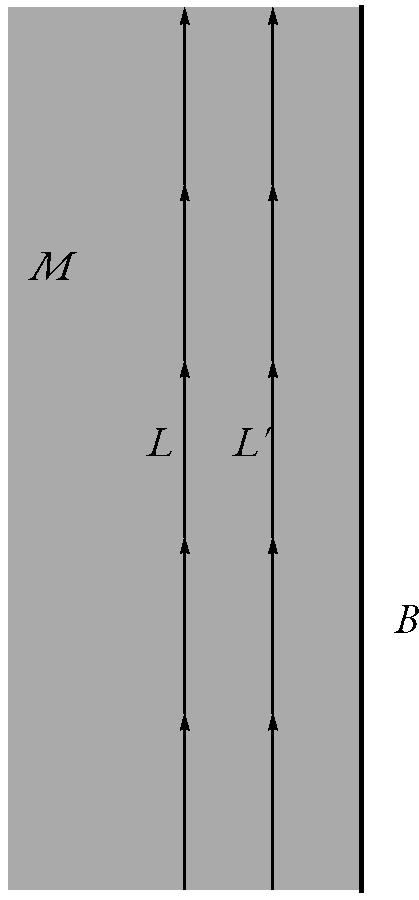
\includegraphics[scale=0.5]{figures/Wilson}
		\caption{The insertion of two Wilson lines approaching a boundary. They act associatively on the category of boundary conditions, and have actions commuting with one another.}
		\label{fig:wilson}
	\end{figure}
	
	 This functor will depend on the point $p \in C$ corresponding to the Wilson line. Consider the product $\mathcal M_{flat} (G, C) \times C$. There is a universal $G$-bundle $\mathcal E$ over this space, given by taking a point in $\mathcal M_{flat}$ and restricting the corresponding bundle to a point in $C$. 
	
	Given any coherent sheaf on $\mathcal M_{flat}$, we can tensor this with $R(\mathcal E)$. This is the action of the Wilson loop insertion on the space.
	
	Consider the structure sheaf $\mathcal O_x$ of a point $x \in \mathcal M_{flat}(\check G, C)$. For any representation $\check R$, the Wilson loop maps $\mathcal O_x$ to $\mathcal O_x \otimes \check{R}$.
	Thus $\mathcal O_x$ is an eigen-object for the functor $W_{\check R}(p)$, which acts on it by tensoring it with the vector space $\check R(\mathcal E_p)_x$. In fact, letting $p$ vary we see that it is an eigen-object for all $W_{\check R}(p)$. Another way of saying this is that the eigenvalue is the flat $\check G$-bundle $\check R(\mathcal E)_x$ on $C$.
	
	More directly, this flat bundle is obtained by taking the flat principle bundle on $C$ corresponding to $x$ and forming the associated bundle via $\check R$.
	
	The action of the `t Hooft operators is more difficult to see. They will end up acting by Hecke transformations on the space of boundary conditions. By Monotonen-Olive duality, it turns out that the brane corresponding to a fiber of the Hitchin fibration in $\mathcal M_H(G, C)$ is a common eigenobject for all operators.
	

\include{Chapters/Appendix}


% \include{ch-pastwork/chapter-pastwork}
% \include{ch-usage/chapter-usage}
% \include{ch-conclusion/chapter-conclusion}
% \appendix % all chapters following will be labeled as appendices
% \include{ch-appendicies/implementation}
% \include{ch-appendicies/printing}


% Make the bibliography single spaced
\singlespacing
\bibliographystyle{myunsrt}

% add the Bibliography to the Table of Contents
\cleardoublepage
\ifdefined\phantomsection
  \phantomsection  % makes hyperref recognize this section properly for pdf link
\else
\fi
\addcontentsline{toc}{chapter}{Bibliography}

% include your .bib file
\bibliography{thesis}

\end{document}

